%%%%%%%%%%%%%%%%%%%%%%%%%%%%%% Beamer-Presentation 2020 by C.Has%%%%%%%%%%%%%%%%%%%%%%
\documentclass[12pt, aspectratio=169]{beamer}
\usepackage{hyperref}
%%%%%%%%%%%%%%%%%%%%%%%%%%%%%%%%%%%%%%%%%%%%%%%%%%%%%%%%%%%%%%%%%%%%%%%%%%%%%%%%%%%%%%

%==================================== Preamble ==========================================
%-------------------------------- preamble.tex ------------------------------------------
\graphicspath{{gfx/}{setting/}}

%=================================== Packages ==============================================
\usepackage{ragged2e}\justifying
\usepackage{txfonts}
\usepackage{graphicx}
\usepackage{color}
\usepackage{booktabs}
\usepackage[numbers]{natbib}
\usepackage{bibentry}
\usepackage{appendixnumberbeamer}
\usepackage{pifont}
\usepackage{fontawesome}
\usepackage{textpos}
\usepackage{tabularray}
\usepackage{longtable}
\usepackage{makecell}
\usepackage{multirow}
\usepackage{graphicx}
\usepackage{calc} % used in third example
\usepackage{booktabs}
\usepackage{comment}
\usepackage{hyperref}
\UseTblrLibrary{booktabs}
\def\enroll{MGCUB}
%=================================== Themes ==============================================
%\usetheme{EastLansing}
\usetheme[secheader]{Madrid}

\useinnertheme{rectangles} 
%\useoutertheme{sidebar}
%\usecolortheme{wolverine}

\definecolor{myblue}{RGB}{51 51 178}
\definecolor{Gold}{rgb}{255 215 0}
%\usecolortheme[named=burgundy]{structure}

\usefonttheme{serif}
 
%========================= Beamer color/font/template ==================================== 
\setbeamersize{text margin left=7mm, text margin right=7mm} 
\setbeamertemplate{frametitle}[default][left, leftskip=2mm]
\setbeamertemplate{frametitle continuation}{\frametitle{References}}
\setbeamertemplate{bibliography item}[text] 
%\setbeamertemplate{page number in head/foot}[appendixframenumber]

\setbeamerfont{frametitle}{size=\large}
\setbeamerfont{title}{series=\bfseries, size=\Large}
\setbeamerfont{author}{series=\bfseries}
\setbeamerfont{institute}{series=\bfseries, size=\small}
\setbeamerfont{date}{series=\bfseries}
\setbeamerfont{frametitle}{series=\bfseries}
\setbeamerfont{itemize/enumerate body}{size=\footnotesize}
\setbeamerfont{itemize/enumerate subbody}{size=\scriptsize}
\setbeamerfont{itemize/enumerate subsubbody}{size=\scriptsize}


\setbeamercolor{link}{fg=black}
\setbeamercolor{frametitle}{bg=white, fg=black}
\setbeamercolor{title}{bg=white, fg=black}
\setbeamercolor{title}{bg=white, fg=black}
\setbeamercolor{author}{fg=white!5!black}
\setbeamercolor{institute}{fg=black}
\setbeamercolor{author in head/foot}{bg=gray!20!white, fg=black}
\setbeamercolor{title in head/foot}{bg=blue!30!white, fg=black}
\setbeamercolor{date in head/foot}{bg=white ,fg=black}
\setbeamercolor{page number in head/foot}{bg=blue!15!white, fg=black}
\setbeamercolor{section in head/foot}{bg=Gold!80!black ,fg=white }
%\setbeamercolor{palette quaternary}{bg=blue!10}

\setbeamertemplate{footline}{
\leavevmode\bfseries 	
\begin{beamercolorbox}[wd=0.20\paperwidth, ht=7pt, dp=2.5pt, center]{author in head/foot}
%\insertshortauthor~(\insertshortinstitute) %-----for and university--------(subham kumar (mgcub))
\Enroll %------enrollment number----------------------
\end{beamercolorbox}%
\begin{beamercolorbox}[wd=0.62\paperwidth, ht=7pt, dp=2.5pt, center]{title in head/foot}
\insertshorttitle
\end{beamercolorbox}%
\begin{beamercolorbox}[wd=0.12\paperwidth, ht=7pt, dp=2.5pt, center]{date in head/foot}
\insertshortdate
\end{beamercolorbox}%
\begin{beamercolorbox}[wd=0.06\paperwidth, ht=7pt, dp=2.5pt, center]{page number in head/foot}
\insertframenumber/\inserttotalframenumber
\end{beamercolorbox}%
}

\setbeamertemplate{headline}{
	\leavevmode\bfseries 	
	\begin{beamercolorbox}[wd=0.2\paperwidth, ht=7pt, dp=2.5pt, center]{section in head/foot}
	\insertsectionhead 
	\end{beamercolorbox}%
	\begin{beamercolorbox}[wd=0.8\paperwidth, ht=7pt, dp=2.5pt, center]{palette quaternary}
	\insertsectionnavigationhorizontal{0.8\paperwidth}{\hfill}{\hfill}
	\end{beamercolorbox}%
}


\setbeamertemplate{frametitle}{	
	\nointerlineskip		
	\begin{beamercolorbox}[wd=\paperwidth]{frametitle}
		\vskip-5pt \hskip3mm 
	\strut	\insertframetitle
		 \vskip5pt
	\end{beamercolorbox}%   
}

\setbeamertemplate{navigation symbols}{}
\setbeamertemplate{enumerate item}{\bfseries(\arabic{enumi})}
\setbeamertemplate{enumerate subitem}{\bfseries(\alph{enumii})}

%\setbeamertemplate{itemize item}{$\boldsymbol{\checkmark}$}
\setbeamertemplate{itemize item}{\bfseries\ding{113}}

\addtobeamertemplate{frametitle}{}{
\begin{textblock*}{1mm}(0.99\linewidth, -8mm)

\includegraphics[height=8.82mm, width=7.7mm]{setting/logo}
	\end{textblock*}
}

\setbeamertemplate{background canvas}{

\includegraphics[width=\paperwidth, height=\paperheight]{body_bg2}
}

%=================================== Others ==============================================
\setlength{\parskip}{5pt}

\let\oldbib\bibentry
\renewcommand{\bibentry}[1]{{\color{myblue}\bfseries\tiny[\oldbib{#1}]}}

%==========================================================================================
\setbeamertemplate{title page}[default]
%=============================== Title information ======================================
\title[Multi-view Stacked CNN-BiLSTM for Urban \boldmath{$PM_{2.5}$} Concentration Prediction of India’s Polluted Cities]{Multi-view Stacked CNN-BiLSTM (MvS CNN-BiLSTM) for Urban \boldmath{$PM_{2.5}$} Concentration Prediction of India’s Polluted Cities}
%\title[\boldmath{$PM_{2.5}$} Forecasting By Deep Learning Techniques]{Forecasting \boldmath{$PM_{2.5}$} of Some Indian Cites Using Deep Learning Techniques}
\subtitle{\scriptsize \textit{A dissertation-II submitted to the Mahatma Gandhi Central University
in partially fulfillment \\of the requirements
for the award of the degree of}\\
MASTER OF TECHONOLGY\\
\textit{IN}\\
COMPUTER SCIENCE \& ENGINEERING}
\def\Enroll{MGCU2021CSIT4029}  %------enrollment number Enter----------------------
\author[SUBHAM KUMAR]{\begin{tabular}{ccc} \begin{tabular}[c]{ccc} \footnotesize Presented By-\\ \small SUBHAM KUMAR\\ \scriptsize (\Enroll) \end{tabular} & \begin{tabular}[c]{ccc}
\includegraphics[scale=0.16]{setting/logo} \end{tabular} & \begin{tabular}[c]{ccc} \footnotesize Under the Supervision of\\ \small Dr. VIPIN KUMAR \\ \scriptsize Dept. CS\&IT, MGCU. \end{tabular} \end{tabular}}
%\author[Chandra Has]{Chandra Has\\ \tiny  chandrahashbti@gmail.com}
%\au[MGCUB]{VIP \\ VV}
\institute[MGCUB]{Department Of Computer Science And Information Technology \\ MAHATMA GANDHI CENTRAL UNIVERSITY, MOTIHARI \\ BIHAR - 845401, INDIA}

\date[\today]{\scriptsize \today}

%\titlegraphic{
\includegraphics[scale=0.08]{logo}}
%\logo{
\includegraphics[scale=0.08]{logo}}

%=================================== Main body========================================
\begin{document}

%% References	
%\bibliographystyle{apalike}
%\nobibliography{mybib}

%% Title frame
{
\setbeamertemplate{background canvas}{
	
\includegraphics[width=\paperwidth, height=\paperheight]{white_bg}
}	
\begin{frame}[plain, noframenumbering]
\maketitle
\end{frame}	
}
%--------------------------------------------------------------------------
\section[Outline]{}
%-------------------------------------------------------------------------

%% TOC
\begin{frame}{Outline}
	\tableofcontents	
\end{frame}
\begin{frame}{Publication}
	\begin{block}{}
		\textbf{1. Multi-view Stacked CNN-BiLSTM (MvS CNN-BiLSTM) for Urban $PM_{2.5}$ Concentration Prediction of India's Polluted Cities }\\
 		\footnotesize{Journal of Cleaner Protecation, Elsevier  \textbf{(Impact Factor: 11.1)}  Indexed by \textbf{SCI}\\ (Submitted on $14^{th}$ Aug 2023)\\
		Authors- \textbf{Subham Kumar and  Vipin Kumar}}
	\end{block}
\end{frame}
%------------------------------------------------------------------------
\section{Introduction}
%-------------------------------------------------------------------------
\begin{frame}{Introduction}
	\begin{columns}
		\column[]{0.5\textwidth}
		\begin{itemize}
			\item   Air pollution may harm human health in a variety of ways, including respiratory difficulties, cardiovascular illness, and cancer. Air pollution is also harmful to the environment.
			\item According to the IQAir 2021 report, 36 Indian cities are among the top 50 most polluted cities in the world. \footnote[1]{\href{https://www.iqair.com/world-most-polluted-cities/world-air-quality-report-2021-en.pdf}{https://www.iqair.com/world-most-polluted-cities/world-air-quality-report-2021-en.pdf}} \\
			\item The most effective factor in AQI is $PM_{2.5}$.
		\end{itemize}
		\column[]{0.5\textwidth}
		\begin{figure}
			\centering
			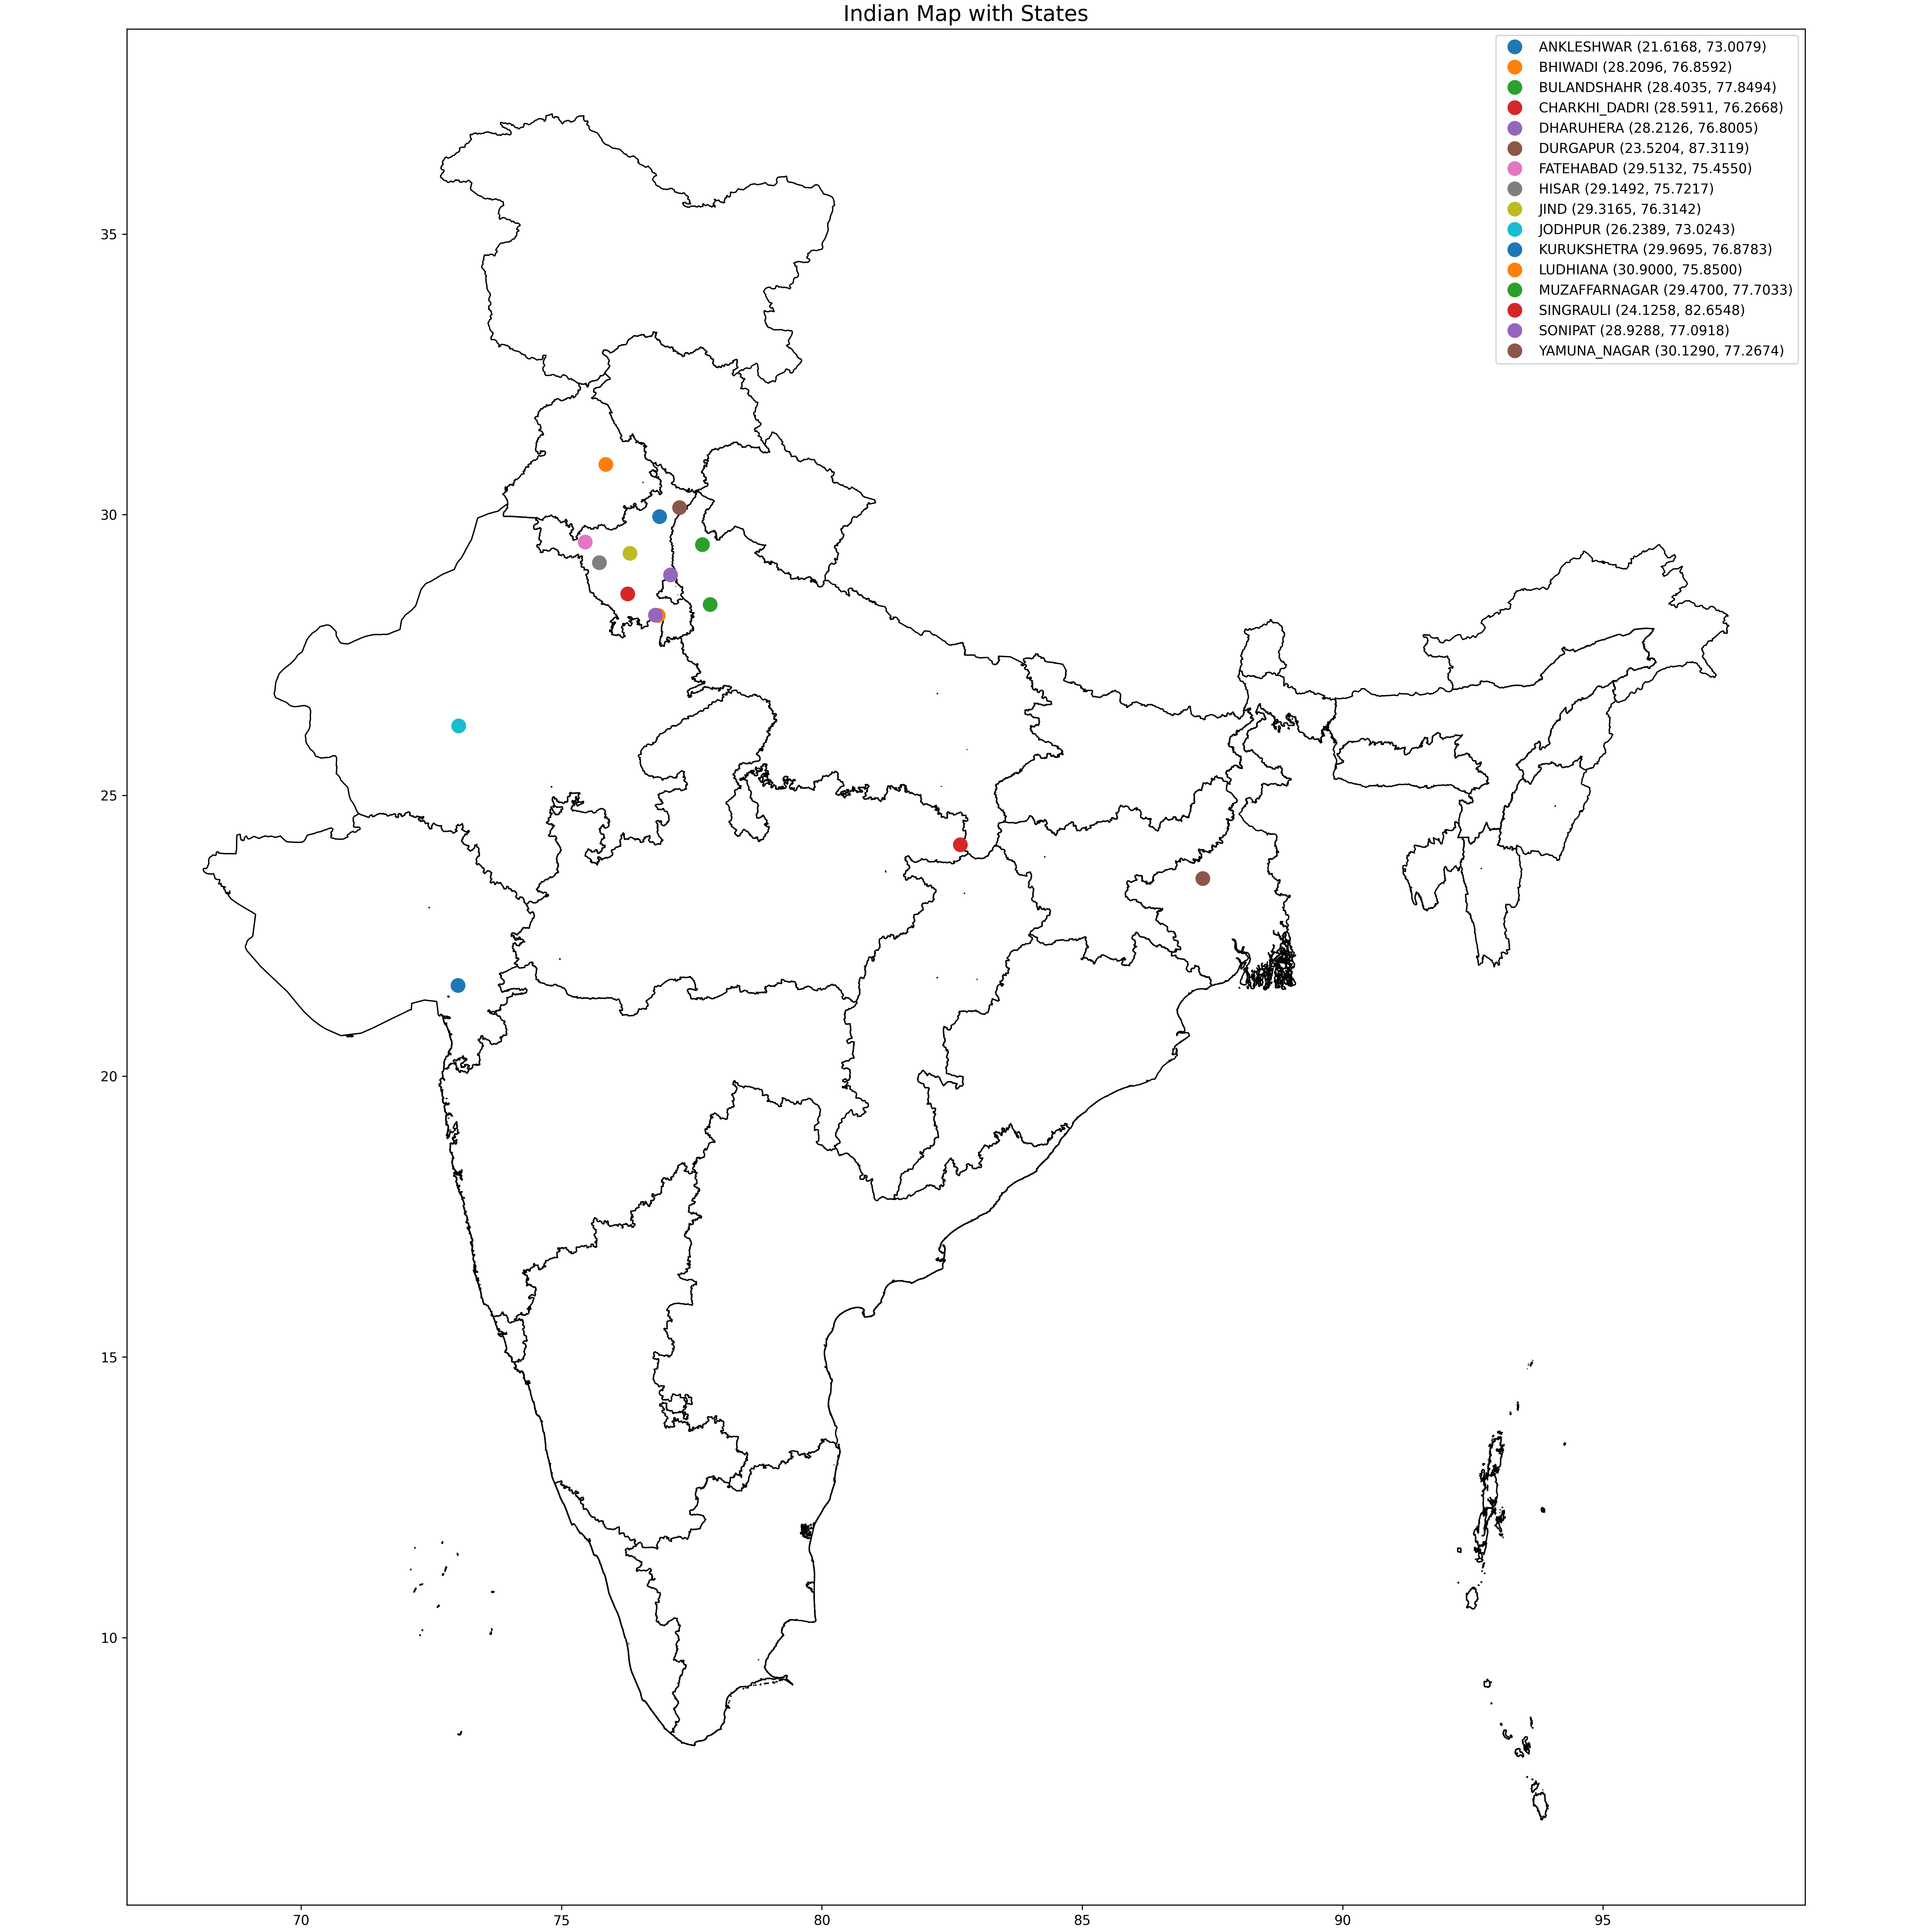
\includegraphics[scale=.12]{India_Map}\\ 
			\scriptsize{Figure 1: Geographical reactivation where data pick from.}
		\end{figure}
	\end{columns}
	
\end{frame}




 
%--------------------------------------------------------------------------
\section[Literature]{Literature Review}%, Blocks, and Columns
%--------------------------------------------------------------------------
\begin{frame}{Literature Review}
	\centering
	\scriptsize {TABLE 2.1: summary of recent state-of-art based on Data,  Model proposed,  Performance measures and Research gap.}\\
	\begin{table}
		\centering
		\begin{tabular}{|p{0.03\linewidth}|p{0.3\linewidth}|p{0.14\linewidth}|p{0.16\linewidth}|p{0.21\linewidth}|}
			\hline
			\footnotesize \textbf {Ref.} & \footnotesize \textbf { Data} & \footnotesize \textbf {Performance Measures } & \footnotesize \textbf {Model} & \footnotesize \textbf {Research Gap }  \\ \hline
			\scriptsize \cite{li2023nested}                \scriptsize & North America (Jan 21 -Sep 21)   Hourly Data collected from US EPA                                       \scriptsize & MAE:  2.81                                                                                               \scriptsize & GNN-LSTM Fully Connected (FC) network                              \scriptsize & Adding more variables and new data preprocessing technique for enhancing model.                                    \\ \hline
			\scriptsize \cite{pruthi2022low}           \scriptsize & Delhi  India (18 -21) Daily Data collected from   CPCB India.                                            \scriptsize & Correlation coefficients:  {[}0.96, 0.98{]} (1   day),  {[}0.86, 0.93{]} (2 days) \scriptsize & Wavelet,  ANFIS,  PSO                                                 \scriptsize &  Adding more historical data for enhance model.                                                  \\ \hline
			\scriptsize \cite{menares2021forecasting}             \scriptsize & Santiago Chile (05 - 19) Hourly   Data provided by Ministry of the Environment                           \scriptsize & RMSE 3.88,  MAE 2.52,  $R^2$ 0.94                                                                            \scriptsize & LSTM Deep Feedforward Neural Network                               \scriptsize & Add more pollutants for enhance the model.               \\ \hline
			\scriptsize \cite{zhu2023investigation}            \scriptsize & Shanghai china (2014-05-13 to 2020-12-31)   Hourly Data from Ministry of Environmental Protection \scriptsize & RMSE 3.88,  MAE 2.52,  $R^2$ 0.94                                                                            \scriptsize & Parallel multi-input 1D-CNN-biLSTM   model                          \scriptsize & add  factory data ,  creating a Smartphone Application for PM2.5 forecasting.                                                         \\ \hline
	 \end{tabular}
	\end{table}
\end{frame}

\begin{frame}{Literature Review  \tiny{Continue...}}
	\centering
	\scriptsize {TABLE 2.1: continuation of summary of recent state-of-art based on Data,  Model proposed,  Performance measures and Research gap.}\\
	\begin{table}
		\centering
		\begin{tabular}{|p{0.03\linewidth}|p{0.29\linewidth}|p{0.15\linewidth}|p{0.16\linewidth}|p{0.21\linewidth}|}
			\hline
			\footnotesize \textbf {Ref.} & \footnotesize \textbf { Data} & \footnotesize \textbf {Performance Measures } & \footnotesize \textbf {Model} & \footnotesize \textbf {Research Gap }  \\ \hline
			\scriptsize \cite{MANDAL2023137036} \scriptsize & Delhi India (1 Jan 2018- 30 Nov 2019) 15 min interval data collected from CPCB Inda. \scriptsize &$R^2=0.75$,  $RMSE=25.13$,  $MAE: 21.28$ \scriptsize & Cluster-based Graph Neural Network (SA-GNN) \scriptsize & Add activation function, add more historical data \\ \hline
			\scriptsize \cite{MA2019117729} \scriptsize & Washington, US (1st January to 31st January 2017) hourly data collected from US (EPA) \scriptsize & $RMSE = 0.043$ \scriptsize & Geo-LSTM \scriptsize & Add more Data with more futures of Data.  \\ \hline
			\scriptsize \cite{ZHANG2022134890}\scriptsize & Sichuan Basin (January 1,  2019,  to December 31,  2019) Hourly data collected from  China Environmental Monitoring Center  \scriptsize & $R^2= 0.917$, $RMSE=7.4$ \scriptsize & data-driven spatial autocorrelation terms (DDW-RF) \scriptsize & necessary to select more appropriate high-resolution variables. \\ \hline
			\scriptsize \cite{TIAN2022134048} \scriptsize & Beijing,  Tianjin,  Dalian,  and Yantai (1600 hour) China \scriptsize & $MAPE=6.0819$, $RMSE=11.8654$, $R^2=0.9754$ \scriptsize &  multi-objective optimisation algorithm \scriptsize & Add more pollutants, improving accuracy \\ \hline
	\end{tabular}
	\end{table}
\end{frame}

\begin{frame}{Literature Review  \tiny{Continue...}}
	\centering
	\scriptsize {TABLE 2.1: continuation of summary of recent state-of-art based on Data,  Model proposed,  Performance measures and Research gap.}\\
	\begin{table}
		\centering
		\begin{tabular}{|p{0.03\linewidth}|p{0.29\linewidth}|p{0.15\linewidth}|p{0.16\linewidth}|p{0.21\linewidth}|}
			\hline
			\footnotesize \textbf {Ref.} & \footnotesize \textbf { Data} & \footnotesize \textbf {Performance Measures } & \footnotesize \textbf {Model} & \footnotesize \textbf {Research Gap }  \\ \hline
			\scriptsize \cite{DAI2022131898} \scriptsize &shaanxi province ( January 1,  2016, to December 31,  2020 ) daily data \scriptsize & $RMSE=0.3997$, $MAPE=0.14599$, $MAE=0.2871$ \scriptsize &GBoost-MLP based on GARCH model \scriptsize & apply deep learning model \\  \hline
 			\scriptsize \cite{AGGARWAL2021129660} \scriptsize & India (January 2016 to December 2018) 15-minute interval  \scriptsize & $RMSE=19.89, 25.88$ ,  $R^2=0.96, 0.9$ \scriptsize &lstm\scriptsize &apply more pollutants \\\hline
			 \scriptsize \cite{kim2022short}         \scriptsize & Seoul South Korea ( July 2018 to   June 2021) Deliy Data                                                 \scriptsize & bias = -0.25\% to -0.10\%,  RMSE =   32.45\%-33.23\%,  $R^2$ = 0.83-0.86                                     \scriptsize & LGB algorithm                                                       \scriptsize & Add more data for enhance the model.                                                                            \\ \hline
			 \scriptsize \cite{lee2021potential}            \scriptsize & Seoul Korea (16 -19) Hourly Data collected from ground-based observation stations                      \scriptsize & $R^2$ values:  0.61 and 0.78                                                                                \scriptsize & GOCI-based model, MAIAC-based model                                \scriptsize & Add more pollutants and Data for enhance the model.                                                                   \\ \hline
		\end{tabular}
	\end{table}
\end{frame}

\begin{frame}{Literature Review  \tiny{Continue...}}
	\centering
	\scriptsize {TABLE 2.1: continuation of summary of recent state-of-art based on Data,  Model proposed,  Performance measures and Research gap.}\\
	\begin{table}
		\centering
		\begin{tabular}{|p{0.03\linewidth}|p{0.29\linewidth}|p{0.15\linewidth}|p{0.16\linewidth}|p{0.21\linewidth}|}
			\hline
			\footnotesize \textbf {Ref.} & \footnotesize \textbf { Data} & \footnotesize \textbf {Performance Measures } & \footnotesize \textbf {Model} & \footnotesize \textbf {Research Gap }  \\ \hline
			\scriptsize \cite{samal2021multi}  \scriptsize & Talcher India (02/02/2018 to   04/07/2020) per 15 min Data collected from CPCB india.                    \scriptsize & RMSE values:  93\%  and 90\% better than GRU                                                              \scriptsize & MTCAN model                                                         \scriptsize & add meteorological factors and traffic data for the enhanced model.                                                               \\\hline
			\scriptsize \cite{kurnaz2022prediction}          \scriptsize & Sakarya Urbanization (   01.08.2018 and 31.07.2020) Daliy Data provided from e Ministry of Environment   \scriptsize & RMSE:  2.84–14.09                                                                                       \scriptsize & RNN                                                                 \scriptsize & Add more pollutants and Data for enhance model.    \\\hline
			\scriptsize \cite{das2022prediction}           \scriptsize & Istanbul Basaksehir (01.01.2021   and 09.02.2022) Hourly data taken from Ministry of Environment         \scriptsize & RMSE: 10.229478                                                                                          \scriptsize & LSTM16                                                              \scriptsize & add more pollutants and  meteorological Data for enhance model. data.                                          \\\hline
			\scriptsize \cite{natsagdorj2023prediction}              \scriptsize & Ulaanbaatar Mongolia  (June 1,  2018, to  April 30,  2020) Hourly Data from U.S.   Embassy in Mongolia      \scriptsize & RMSE: 11.77                                                                                              \scriptsize & CNN-LSTM                                                            \scriptsize & Add more Data and atmospheric Data for enhance the model.  \\\hline
		 \end{tabular}
	\end{table}
\end{frame}

\begin{frame}{Literature Review  \tiny{Continue...}}
	\centering
	\scriptsize {TABLE 2.1: continuation of summary of recent state-of-art based on Data,  Model proposed,  Performance measures and Research gap.}\\
	\begin{table}
		\centering
		\begin{tabular}{|p{0.03\linewidth}|p{0.29\linewidth}|p{0.15\linewidth}|p{0.16\linewidth}|p{0.21\linewidth}|}
			\hline
			\footnotesize \textbf {Ref.} & \footnotesize \textbf { Data} & \footnotesize \textbf {Performance Measures } & \footnotesize \textbf {Model} & \footnotesize \textbf {Research Gap }  \\ \hline
			\scriptsize  \cite{eren2023predicting}         \scriptsize & Istanbul (15-19) Hourly Data collected from Kathane air quality monitoring station                     \scriptsize & $R^2$:  0.98                                                                                               \scriptsize & LSTM+LSTM                                                           \scriptsize & Add more pollutants and Data for enhance the model.           \\\hline
			\scriptsize \cite{zhu2023deep}           \scriptsize & Italian city ( March 2004 to   February 2005 ) Hourly Data collected from Kaggle \scriptsize & 91\% Prediction accuracy \scriptsize & Conv.LSTM                                                           \scriptsize & Deploy deep leading models for classification.  \\\hline
			\scriptsize \cite{ma2019improving}               \scriptsize & Guangdong China (3 years) Hourly   Data collected from Guangdong province.                               \scriptsize & RMSE: 8.652,  MAE: 6.184,    MAPE: 27.909                                                                   \scriptsize & TL-BLSTM                                                            \scriptsize & utilising transfer learning techniques and adding more data to enhance the model.     \\\hline
			\scriptsize \cite{qin2019novel}       \scriptsize & Shanghi (2015-2017) Daliy Data collected   manually  \scriptsize & RMSE:  14.3   \scriptsize & CNN+LSTM     \scriptsize &  Add more data for enhance model. \\\hline
			\end{tabular}
	\end{table}
\end{frame}

\begin{frame}{Literature Review  \tiny{Continue...}}
	\centering
	\scriptsize {TABLE 2.1: continuation of summary of recent state-of-art based on Data,  Model proposed,  Performance measures and Research gap.}\\
	\begin{table}
		\centering
		\begin{tabular}{|p{0.03\linewidth}|p{0.29\linewidth}|p{0.15\linewidth}|p{0.16\linewidth}|p{0.21\linewidth}|}
			\hline
			\footnotesize \textbf {Ref.} & \footnotesize \textbf { Data} & \footnotesize \textbf {Performance Measures } & \footnotesize \textbf {Model} & \footnotesize \textbf {Research Gap }  \\ \hline
			\scriptsize  \cite{li2017long}          \scriptsize & Beijing China (Jan 2014 -may   2016) Hourly Data collected from Ministry of environmental protection.    \scriptsize & RMSE: 12.6,  MAE: 5.46,  MAPE:  11.93                                                                        \scriptsize & LSTM NN extended(LSTME)                                             \scriptsize & Adding more pollutants to enhance the model.                                           \\\hline
			\scriptsize \cite{du2019deep}         \scriptsize & Beijing China (   01/01/2010-01/31/2010) Hourly Data collected from0 uci.                                 \scriptsize & RMSE: 77.38,  MAE: 54.58                                                                                   \scriptsize & Deep Air Quality Forecasting   Using Hybrid Deep Learning Framework \scriptsize & Add more Data for model enhancing.\\\hline
			\scriptsize \cite{nath2021long}       \scriptsize & Kolkata India (Jan 16 - Feb 20)  Daily Data collected from CPCB   India.                               \scriptsize & RMSE: 18.8,  MAE: 15.88                                                                                    \scriptsize & Autoencoder based LSTM                                             \scriptsize &  include exogenous variables for enhance the model. \\ \hline
		   \end{tabular}
	\end{table}
\end{frame}





%.............................................................................
\section[Problem \& Objectives]{Problem Definition \& Objectives of Research}
%.............................................................................
\begin{frame}{Problem Definition \& Objectives of Research}
	\begin{itemize}
		\item Problem Definition:
		\par Forecasting air pollution is critical in many aspects, including:
		\begin{itemize}
			\item Public health.\\
			\item Environmental management. \\
			\item Urban planning.\\
			\item Climate change.\\
		\end{itemize}
		\par Overall, forecasting air pollution levels is critical for public health, environmental preservation, and supporting sustainable development.

		\item Objectives of Research :
		\begin{itemize}
			\item Collect Real-Time Data
			\item To optimize models for increased forecasting accuracy. \\
			\item To create a novel model for $PM_{2.5}$ forecasting.\\
		\end{itemize}
	\end{itemize}
\end{frame}
  

%.............................................................................
\section[Methodology]{Methodology}
\subsection{Dataset Description}
%.............................................................................
\begin{frame}{Dataset Description}
	\begin{columns}
		\column[]{0.4\textwidth}
		\begin{itemize}
			\item \textbf{Data Source : }CPCB India \footnote{\href{https://app.cpcbccr.com/ccr/\#/caaqm-dashboard-all/caaqm-landing/data}{\footnotesize {www.app.cpcbccr.com/ccr/\#/caaqm-dashboard-all/caaqm-landing/data,\\ \textit{ Date of Access : 04-12-2022}}}}.
			\item \textbf{No. of Feature : }One ($PM_{2.5}$).
			\item \textbf{Data format : }CSV.
			\item \textbf{Data Type : }Time Series.
			\item Hourly Data
		\end{itemize}
		\column[]{0.6\textwidth}
		\begin{figure}
			\centering
			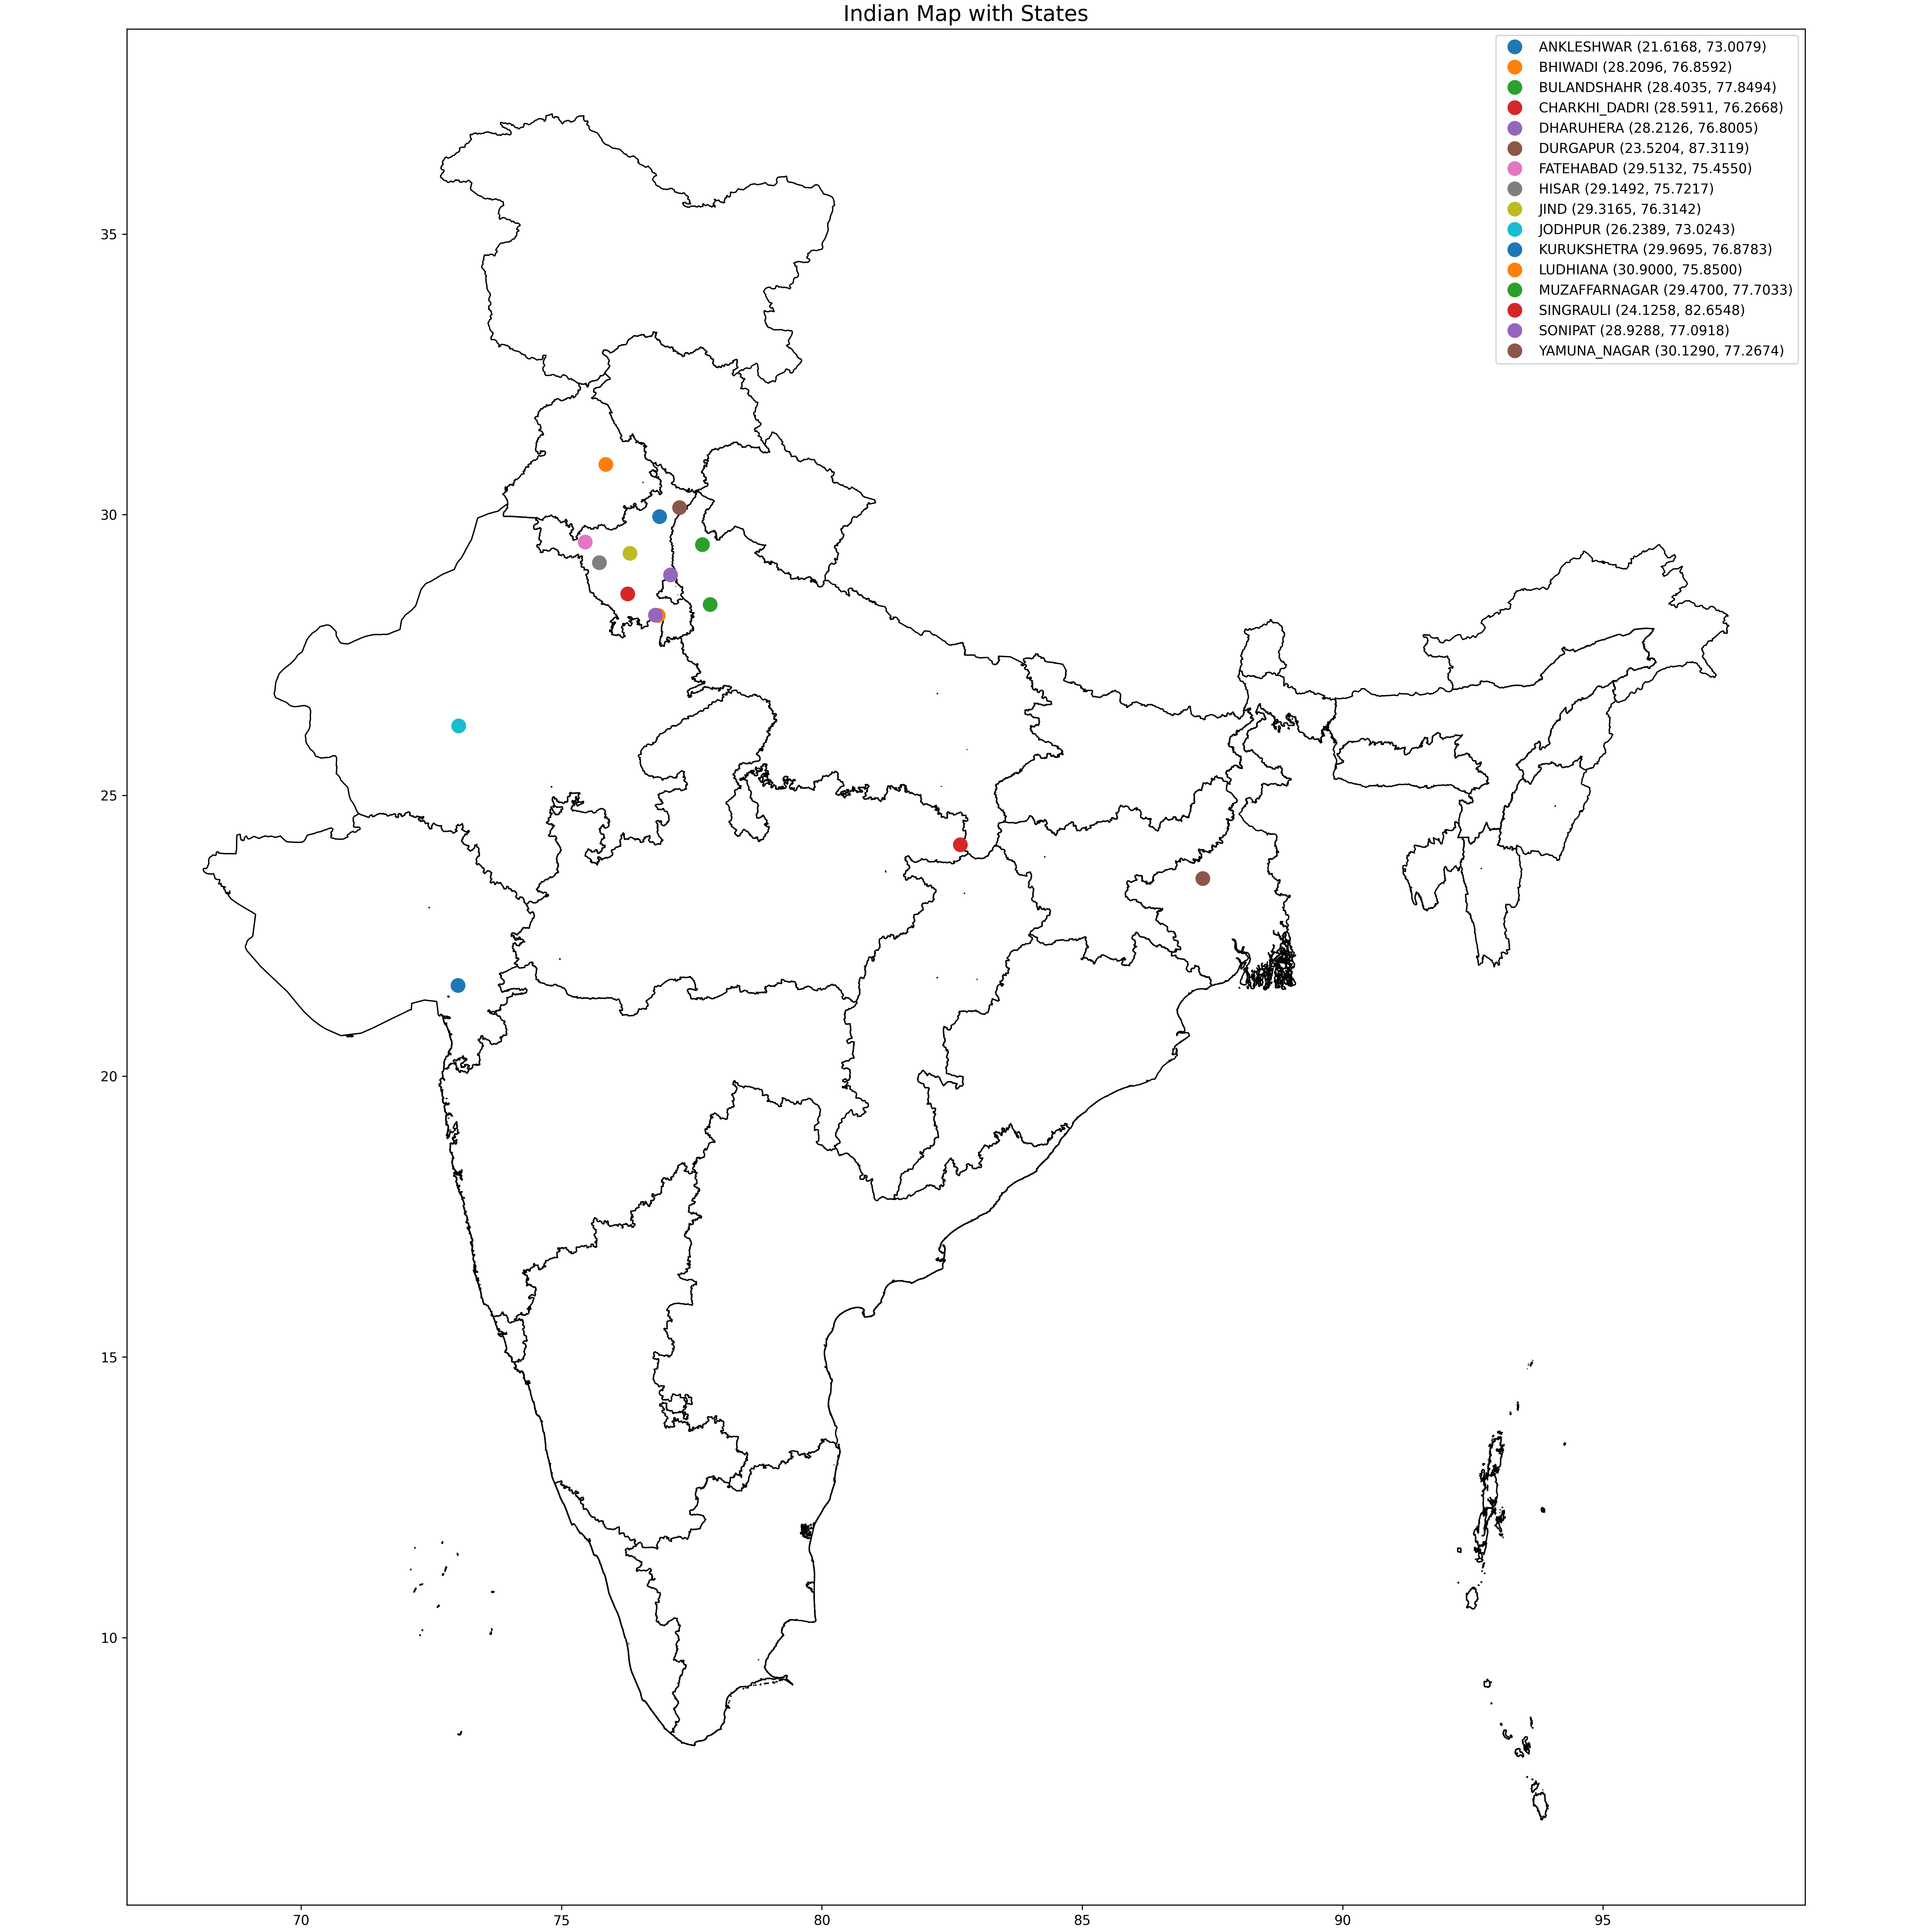
\includegraphics[scale=.12]{India_Map}\\ 
			\scriptsize{Figure 4.1: Geographical reactivation where data pick from.}
		\end{figure}
	\end{columns}
	
\end{frame}





\begin{frame}{Dataset Description  \tiny{Continue...}}
	\centering
	\scriptsize {TABLE 4.1: Statistical exploratory data analyses $($EDA$)$ of 17 Time Series Datasets of polluted Indian cities based on $PM_{2.5}$ \cite{bhawan2020central}.}\\
	\begin{table}
		\begin{tabular}{|p{0.17\linewidth}|p{0.09\linewidth}|p{0.05\linewidth}|p{0.05\linewidth}|p{0.05\linewidth}|p{0.04\linewidth}|p{0.05\linewidth}|p{0.05\linewidth}|p{0.06\linewidth}|p{0.07\linewidth}|} \hline
		\footnotesize \textbf{Cities}&\footnotesize \textbf{Year} & \footnotesize \textbf{Count} & \footnotesize \textbf{Mean} & \footnotesize \textbf{Std} & \footnotesize \textbf{Min} & \footnotesize \textbf{25\%} &\footnotesize \textbf{50\%} &\footnotesize \textbf{75\%} & \footnotesize \textbf{Max}  \\ \hline
		
		\textbf{BHIWADI}          & 2017-2022  & 43394   & 108.03 & 79.76  & 0.02 & 55.22   & 97.32       & 135.36 & 999.99 \\ \hline
		\textbf{JODHPUR}     & 2015-2022 &\textbf{61409} & 84.31 & 56.18 & 0.18 & 53.25   & 84.31 & 93.42   & 999.99 \\ \hline
		\textbf{SINGRAULI}    & 2017-2022 & 43695   & 84.08 & 78.33 & 0.25 & 32.25   & 66          & 111.25  & 985    \\ \hline
		\textbf{ANKLESHWAR}   & 2019-2022  & 33535     & 58.47 & 35.83 & 0.51 & 32.75   & 58.47 & 72.24   & 977.39 \\ \hline 
		\textbf{LUDHIANA}        & 2017-2022  & 49010  & 54.18 & 41.73 & 0.07 & 29.7    & 47.66       & 64.88   & 999.99 \\ \hline
		\textbf{DURGAPUR}       & 2020-2022 & \textbf{17434}   & 71.67 & 46.20 & 0.33 & 37.47 & 62.05      & 98.03 & 565.41 \\ \hline 
		\textbf{YAMUNA\_NAGAR}  & 2019-2022 & 34299   & 77.86  & 52.31 & 0.1  & 43.8    & 69.91       & 94.28   & 930    \\ \hline
		\textbf{CHARKHI\_DADRI}  & 2020-2022  & 24099   & 80.19 & 62.81 & 0.01 & 39.54  & 77.92       & 94.49  & 995.1  \\ \hline 
		\textbf{JIND  }           & 2019-2022 & 34145 & 81.21 & 71.20 & 0.2  & 38.99   & 61.45       & 98.25   & 845.6  \\ \hline 
		\textbf{KURUKSHETRA}    & 2019-2022  & 34208 & 68.75& 53.80 & 0.46 & 33.33   & 56.38       & 87.56   & 962.7  \\ \hline 
		\textbf{SONIPAT}        & 2019-2022  & 34362  & 54.88 & 43.21  & 0.02 & 27.87   & 49.4        & 62.72   & 543.1  \\ \hline 
		\textbf{DHARUHERA}     & 2019-2022 & 34265 & 78.86 & 59.21 & 0.02 & 40.9    & 70.32       & 92.85   & 838.9  \\ \hline
		\textbf{AMBALA}         & 2019-2022 & 34174 & 61.58 & 45.39 & 0.02 & 32.94   & 51.27       & 76.18 & 754.89 \\ \hline
		\textbf{HISAR}          & 2019-2022 & 34143 & 86.22 & 71.02 & 0.63 & 42.62   & 69.33       & 102.89 & 999.99 \\ \hline 
		\textbf{FATEHABAD}      & 2019-2022 & 34160 & 63.01 & 60.46 & 0.07 & 32.63   & 49.01       & 72.5    & 999.99 \\ \hline
		\textbf{BULANDSHAHR}  & 2018-2022 & 39869  & 90.53 & 85.08 & 0.25 & 34      & 63.75       & 120.25  & 985    \\ \hline 
		\textbf{MUZAFFARNAGAR}  & 2018-2022 & 38786 & 89.29 & 72.84  & 1    & 42.75   & 81.25       & 102.25  & 986    \\ \hline
		\end{tabular}
	\end{table}
\end{frame}


\begin{frame}{Dataset Description \tiny{Continue...}}
	\centering
	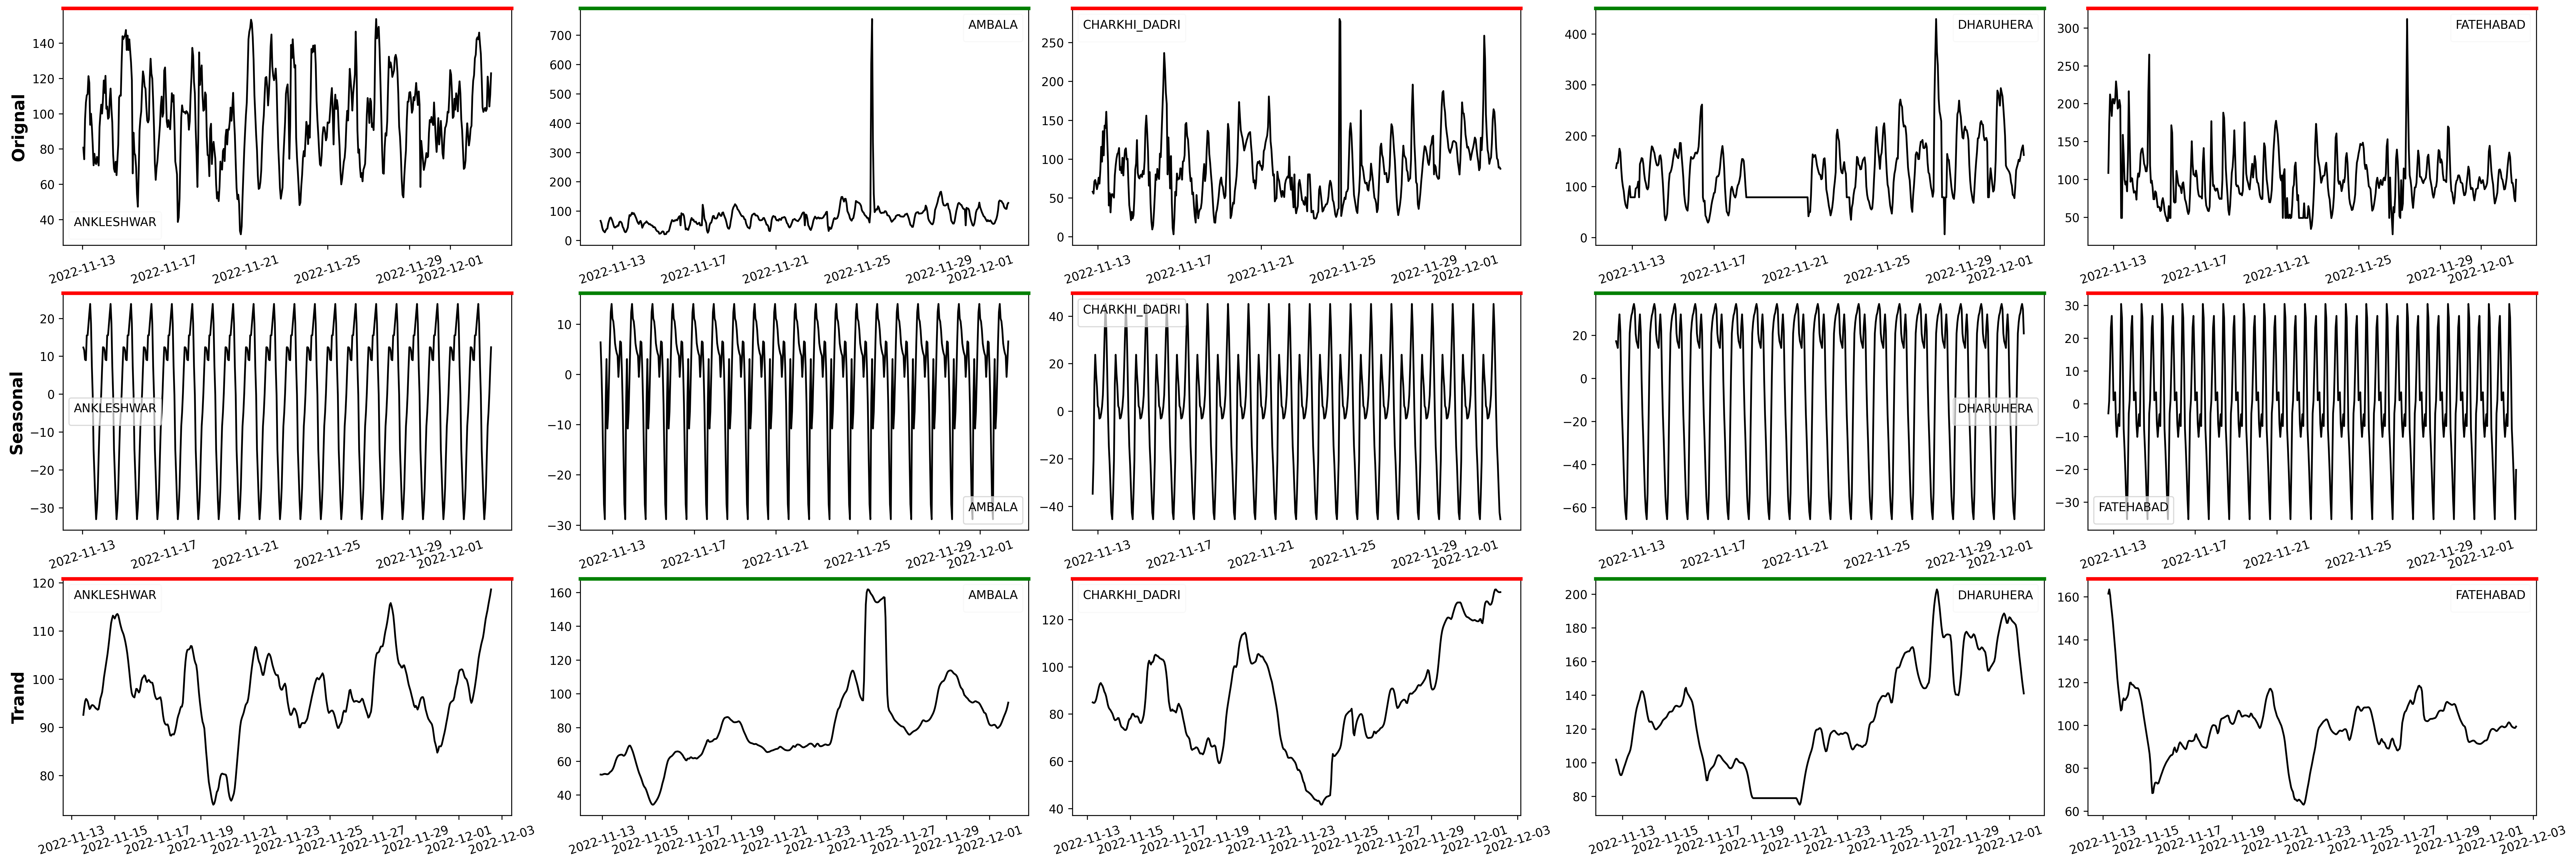
\includegraphics[scale=.19]{1}\\ 
	\scriptsize{FIGURE 4.2: Decomposition of 17 data sets based on trend, seasonal, and original dataset..}
\end{frame}

\begin{frame}{Dataset Description \tiny{Continue...}}
	\centering
	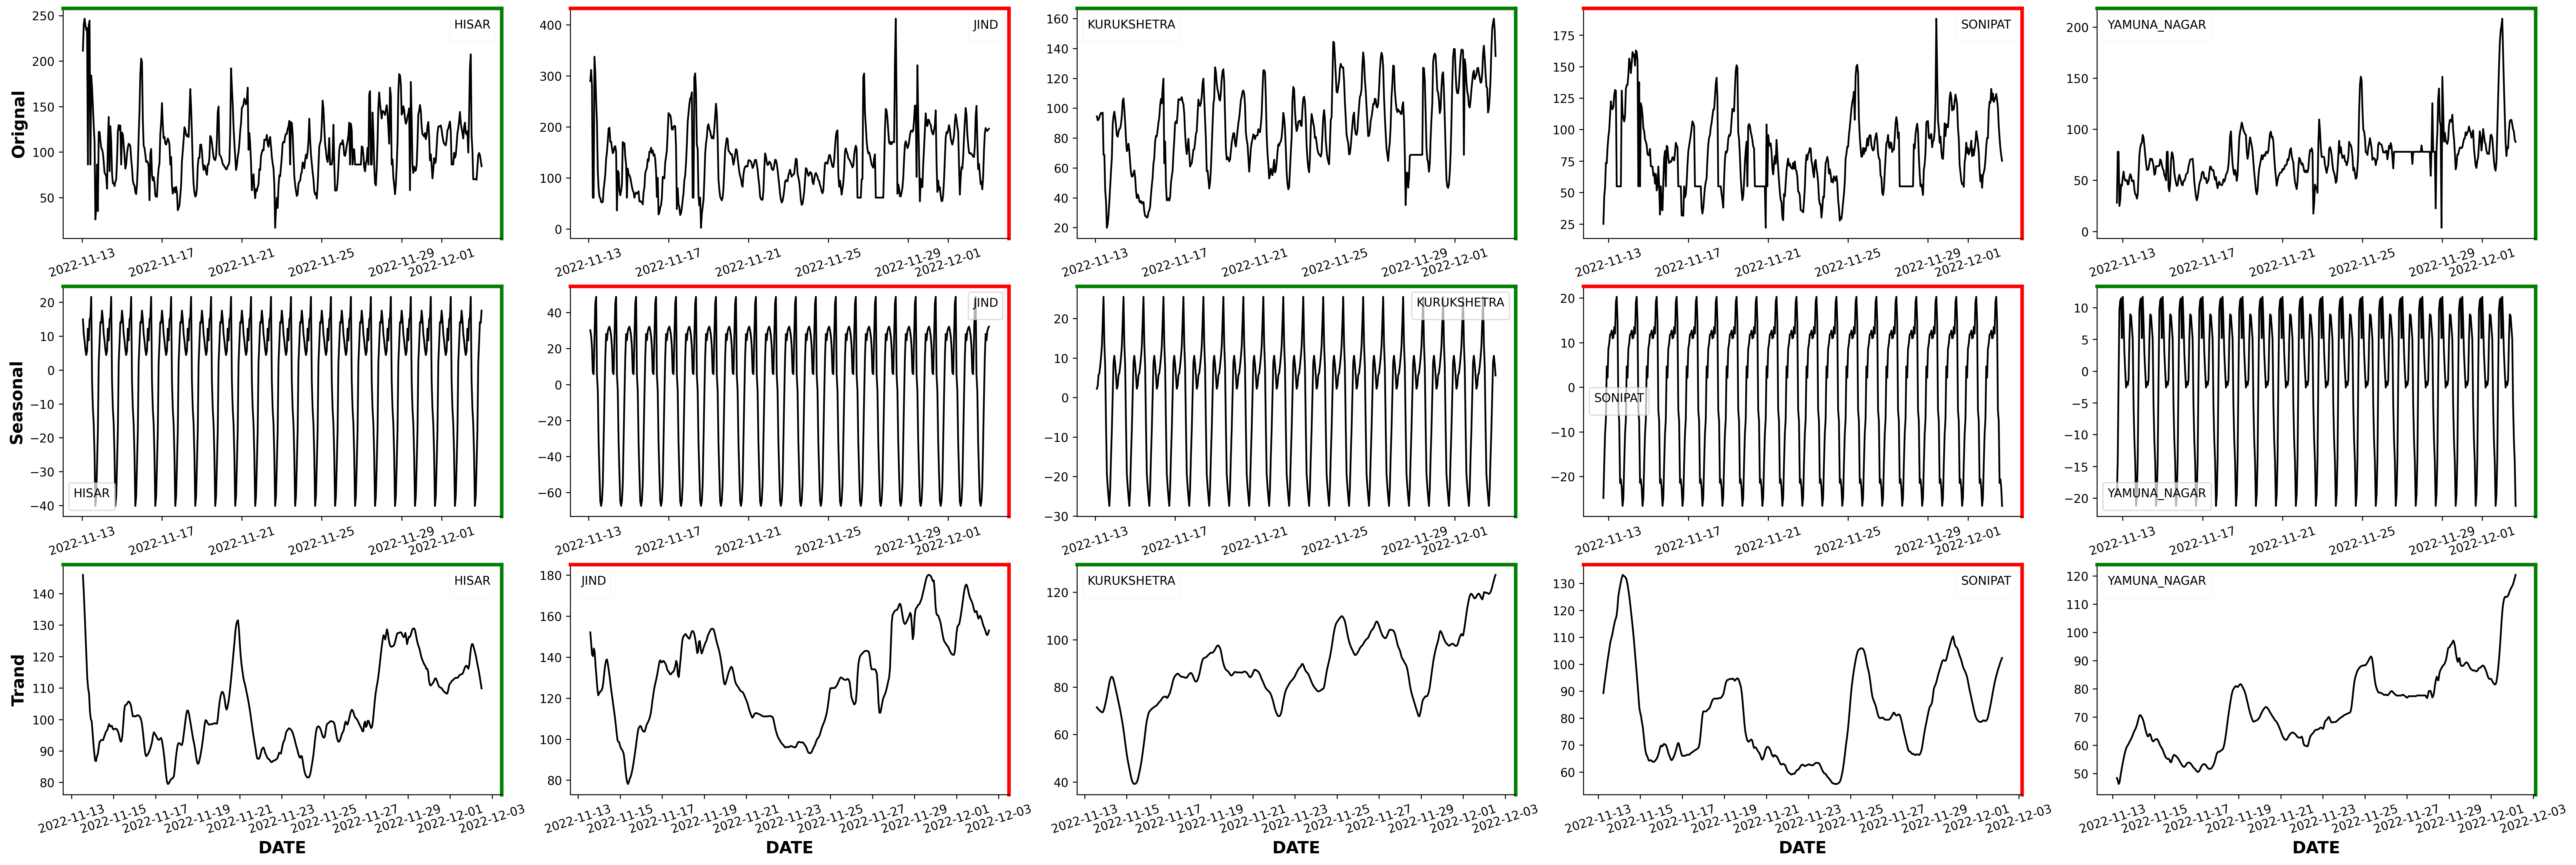
\includegraphics[scale=.19]{2}\\
	\scriptsize{FIGURE 4.3: Continuation of decomposition of 17 data sets based on trend, seasonal, and original dataset.}
\end{frame}

\begin{frame}{Dataset Description \tiny{Continue...}}
	\centering
	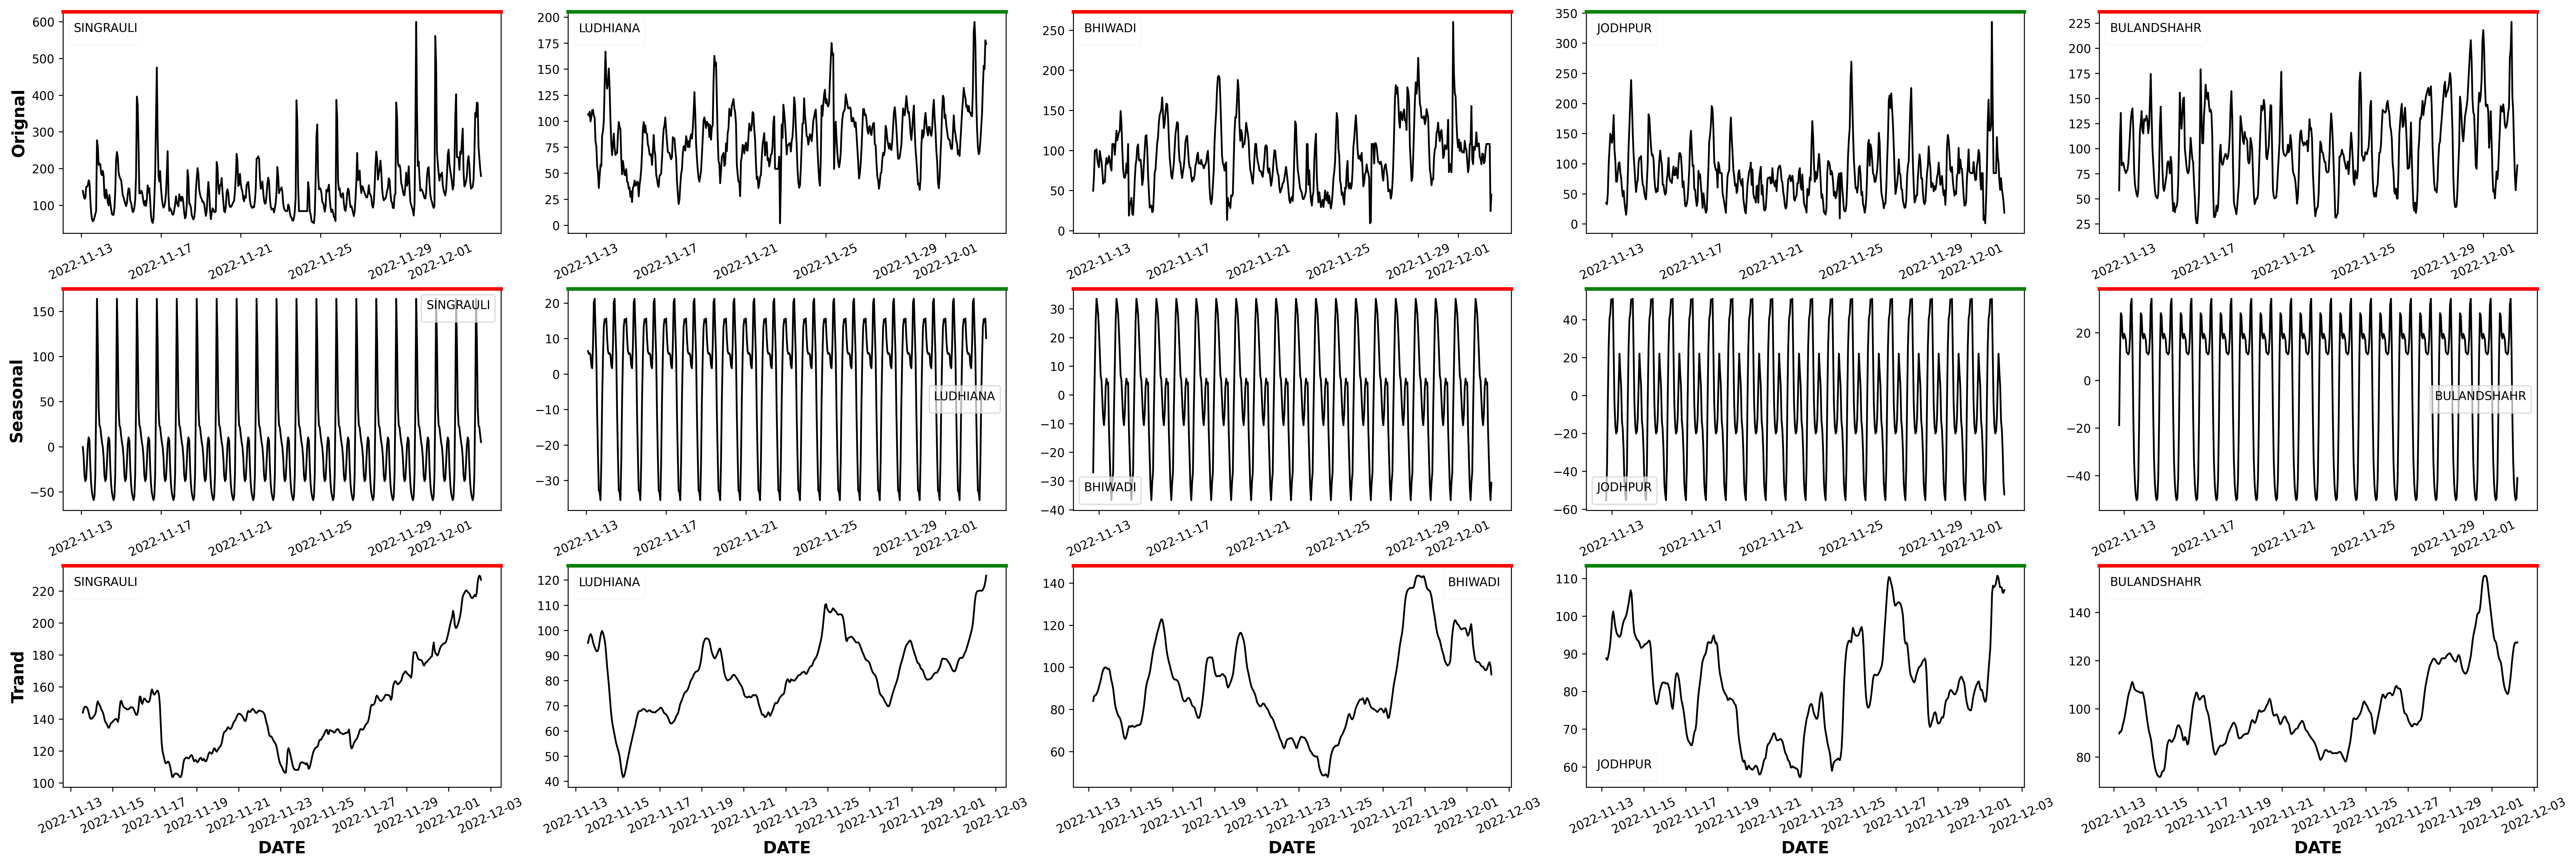
\includegraphics[scale=.19]{3}\\
	\scriptsize{FIGURE 4.4: Continuation of decomposition of 17 data sets based on trend, seasonal, and original dataset.}
\end{frame}

\begin{frame}{Dataset Description \tiny{Continue...}}
	\centering
	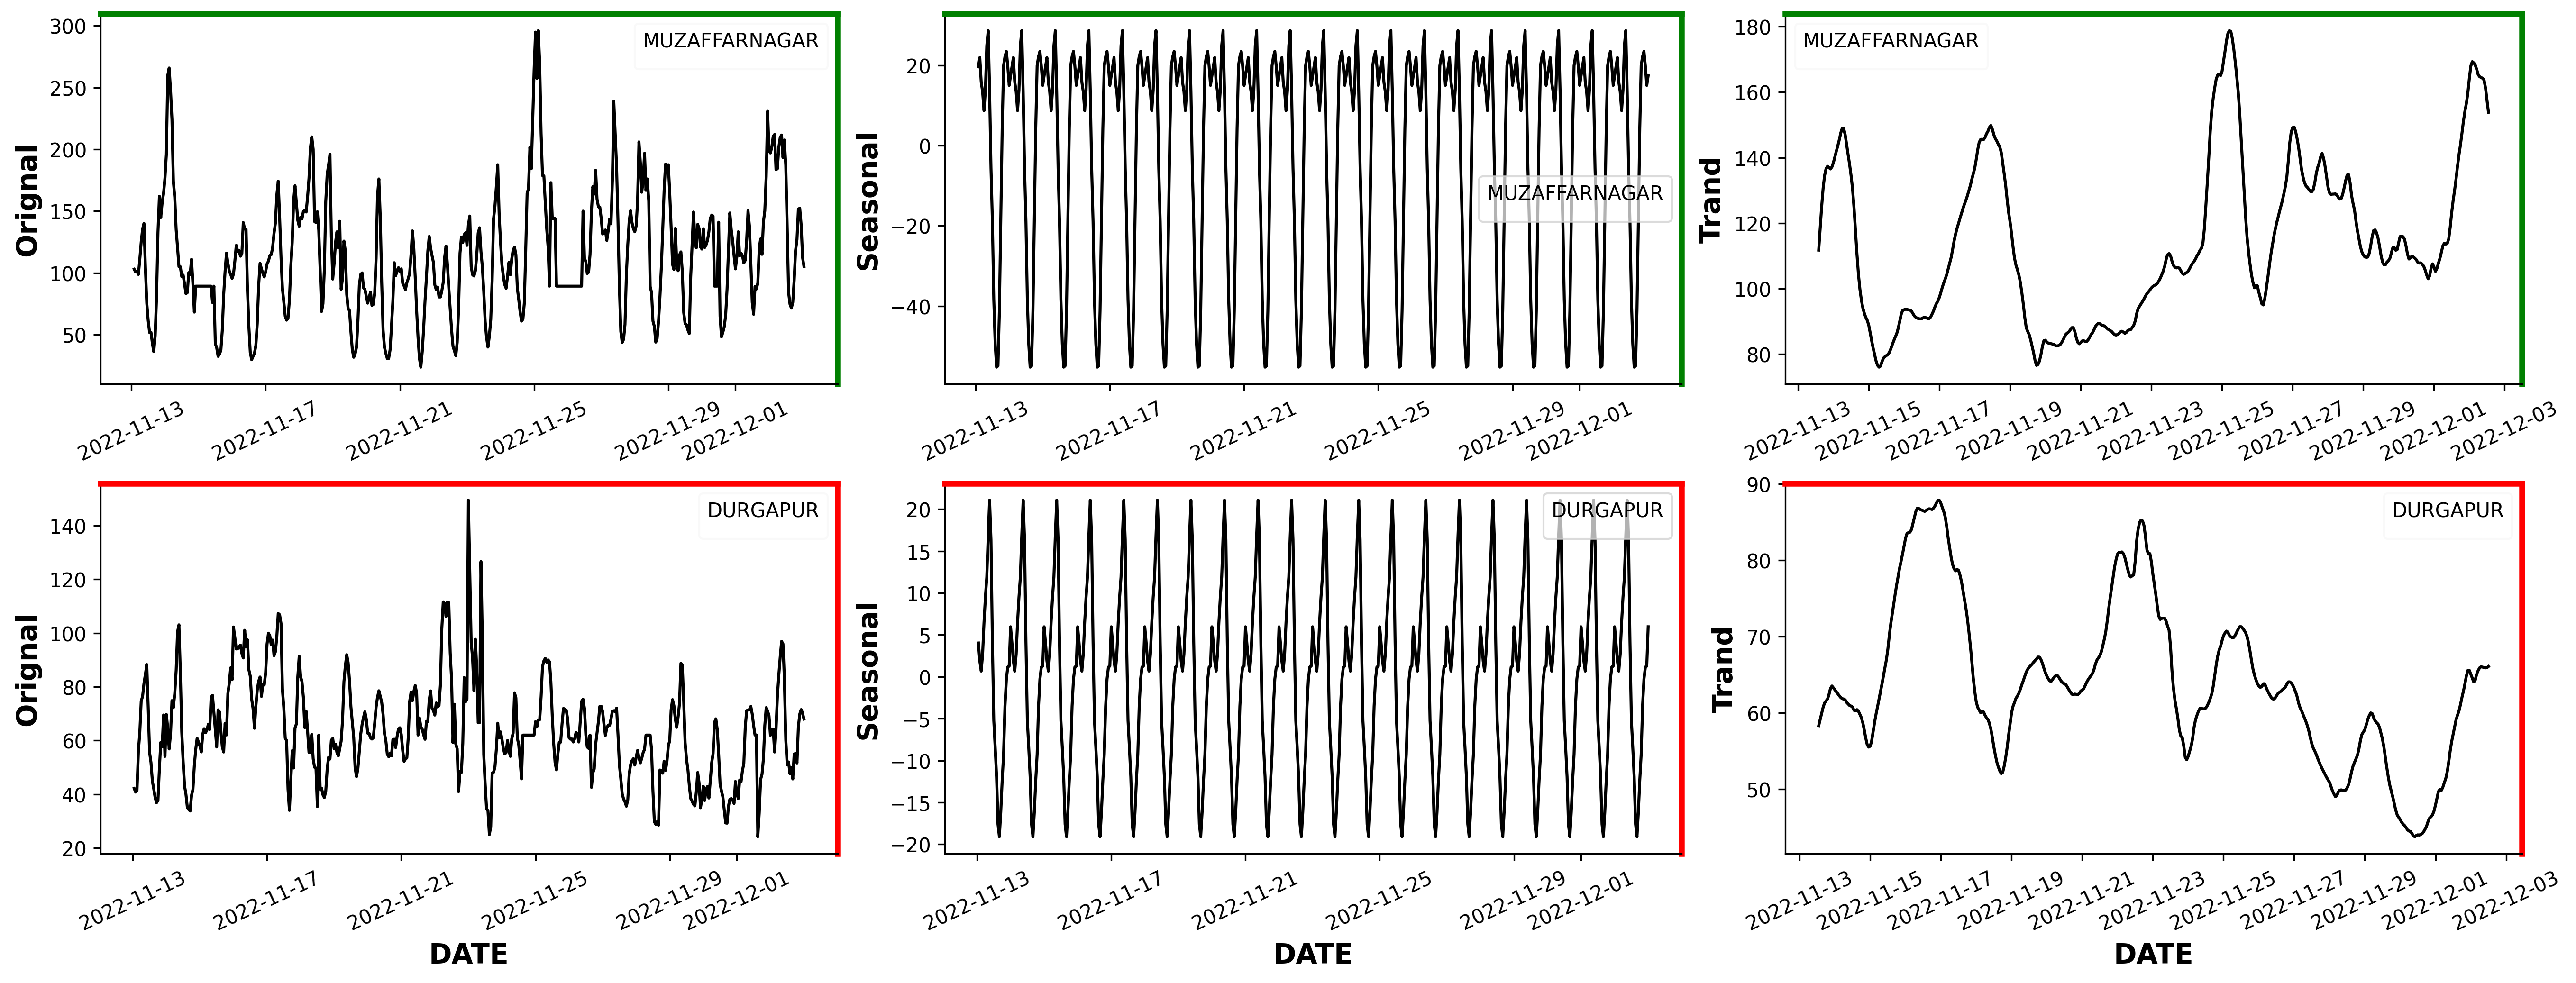
\includegraphics[scale=.2]{4}\\
	\scriptsize{FIGURE 4.5: Continuation of decomposition of 17 data sets based on trend, seasonal, and original dataset.}
\end{frame}
%\begin{frame}{Dataset Description \tiny{Continue...}}
%	\centering
%	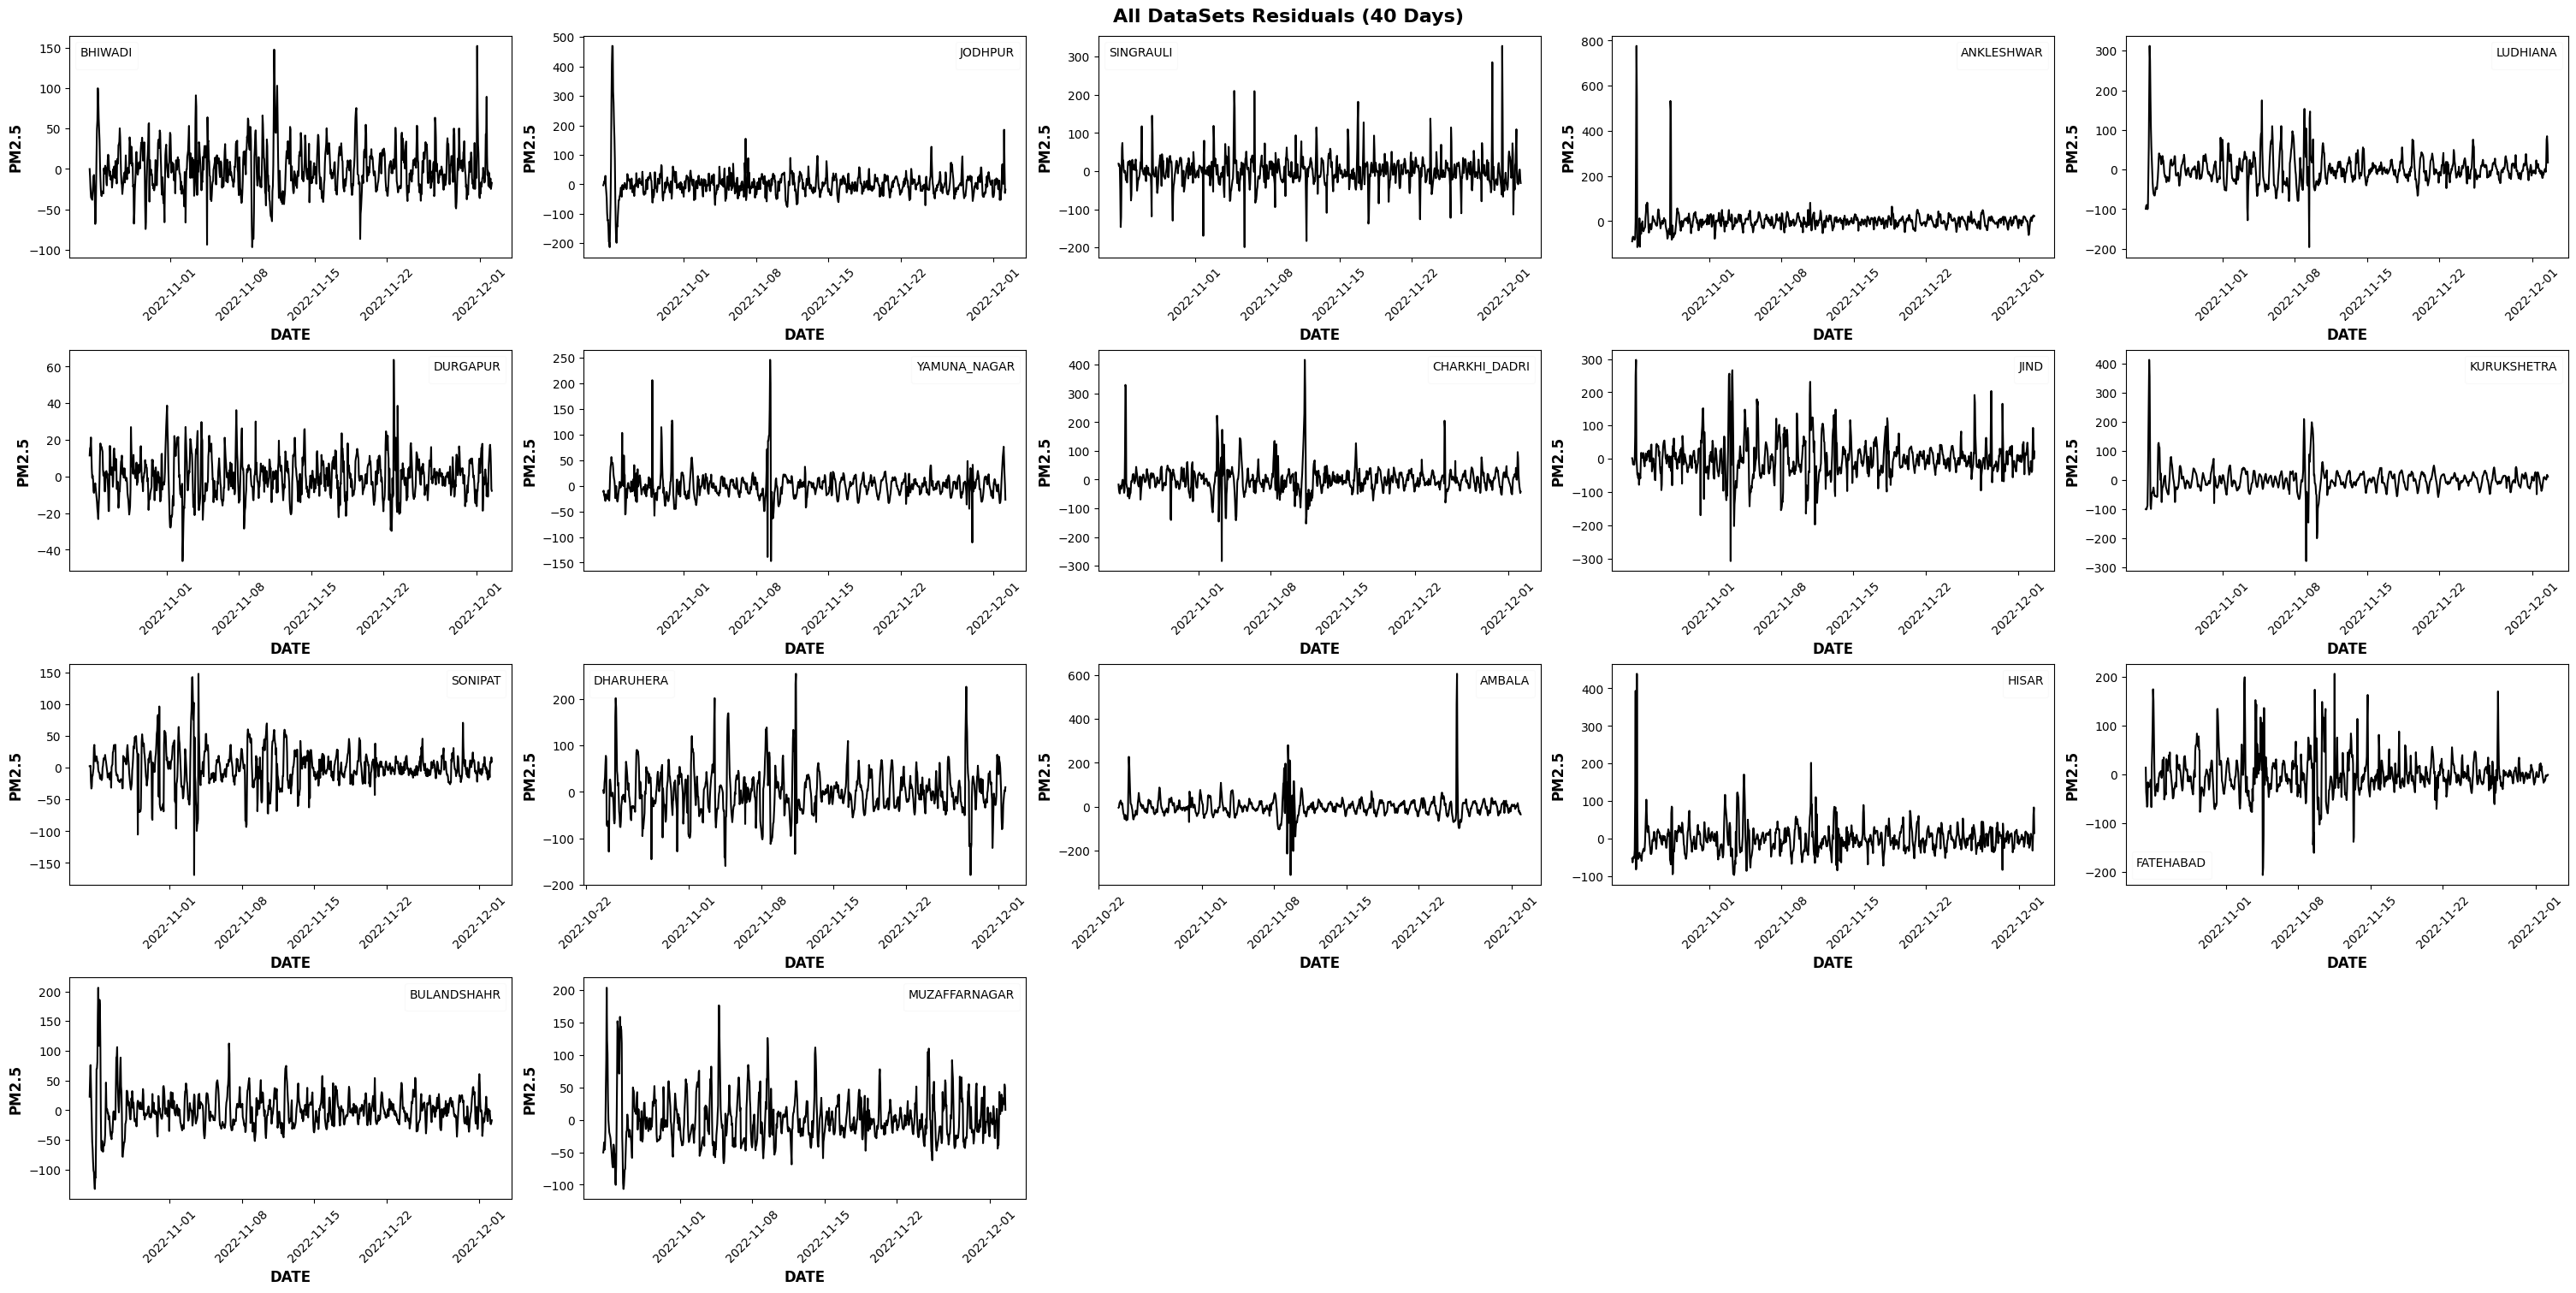
\includegraphics[scale=.18]{Residuals}\\
%	\scriptsize{FIGURE 4.5: 40 Days Residuals Graph.}
%\end{frame}


\begin{frame}{Flowchart}
	\centering
	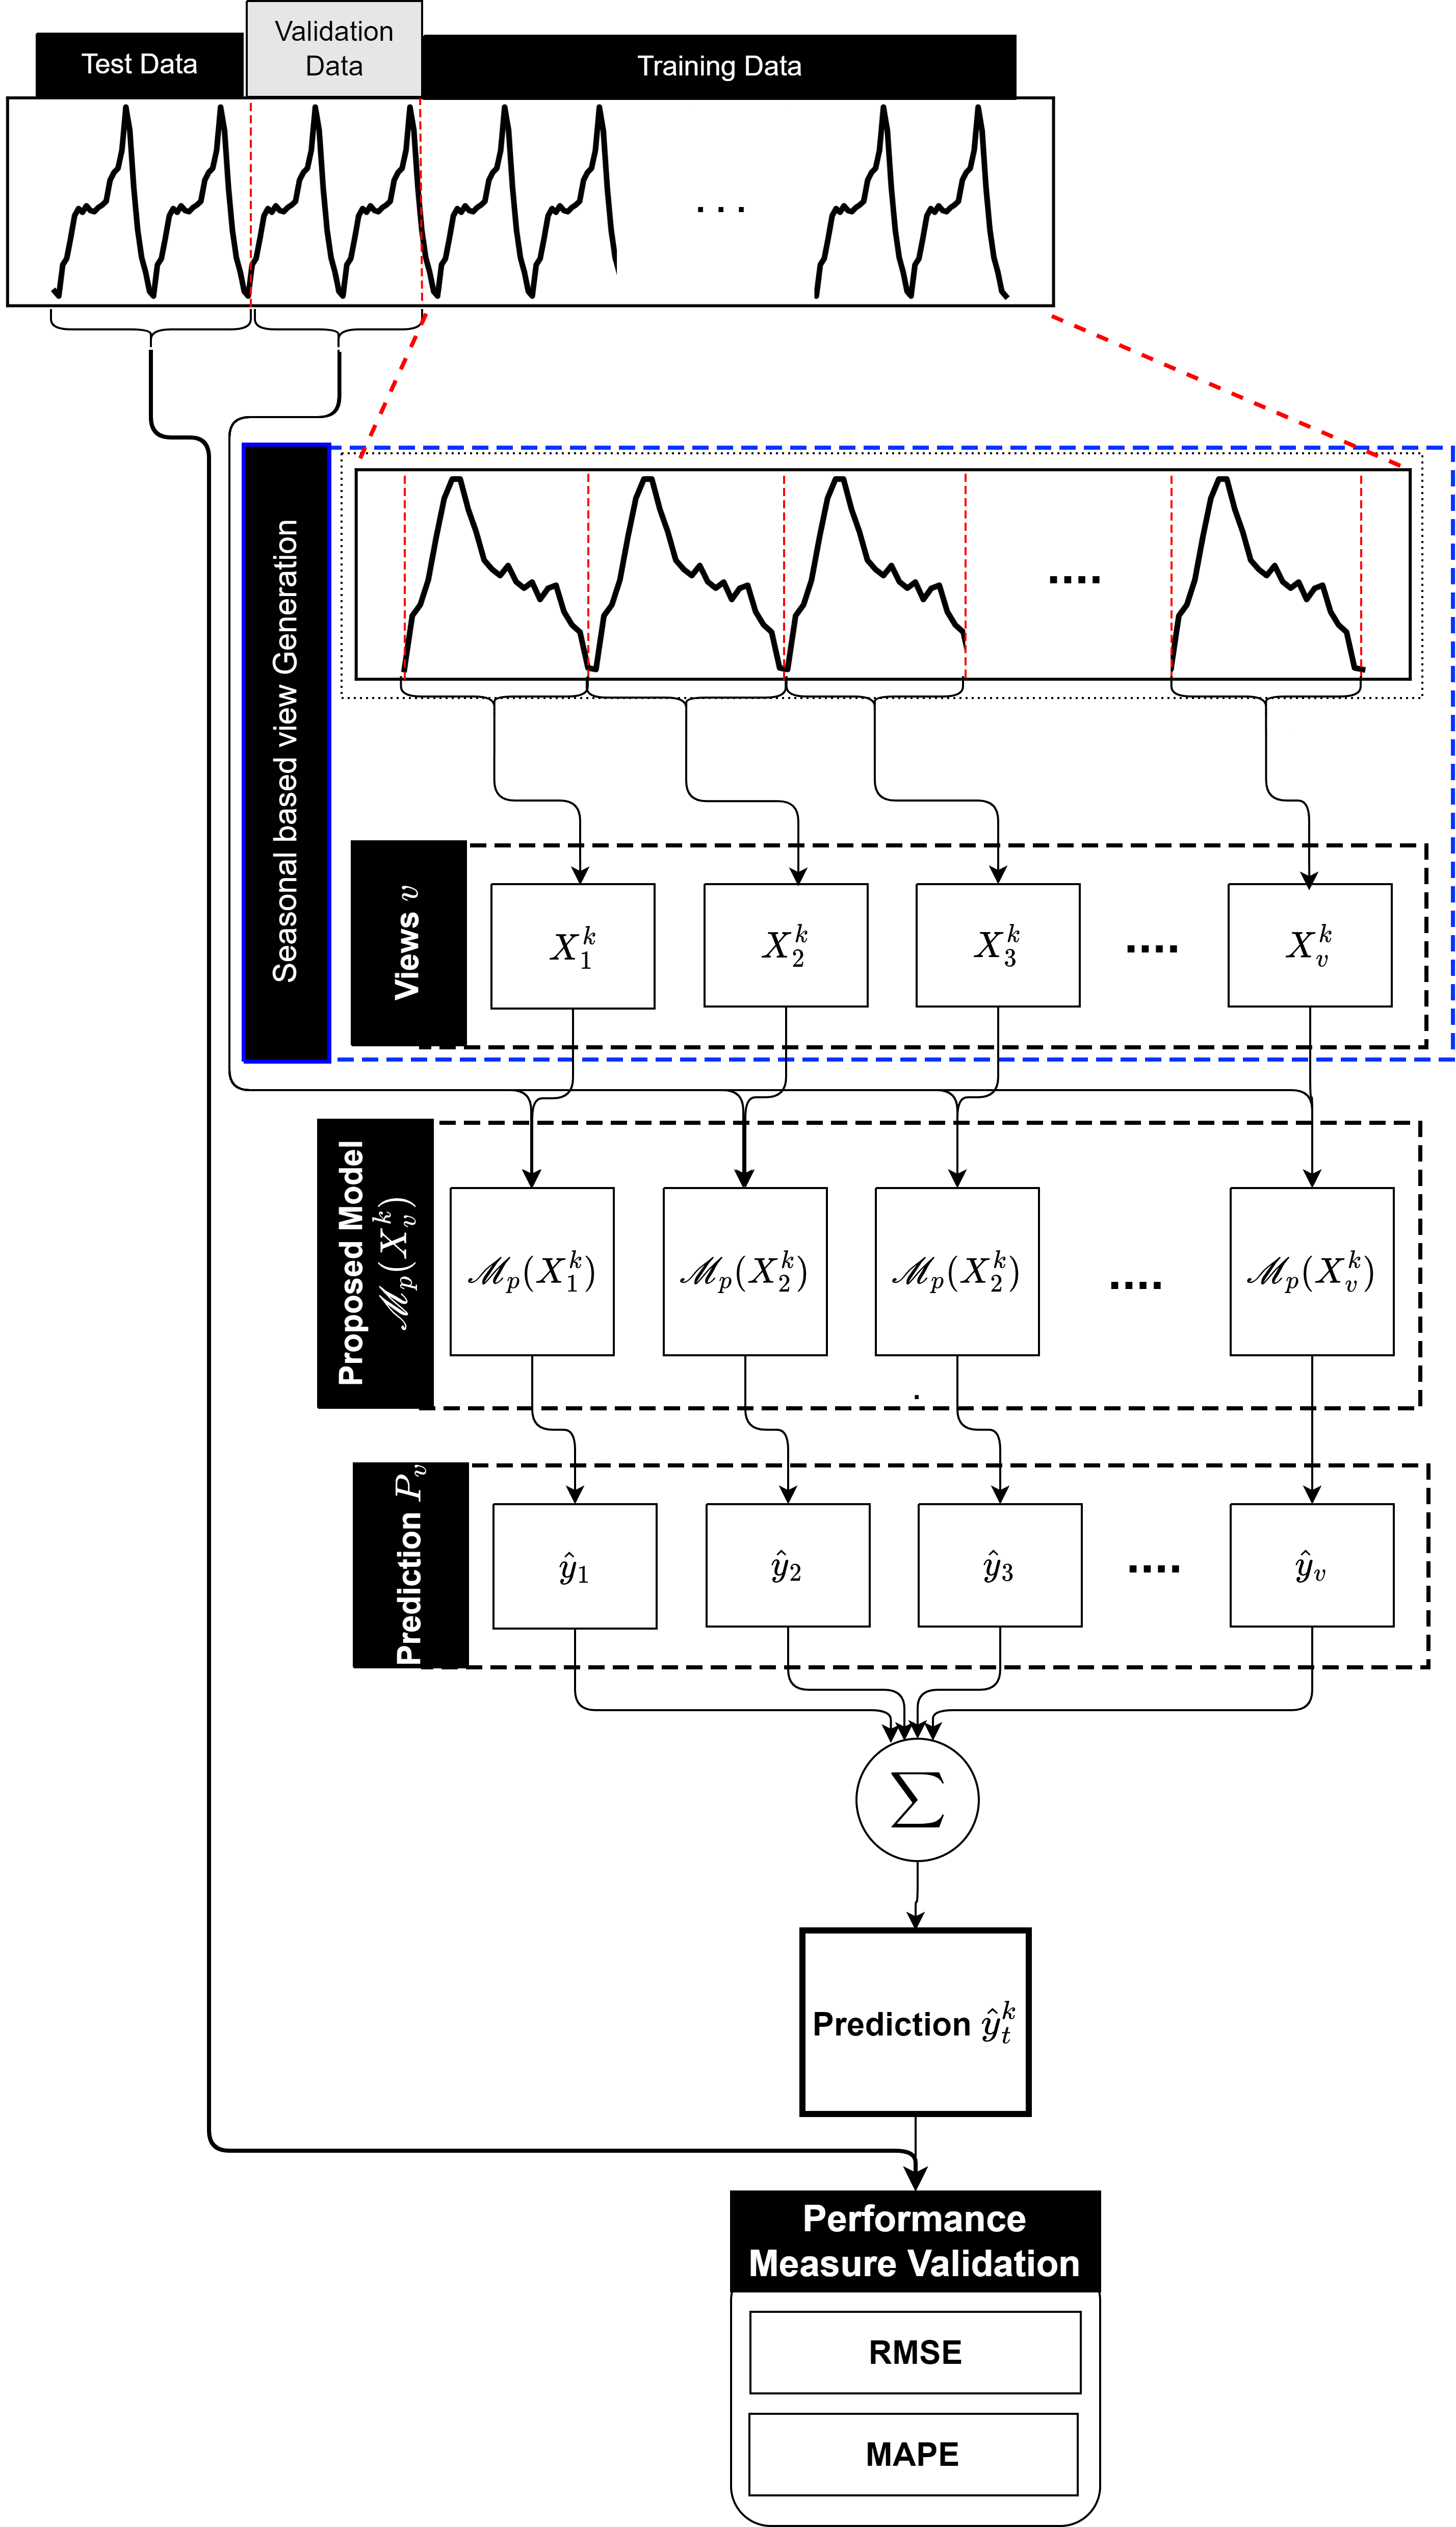
\includegraphics[scale=.2]{MvS CNN-BiLSTM.png}\\
	\scriptsize{FIGURE 4.6: Flow diagram of proposed Multi-view Stacked CNNBiLSTM (MvS CNN-BiLSTM)}
\end{frame}
\begin{frame}{Flowchart  \tiny{Continue...}}
	\centering
	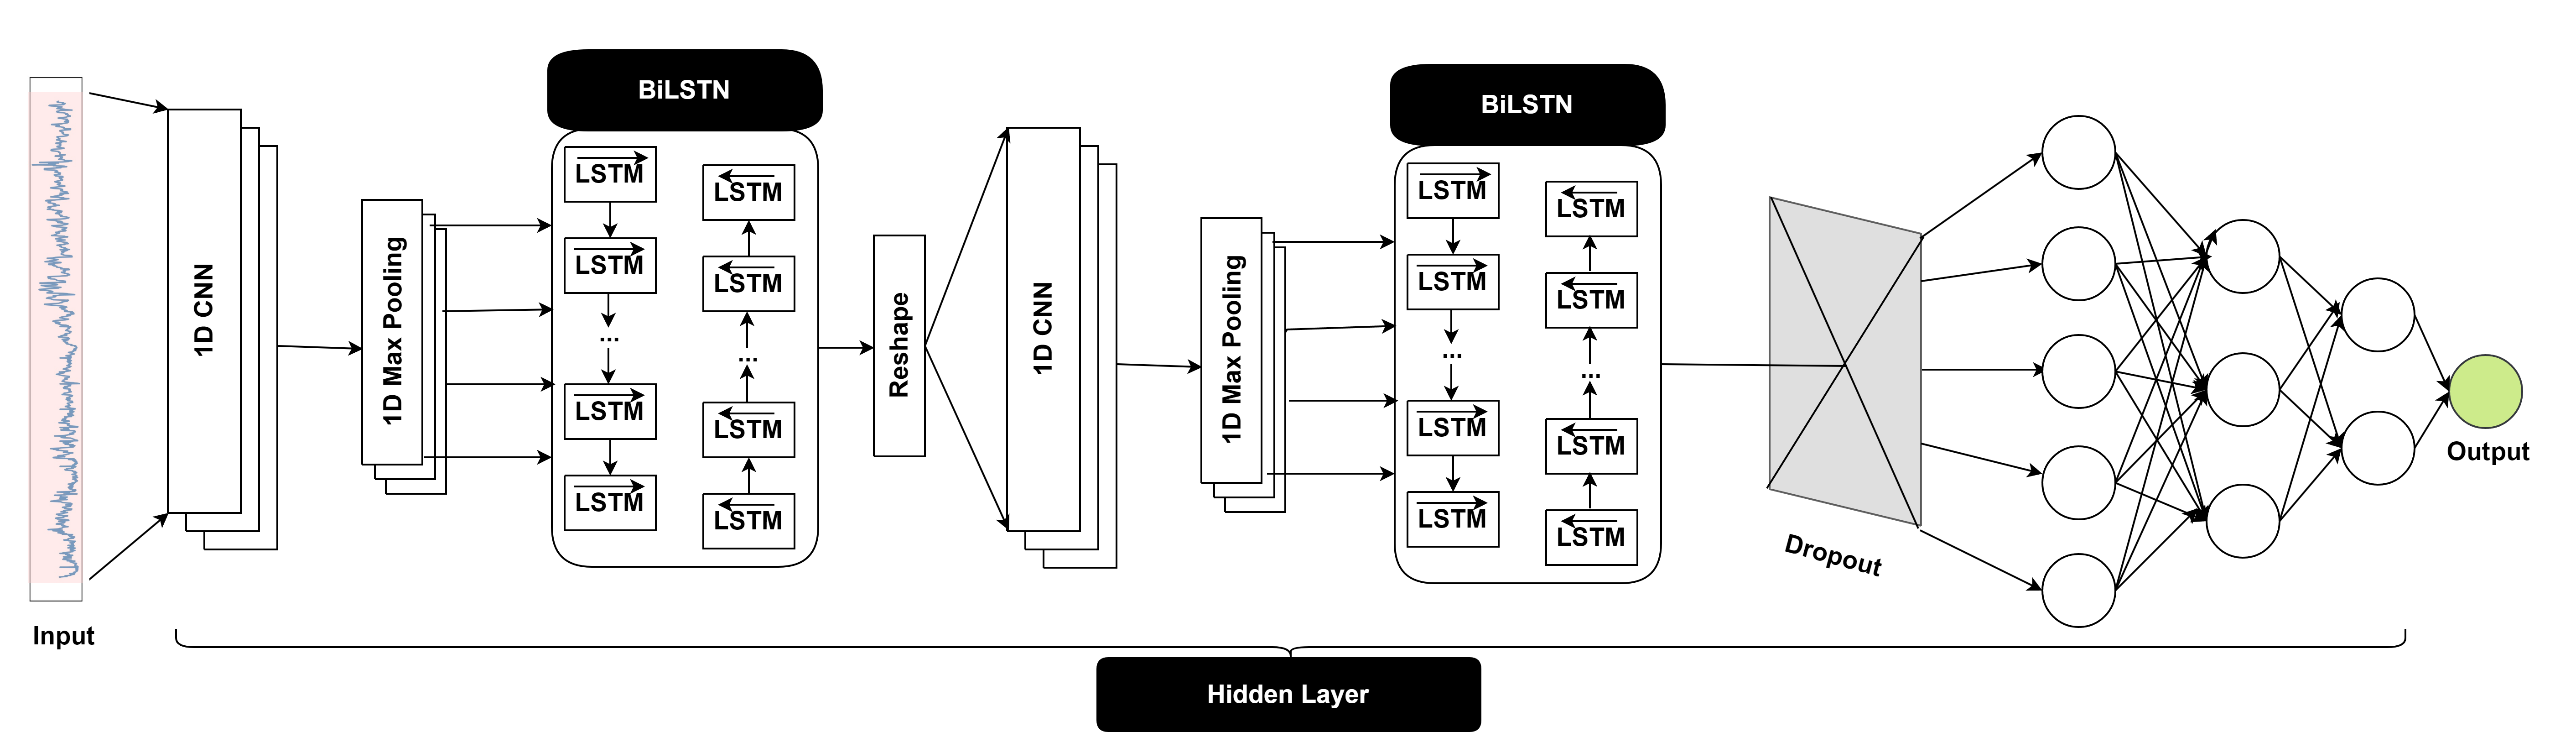
\includegraphics[scale=.4]{Prpose.png}\\
	\scriptsize{FIGURE 4.7: Architecture of Stacked CNN-BiLSTM}
\end{frame}


\begin{frame}{Hyperparameter Settings}
	\centering
	\scriptsize {TABLE 4.2:  Parameter setting of traditional DL models and proposed
	MvS CNN-BiLSTM}\\
	\begin{table}
		\begin{tabular}{|p{0.2\linewidth}|p{0.3\linewidth}|}
			\hline
			\footnotesize \textbf{Hyperparameter} & \footnotesize \textbf{Values} \\ \hline
			Batch Size               & 66                     \\ \hline
			Optimizer                 & Adam                   \\ \hline
			Loss function            & Mean Squared Error      \\ \hline
			Epoch                    & 250 with early stopping \\ \hline
			activation function      & ReLU                   \\ \hline
			training size             & 0.8                   \\ \hline
		\end{tabular}
	\end{table}
\end{frame}



%--------------------------------------------------------------------------
\section[Results and Analysis]{Results and Analysis}
%-------------------------------------------------------------------------
\begin{frame}{Results and Analysis}
	\centering
	\scriptsize {TABLE 5.1: RMSE Performance of traditional DL models and proposed models $($ MvS CNN-BiLSTM$)$.}\\
	\begin{table}
		\begin{tabular}[c]{|p{0.165\linewidth}|p{0.096\linewidth}|p{0.044\linewidth}|p{0.044\linewidth}|p{0.06\linewidth}|p{0.044\linewidth}|p{0.206\linewidth}|p{0.08\linewidth}|} \hline
		\footnotesize \textbf{DataSets} &\footnotesize  \textbf{ BiLSTM } &\footnotesize  \textbf{CNN} &\footnotesize  \textbf{GRU} &\footnotesize  \textbf{LSTM } &\footnotesize  \textbf{RNN} & \footnotesize  \textbf{MvS CNN-BiLSTM } & \footnotesize  \textbf{B-view} \\ \hline
		AMBALA         & 33.382          & 36.239    & \textbf{33.012} & 33.136     & 33.455                & 33.272          & 4      \\ \hline
		ANKLESHWAR     & 22.916          & 23.724    & 22.975          & 23.359     & 22.807                & \textbf{22.081} & 6      \\ \hline
		BHIWADI        & 28.043          & 25.168    & 25.521          & 26.512     & 25.974                & \textbf{24.959} & 10     \\ \hline
		BULANDSHAHR    & 16.155          & 16.894    & \textbf{14.807} & 16.001     & 14.923                & 16.265          & 7      \\ \hline
		 DCHARKHI\_DADRI & \textbf{30.071} & 32.709    & 32.299          & 32.629     & 33.836              & 31.064          & 3      \\ \hline
		 DHARUHERA      & 25.751          & 26.948    & 26.057          & 26.108     & 25.489           &\textbf{24.983}          & 3      \\ \hline
		 DURGAPUR       & 10.426          & 9.719     & 11.375          & 11.994     & 10.664                    & \textbf{8.906}  & 6      \\ \hline
		 FATEHABAD      & 31.501          & 31.251    & 32.169          & 31.045     & 30.946                    & \textbf{30.86}  & 10     \\ \hline
		 HISAR          & 21.677          & 22.286    & 20.875          & 21.371     & 21.617                 & \textbf{20.155} & 6      \\ \hline
		 JIND           & 26.619          & 26.29     & 25.043          & 24.813     & \textbf{24.364}           & 24.408          & 10     \\ \hline
		 JODHPUR        & 27.749          & 27.617    & 27.787          & 27.519     & 27.951              & \textbf{27.482} & 7      \\ \hline
		 KURUKSHETRA    & 16.475          & 16.352    & 15.239          & 17.359     & \textbf{15.414}           & 15.921          & 5      \\ \hline
		 LUDHIANA       & 14.573          & 17.013    & \textbf{13.817} & 17.668     & 14.936                    & 14.315          & 9      \\ \hline
		 MUZAFFARNAGAR  & 20.885          & 23.182    & 21.206          & 20.412     & 23.638                   & \textbf{19.859} & 10     \\ \hline
		 SINGRAULI      & 33.995          & 36.569    & \textbf{32.993} & 33.142     & 35.572                    & 33.834          & 2      \\ \hline
		 SONIPAT        & 13.644          & 13.951    & 14.025          & 13.773     & 13.755                    & \textbf{12.75}  & 5      \\ \hline
		 YAMUNA\_NAGAR  & 31.985          & 36.433    & 32.413          & 32.699     & 35.591                    & \textbf{31.676} & 8     \\ \hline 
		\end{tabular}
	\end{table}
\end{frame}

\begin{frame}{Results and Analysis \tiny{Continue...}}
	\centering
	\scriptsize{TABLE 5.2: Percentage improvement of MvS CNN-BiLSTM respectively BiLSTM,  CNN,  GRU,  LSTM and RNN on RMSE.}
	\begin{table}
        \begin{tabular}{ |p{0.19\linewidth} |p{0.08\linewidth} |p{0.08\linewidth} |p{0.08\linewidth} | p{0.08\linewidth} |p{0.08\linewidth}|}%{|l|l|l|l|} 
		\hline \scriptsize Dataset        & \scriptsize   BiLSTM & \scriptsize   CNN & \scriptsize  GRU & \scriptsize   LSTM & \scriptsize   RNN \\ \hline
       \scriptsize AMBALA & \scriptsize 0.33\% & \scriptsize 8.19\% & \scriptsize -0.79 \% & \scriptsize -0.41\% & \scriptsize 0.55\% \\ \hline
       \scriptsize ANKLESHWAR & \scriptsize 3.64\% & \scriptsize 6.93\% & \scriptsize 3.89\% & \scriptsize 5.47\% & \scriptsize 3.18\% \\ \hline
       \scriptsize BHIWADI & \scriptsize 11.00\% & \scriptsize 0.83\% & \scriptsize 2.20\% & \scriptsize 5.86\% & \scriptsize 3.91\% \\ \hline
       \scriptsize BULANDSHAHR & \scriptsize -0.68\% & \scriptsize 3.72\% & \scriptsize -9.85\% & \scriptsize -1.65\% & \scriptsize  -8.99\% \\ \hline
       \scriptsize CHARKHI\_DADRI & \scriptsize -3.3\% & \scriptsize  5.03\% & \scriptsize  3.82\% & \scriptsize  4.80\% & \scriptsize  8.19\% \\ \hline
       \scriptsize DHARUHERA & \scriptsize  2.98\% & \scriptsize  7.29\% & \scriptsize  4.12\% & \scriptsize  4.31\% & \scriptsize  1.99\% \\ \hline
       \scriptsize DURGAPUR & \scriptsize  14.58\% & \scriptsize  8.37\% & \scriptsize  21.71\% & \scriptsize  25.75\% & \scriptsize  16.49\% \\ \hline
       \scriptsize FATEHABAD & \scriptsize  2.03\% & \scriptsize  1.25\% & \scriptsize  4.07\% & \scriptsize  0.60\% & \scriptsize  0.28\% \\ \hline
       \scriptsize HISAR & \scriptsize  7.02\% & \scriptsize  9.56\% & \scriptsize  3.45\% & \scriptsize  5.69\% & \scriptsize  6.76\% \\ \hline
       \scriptsize JIND & \scriptsize  8.31\% & \scriptsize  7.16\% & \scriptsize  2.54\% & \scriptsize  1.63\% & \scriptsize  -0.18\% \\ \hline
       \scriptsize JODHPUR & \scriptsize  0.96\% & \scriptsize  0.49\% & \scriptsize  1.10\% & \scriptsize  0.13\% & \scriptsize  1.68\% \\ \hline
       \scriptsize KURUKSHETRA & \scriptsize  3.36\% & \scriptsize  2.64\% & \scriptsize  -4.48\% & \scriptsize  8.28\% & \scriptsize  -3.29\% \\ \hline
       \scriptsize LUDHIANA & \scriptsize  1.77\% & \scriptsize  15.86\% & \scriptsize  -3.6\% & \scriptsize  18.98\% & \scriptsize  4.16\% \\ \hline
       \scriptsize MUZAFFARNAGAR & \scriptsize  4.91\% & \scriptsize  14.33\% & \scriptsize  6.35\% & \scriptsize  2.71\% & \scriptsize  15.99\% \\ \hline
       \scriptsize SINGRAULI & \scriptsize  0.47\% & \scriptsize  7.48\% & \scriptsize  -2.55\% & \scriptsize  -2.09\% & \scriptsize  4.89\% \\ \hline
       \scriptsize SONIPAT & \scriptsize  6.55\% & \scriptsize  8.61\% & \scriptsize  9.09\% & \scriptsize  7.43\% & \scriptsize  7.31\% \\ \hline
       \scriptsize YAMUNA\_NAGAR & \scriptsize  0.97\% & \scriptsize  13.06\% & \scriptsize  2.27\% & \scriptsize  3.13\% & \scriptsize  11.00\% \\ \hline 
       \scriptsize \textbf{Positive Avg}  & \scriptsize  \textbf{4.05\%} & \scriptsize  \textbf{7.11\%}& \scriptsize  \textbf{3.80\%} & \scriptsize  \textbf{5.57\%} & \scriptsize  \textbf{5.08\%} \\ \hline
        \end{tabular}
    \end{table}
\end{frame}

\begin{frame}{Results and Analysis  \tiny{Continue...}}
	\centering
	\scriptsize {TABLE 5.3: MAPE Performance of traditional DL models and proposed models $($MvS CNN-BiLSTM$)$.}\\
	\begin{table}
		\begin{tabular}[c]{|p{0.165\linewidth}|p{0.096\linewidth}|p{0.044\linewidth}|p{0.044\linewidth}|p{0.06\linewidth}|p{0.044\linewidth}|p{0.206\linewidth}|p{0.08\linewidth}|} \hline
		\footnotesize \textbf{DataSets} &\footnotesize  \textbf{ BiLSTM } &\footnotesize  \textbf{CNN} &\footnotesize  \textbf{GRU} &\footnotesize  \textbf{LSTM } &\footnotesize  \textbf{RNN} & \footnotesize  \textbf{MvS CNN-BiLSTM } & \footnotesize  \textbf{B-view} \\ \hline
		AMBALA         & 54.468       & 49.153    & 76.839    & 58.619     & 53.375    & \textbf{18.73}  & 3      \\ \hline
		ANKLESHWAR     & 18.86        & 19.968    & 19.015    & 19.576     & 20.72     & \textbf{16.265} & 10     \\ \hline
		BHIWADI        & 134.448      & 118.741   & 123.123   & 127.481    & 124.503   & \textbf{20.98}  & 2      \\ \hline
		BULANDSHAHR    & 44.602       & 47.066    & 26.254    & 43.721     & 27.813    & \textbf{22.469} & 3      \\ \hline
		CHARKHI\_DADRI & 50.328       & 101.385   & 102.063   & 112.912    & 115.673   & \textbf{26.728} & 10     \\ \hline
		DHARUHERA      & 35.638       & 39.358    & 39.557    & 35.942     & 40.34     & \textbf{17.365} & 3      \\ \hline
		DURGAPUR       & 45.511       & 37.529    & 56.324    & 57.457     & 48.626    & \textbf{19.321} & 6      \\ \hline
		FATEHABAD      & 19.737       & 19.929    & 19.475    & 18.663     & 17.724    & \textbf{12.178} & 5      \\ \hline
		HISAR          & 17.971       & 18.422    & 17.988    & 17.983     & 21.475    & \textbf{15.082} & 6      \\ \hline
		JIND           & 25.945       & 30.822    & 27.344    & 24.596     & 33.464    & \textbf{16.618} & 3      \\ \hline
		JODHPUR        & 40.188       & 40.36     & 41.584    & 41.578     & 43.36     & \textbf{28.278} & 7      \\ \hline
		KURUKSHETRA    & 13.713       & 13.392    & 12.405    & 13.986     & 13.312    & \textbf{11.248} & 2      \\ \hline
		LUDHIANA       & 37.61        & 47.14     & 34.504    & 51.036     & 41.197    & \textbf{15.706} & 9      \\ \hline
		MUZAFFARNAGAR  & 24.162       & 27.253    & 23.37     & 26.08      & 27.061    & \textbf{16.571} & 5      \\ \hline
		SINGRAULI      & 48.642       & 67.143    & 39.738    & 34.372     & 68.525    & \textbf{28.545} & 7      \\ \hline
		SONIPAT        & 43.301       & 48.32     & 49.409    & 43.187     & 45.67     & \textbf{13.541} & 7      \\ \hline
		YAMUNA\_NAGAR  & 65.601       & 63.698    & 64.637    & 63.404     & 70.02     & \textbf{28.29}  & 10    \\ \hline
		\end{tabular}
	\end{table}
\end{frame}

\begin{frame}{Results and Analysis \tiny{Continue...}}
	\centering
	\scriptsize{TABLE 5.4: Improvement of MvS CNN-BiLSTM respectively BiLSTM,  GRU,  LSTM and RNN on MAPE.}
	\begin{table}
        \begin{tabular}{ |p{0.19\linewidth} |p{0.08\linewidth} |p{0.08\linewidth} |p{0.08\linewidth} | p{0.08\linewidth} |p{0.08\linewidth}|}%{|l|l|l|l|} 
		\hline \scriptsize Dataset        & \scriptsize   BiLSTM & \scriptsize   CNN & \scriptsize  GRU & \scriptsize   LSTM & \scriptsize   RNN \\ \hline
		\scriptsize AMBALA & \scriptsize 35.74\% & \scriptsize 30.42\% & \scriptsize 58.11\% & \scriptsize 39.89\% & \scriptsize 34.64\% \\ \hline
		\scriptsize ANKLESHWAR & \scriptsize 2.59\% & \scriptsize 3.70\% & \scriptsize 2.75\% & \scriptsize 3.31\% & \scriptsize 4.45\% \\ \hline
		\scriptsize BHIWADI & \scriptsize 113.47\% & \scriptsize 97.76\% & \scriptsize 102.14\% & \scriptsize 106.50\% & \scriptsize 103.52\% \\ \hline
		\scriptsize BULANDSHAHR & \scriptsize 22.13\% & \scriptsize 24.60\% & \scriptsize 3.78\% & \scriptsize 21.25\% & \scriptsize 5.34\% \\ \hline
		\scriptsize CHARKHI\_DADRI & \scriptsize 23.60\% & \scriptsize 74.66\% & \scriptsize 75.34\% & \scriptsize 86.18\% & \scriptsize 88.94\% \\ \hline
		\scriptsize DHARUHERA & \scriptsize 18.27\% & \scriptsize 21.99\% & \scriptsize 22.19\% & \scriptsize 18.58\% & \scriptsize 22.98\% \\ \hline
		\scriptsize DURGAPUR & \scriptsize 26.19\% & \scriptsize 18.21\% & \scriptsize 37.00\% & \scriptsize 38.14\% & \scriptsize 29.30\% \\ \hline
		\scriptsize FATEHABAD & \scriptsize 7.56\% & \scriptsize 7.75\% & \scriptsize 7.30\% & \scriptsize 6.48\% & \scriptsize 5.55\% \\ \hline
		\scriptsize HISAR & \scriptsize 2.89\% & \scriptsize 3.34\% & \scriptsize 2.91\% & \scriptsize 2.90\% & \scriptsize 6.39\% \\ \hline
		\scriptsize JIND & \scriptsize 9.33\% & \scriptsize 14.20\% & \scriptsize 10.73\% & \scriptsize 7.98\% & \scriptsize 16.85\% \\ \hline
		\scriptsize JODHPUR & \scriptsize 11.91\% & \scriptsize 12.08\% & \scriptsize 13.31\% & \scriptsize 13.30\% & \scriptsize 15.08\% \\ \hline
		\scriptsize KURUKSHETRA & \scriptsize 2.46\% & \scriptsize 2.14\% & \scriptsize 1.16\% & \scriptsize 2.74\% & \scriptsize 2.06\% \\ \hline
		\scriptsize LUDHIANA & \scriptsize 21.90\% & \scriptsize 31.43\% & \scriptsize 18.80\% & \scriptsize 35.33\% & \scriptsize 25.49\% \\ \hline
		\scriptsize MUZAFFARNAGAR & \scriptsize 7.59\% & \scriptsize 10.68\% & \scriptsize 6.80\% & \scriptsize 9.51\% & \scriptsize 10.49\% \\ \hline
		\scriptsize SINGRAULI & \scriptsize 20.10\% & \scriptsize 38.60\% & \scriptsize 11.19\% & \scriptsize 5.83\% & \scriptsize 39.98\% \\ \hline
		\scriptsize SONIPAT & \scriptsize 29.76\% & \scriptsize 34.78\% & \scriptsize 35.87\% & \scriptsize 29.65\% & \scriptsize 32.13\% \\ \hline
		\scriptsize YAMUNA\_NAGAR & \scriptsize 37.31\% & \scriptsize 35.41\% & \scriptsize 36.35\% & \scriptsize 35.11\% & \scriptsize 41.73\% \\ \hline
		\scriptsize \textbf{Positive Avg} & \scriptsize \textbf{23.11\% }& \scriptsize \textbf{27.16\% }& \scriptsize \textbf{26.22\%} & \scriptsize \textbf{27.22\%} & \scriptsize \textbf{28.52\%} \\ \hline
		\end{tabular}
    \end{table}
\end{frame}




% \iffalse
% \begin{frame}{Results and Analysis \tiny{Continue...}}
% 	\centering
% 	\scriptsize {TABLE 5.2: Average Rankings of RMSE by (N*N) Friedman Test}\\
% 	\begin{table}
% 		\centering
% 		\begin{tabular}{|p{0.2\linewidth}|p{0.1\linewidth}|}
% 			\hline
% 			\footnotesize \textbf{Algorithm} & \footnotesize \textbf{Ranking} \\ \hline
% 			BiLSTM & 2.1176\\ \hline
% 			CNN & 4.2941\\\hline
% 			GRU & 5.7059\\\hline
% 			Seq2Seq & 3.1176\\\hline
% 			V-LSTM & 1.7059\\\hline
% 			S-LSTM & 7.1176\\\hline
% 			CNN-BiLSTM & 6.5294\\\hline
% 			CNN-LSTM & 6.9412\\\hline
% 			GRU-BiLSTM & 7.4706\\\hline
% 		\end{tabular}
% 	\end{table}
% \end{frame}
% \fi



% \begin{frame}{Results and Analysis \tiny{Continue...}}
% 	\centering
% 	\scriptsize {TABLE 5.3: \textbf{MAE} Acrose Models on 17 Indian Cities Dataset.}\\
% 	\begin{table}
% 		\begin{tabular}{|p{0.165\linewidth}|p{0.04\linewidth}|p{0.04\linewidth}|p{0.04\linewidth}|p{0.04\linewidth}|p{0.05\linewidth}|p{0.05\linewidth}|p{0.08\linewidth}|p{0.05\linewidth}|p{0.08\linewidth}|} \hline
% 		\footnotesize \textbf{DataSets} &\footnotesize  \textbf{BiLS- TM} &\footnotesize  \textbf{CNN} &\footnotesize  \textbf{GRU} &\footnotesize  \textbf{Seq2- Seq} &\footnotesize  \textbf{V-LSTM} & \footnotesize  \textbf{S-LSTM} & \footnotesize \textbf{CNN\_Bi-LSTM} &\footnotesize  \textbf{CNN\_ LSTM} &\footnotesize  \textbf{GRU\_Bi-LSTM} \\ \hline
% 		\textbf{BHIWADI}        & 16.61 & 53.94 & 15.58 & 17.05 & 12.35 & 34.31 & 39.66 & 40.3  & 23.06 \\ \hline
% 		\textbf{JODHPUR}        & 19.71 & 20.2  & 24.93 & 17.51 & 14.3  & 35.72 & 29.35 & 32.47 & 38.12 \\ \hline
% 		\textbf{SINGRAULI}      & 7.02  & 10.49 & 25.99 & 19.48 & 11.79 & 13.18 & 49.16 & 20.97 & 24.55 \\ \hline
% 		\textbf{ANKLESHWAR}     & 13.3  & 12.17 & 30.31 & 18.87 & 13.78 & 37.08 & 51.31 & 57.53 & 58.27 \\ \hline
% 		\textbf{LUDHIANA}       & 6.13  & 9.05  & 17.5  & 7.73  & 6.95  & 15.97 & 20.93 & 19.84 & 18.03 \\ \hline
% 		\textbf{DURGAPUR}       & 4.47  & 6.23  & 19.32 & 7.38  & 7.81  & 11.75 & 7.32  & 12.6  & 21.97 \\ \hline
% 		\textbf{YAMUNA\_NAGAR}  & 17.05 & 17.73 & 31.74 & 15.11 & 17.86 & 39.13 & 42.25 & 23.31 & 43.99 \\ \hline
% 		\textbf{CHARKHI\_DADRI} & 11.66 & 14.52 & 19.91 & 11.38 & 11.24 & 30.32 & 35    & 33.34 & 33    \\ \hline
% 		\textbf{JIND}           & 15.28 & 17.46 & 23.74 & 16.72 & 11.46 & 51.71 & 46.76 & 27.89 & 33.97 \\ \hline
% 		\textbf{KURUKSHETRA}    & 13.83 & 45.5  & 24.77 & 16.83 & 14.73 & 42.26 & 24.43 & 53.83 & 32.16 \\ \hline
% 		\textbf{SONIPAT}        & 7.05  & 9.54  & 15.09 & 9.03  & 6.26  & 26.95 & 14.68 & 13.65 & 29.12 \\ \hline
% 		\textbf{DHARUHERA}      & 11.92 & 17.22 & 17.8  & 9.62  & 10.61 & 32.7  & 16.99 & 18.8  & 25.45 \\ \hline
% 		\textbf{AMBALA}         & 13.03 & 17.01 & 22.05 & 11.21 & 8.96  & 34.42 & 24.82 & 19.51 & 37.19 \\ \hline
% 		\textbf{HISAR}          & 12.3  & 45.7  & 29.6  & 19.54 & 15.93 & 41.06 & 27.53 & 30.51 & 41.18 \\ \hline
% 		\textbf{FATEHABAD}      & 8.64  & 29.69 & 45.76 & 8.64  & 9.37  & 25.94 & 47.32 & 48.3  & 46.98 \\ \hline
% 		\textbf{BULANDSHAHR}    & 4.76  & 7.38  & 19.15 & 9.01  & 5.6   & 11.85 & 7.28  & 11.81 & 8.21  \\ \hline
% 		\textbf{MUZAFFARNAGAR}  & 8.23  & 12.65 & 11.26 & 11.68 & 10.47 & 16.65 & 12.9  & 21.33 & 18.49 \\ \hline
% 		\end{tabular}
% 	\end{table}
% \end{frame}

% \iffalse
% \begin{frame}{Results and Analysis \tiny{Continue...}}
% 	\centering
% 	\scriptsize {TABLE 5.4: Average Rankings of MAE by (N*N) Friedman Test}\\
% 	\begin{table}
% 		\centering
% 		\begin{tabular}{|p{0.2\linewidth}|p{0.1\linewidth}|}
% 			\hline
% 			\footnotesize \textbf{Algorithm} & \footnotesize \textbf{Ranking} \\ \hline
% 			BiLSTM & 1.9412\\\hline
% 			CNN & 4.4706\\\hline
% 			GRU & 5.7059\\\hline
% 			Seq2Seq & 3\\\hline
% 			V-LSTM & 2.1176\\\hline
% 			S-LSTM & 6.7647\\\hline
% 			CNN-BiLSTM & 6.3529\\\hline
% 			CNN-LSTM & 7.0588\\\hline
% 			GRU-BiLSTM & 7.5882\\\hline
% 		\end{tabular}
% 	\end{table}
% \end{frame}
% \fi

% \begin{frame}{Results and Analysis \tiny{Continue...}}
% 	\centering
% 	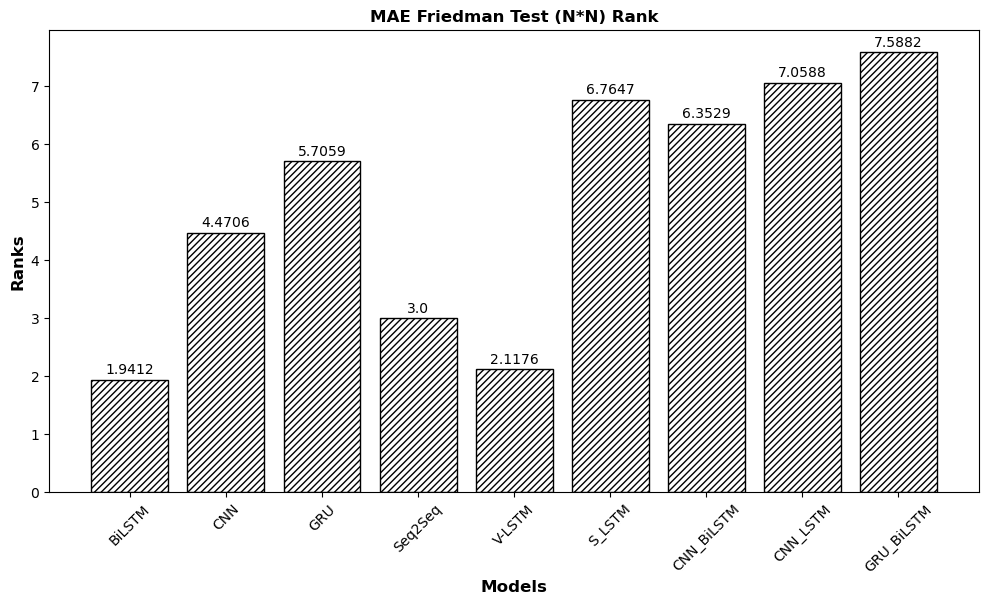
\includegraphics[scale=.45]{MAE Friedman Test (N_N) Rank}\\
% 	\scriptsize{FIGURE 5.2: Best model on (N*N) Friedman Test for \textbf{MAE}}
% \end{frame}


% \begin{frame}{Results and Analysis \tiny{Continue...}}
% 	\centering
% 	\scriptsize {TABLE 5.5: \textbf{MAPE} Acrose Models on 17 Indian Cities Dataset.}\\
% 	\begin{table}
% 		\begin{tabular}{|p{0.165\linewidth}|p{0.04\linewidth}|p{0.04\linewidth}|p{0.04\linewidth}|p{0.04\linewidth}|p{0.05\linewidth}|p{0.05\linewidth}|p{0.08\linewidth}|p{0.05\linewidth}|p{0.08\linewidth}|} \hline
% 		\footnotesize \textbf{DataSets} &\footnotesize  \textbf{BiLS- TM} &\footnotesize  \textbf{CNN} &\footnotesize  \textbf{GRU} &\footnotesize  \textbf{Seq2- Seq} &\footnotesize  \textbf{V-LSTM} & \footnotesize  \textbf{S-LSTM} & \footnotesize \textbf{CNN\_Bi-LSTM} &\footnotesize  \textbf{CNN\_ LSTM} &\footnotesize  \textbf{GRU\_Bi-LSTM} \\ \hline
% 		\textbf{BHIWADI}        & 0.43 & 1.34 & 0.48 & 0.49 & 0.35 & 0.96 & 1.11 & 1.06 & 0.63 \\ \hline
% 		\textbf{JODHPUR}        & 0.31 & 0.33 & 0.44 & 0.37 & 0.29 & 0.55 & 0.44 & 0.55 & 0.57 \\ \hline
% 		\textbf{SINGRAULI}      & 0.61 & 0.66 & 2.13 & 1.62 & 1.02 & 1.06 & 3.57 & 1.72 & 2.03 \\ \hline
% 		\textbf{ANKLESHWAR}     & 0.15 & 0.13 & 0.25 & 0.16 & 0.13 & 0.31 & 0.4  & 0.46 & 0.47 \\ \hline
% 		\textbf{LUDHIANA}       & 0.15 & 0.28 & 0.57 & 0.22 & 0.22 & 0.43 & 0.71 & 0.66 & 0.51 \\ \hline
% 		\textbf{DURGAPUR}       & 0.28 & 0.51 & 0.93 & 0.71 & 0.42 & 0.84 & 0.66 & 0.72 & 1.38 \\ \hline
% 		\textbf{YAMUNA\_NAGAR}  & 0.23 & 0.26 & 0.33 & 0.19 & 0.26 & 0.53 & 0.47 & 0.32 & 0.47 \\ \hline
% 		\textbf{CHARKHI\_DADRI} & 0.48 & 0.75 & 0.75 & 0.72 & 0.48 & 1.12 & 2.08 & 1.88 & 1.95 \\ \hline
% 		\textbf{JIND}           & 0.15 & 0.21 & 0.3  & 0.14 & 0.12 & 0.48 & 0.39 & 0.23 & 0.3  \\ \hline
% 		\textbf{KURUKSHETRA}    & 0.19 & 0.4  & 0.27 & 0.23 & 0.2  & 0.51 & 0.34 & 0.54 & 0.31 \\ \hline
% 		\textbf{SONIPAT}        & 0.16 & 0.18 & 0.36 & 0.21 & 0.14 & 0.58 & 0.33 & 0.24 & 0.38 \\ \hline
% 		\textbf{DHARUHERA}      & 0.3  & 0.58 & 0.41 & 0.33 & 0.25 & 0.87 & 0.52 & 0.38 & 0.52 \\ \hline
% 		\textbf{AMBALA}         & 0.29 & 0.48 & 0.42 & 0.26 & 0.25 & 0.87 & 0.41 & 0.49 & 0.83 \\ \hline
% 		\textbf{HISAR}          & 0.13 & 0.31 & 0.23 & 0.17 & 0.16 & 0.39 & 0.32 & 0.28 & 0.31 \\ \hline
% 		\textbf{FATEHABAD}      & 0.13 & 0.35 & 0.5  & 0.12 & 0.11 & 0.44 & 0.61 & 0.57 & 0.65 \\ \hline
% 		\textbf{BULANDSHAHR}    & 0.29 & 0.6  & 1.35 & 0.76 & 0.44 & 0.99 & 0.61 & 0.97 & 0.56 \\ \hline
% 		\textbf{MUZAFFARNAGAR}  & 0.3  & 0.62 & 0.59 & 0.67 & 0.55 & 0.68 & 0.69 & 1.11 & 0.97 \\ \hline
% 		\end{tabular}
% 	\end{table}
% \end{frame}

% \iffalse
% \begin{frame}{Results and Analysis \tiny{Continue...}}
% 	\centering
% 	\scriptsize {TABLE 5.6: Average Rankings of MAPE by (N*N) Friedman Test}\\
% 	\begin{table}
% 		\centering
% 		\begin{tabular}{|p{0.2\linewidth}|p{0.1\linewidth}|}
% 			\hline
% 			\footnotesize \textbf{Algorithm} & \footnotesize \textbf{Ranking} \\ \hline
% 			BiLSTM & 1.8235\\\hline
% 			CNN & 4.5882\\\hline
% 			GRU & 5.6471\\\hline
% 			Seq2Seq & 3.4118\\\hline
% 			V-LSTM & 1.7059\\\hline
% 			S-LSTM & 7.2353\\\hline
% 			CNN-BiLSTM & 7\\\hline
% 			CNN-LSTM & 6.5882\\\hline
% 			GRU-BiLSTM & 7\\\hline
% 		\end{tabular}
% 	\end{table}
% \end{frame}
% \fi

% \begin{frame}{Results and Analysis \tiny{Continue...}}
% 	\centering
% 	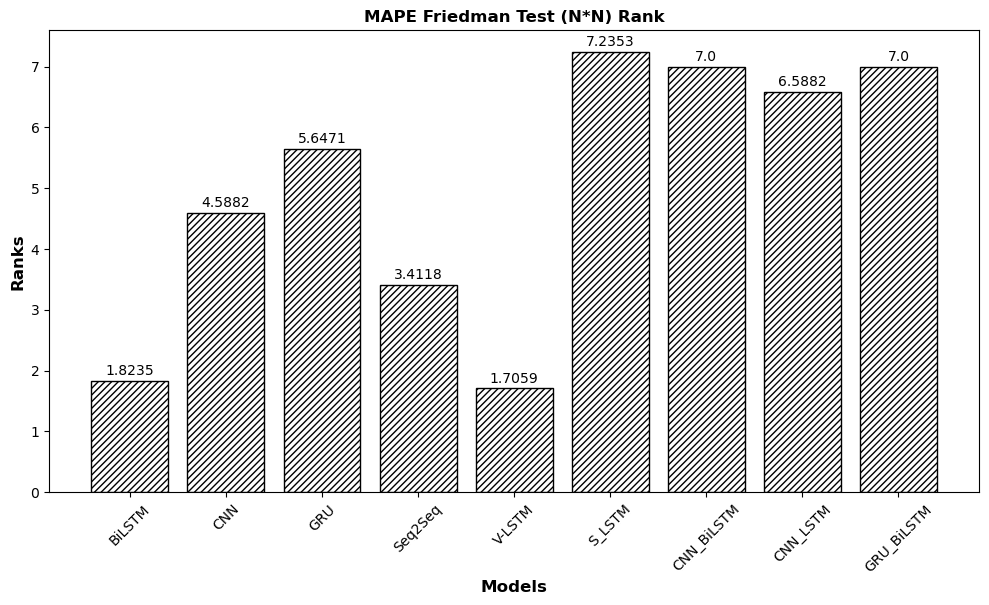
\includegraphics[scale=.45]{MAPE Friedman Test (N_N) Rank}\\
% 	\scriptsize{FIGURE 5.3: Best model on (N*N) Friedman Test for \textbf{MAPE}}
% \end{frame}



% \begin{frame}{Results and Analysis \tiny{Continue...}}
% 	\centering
% 	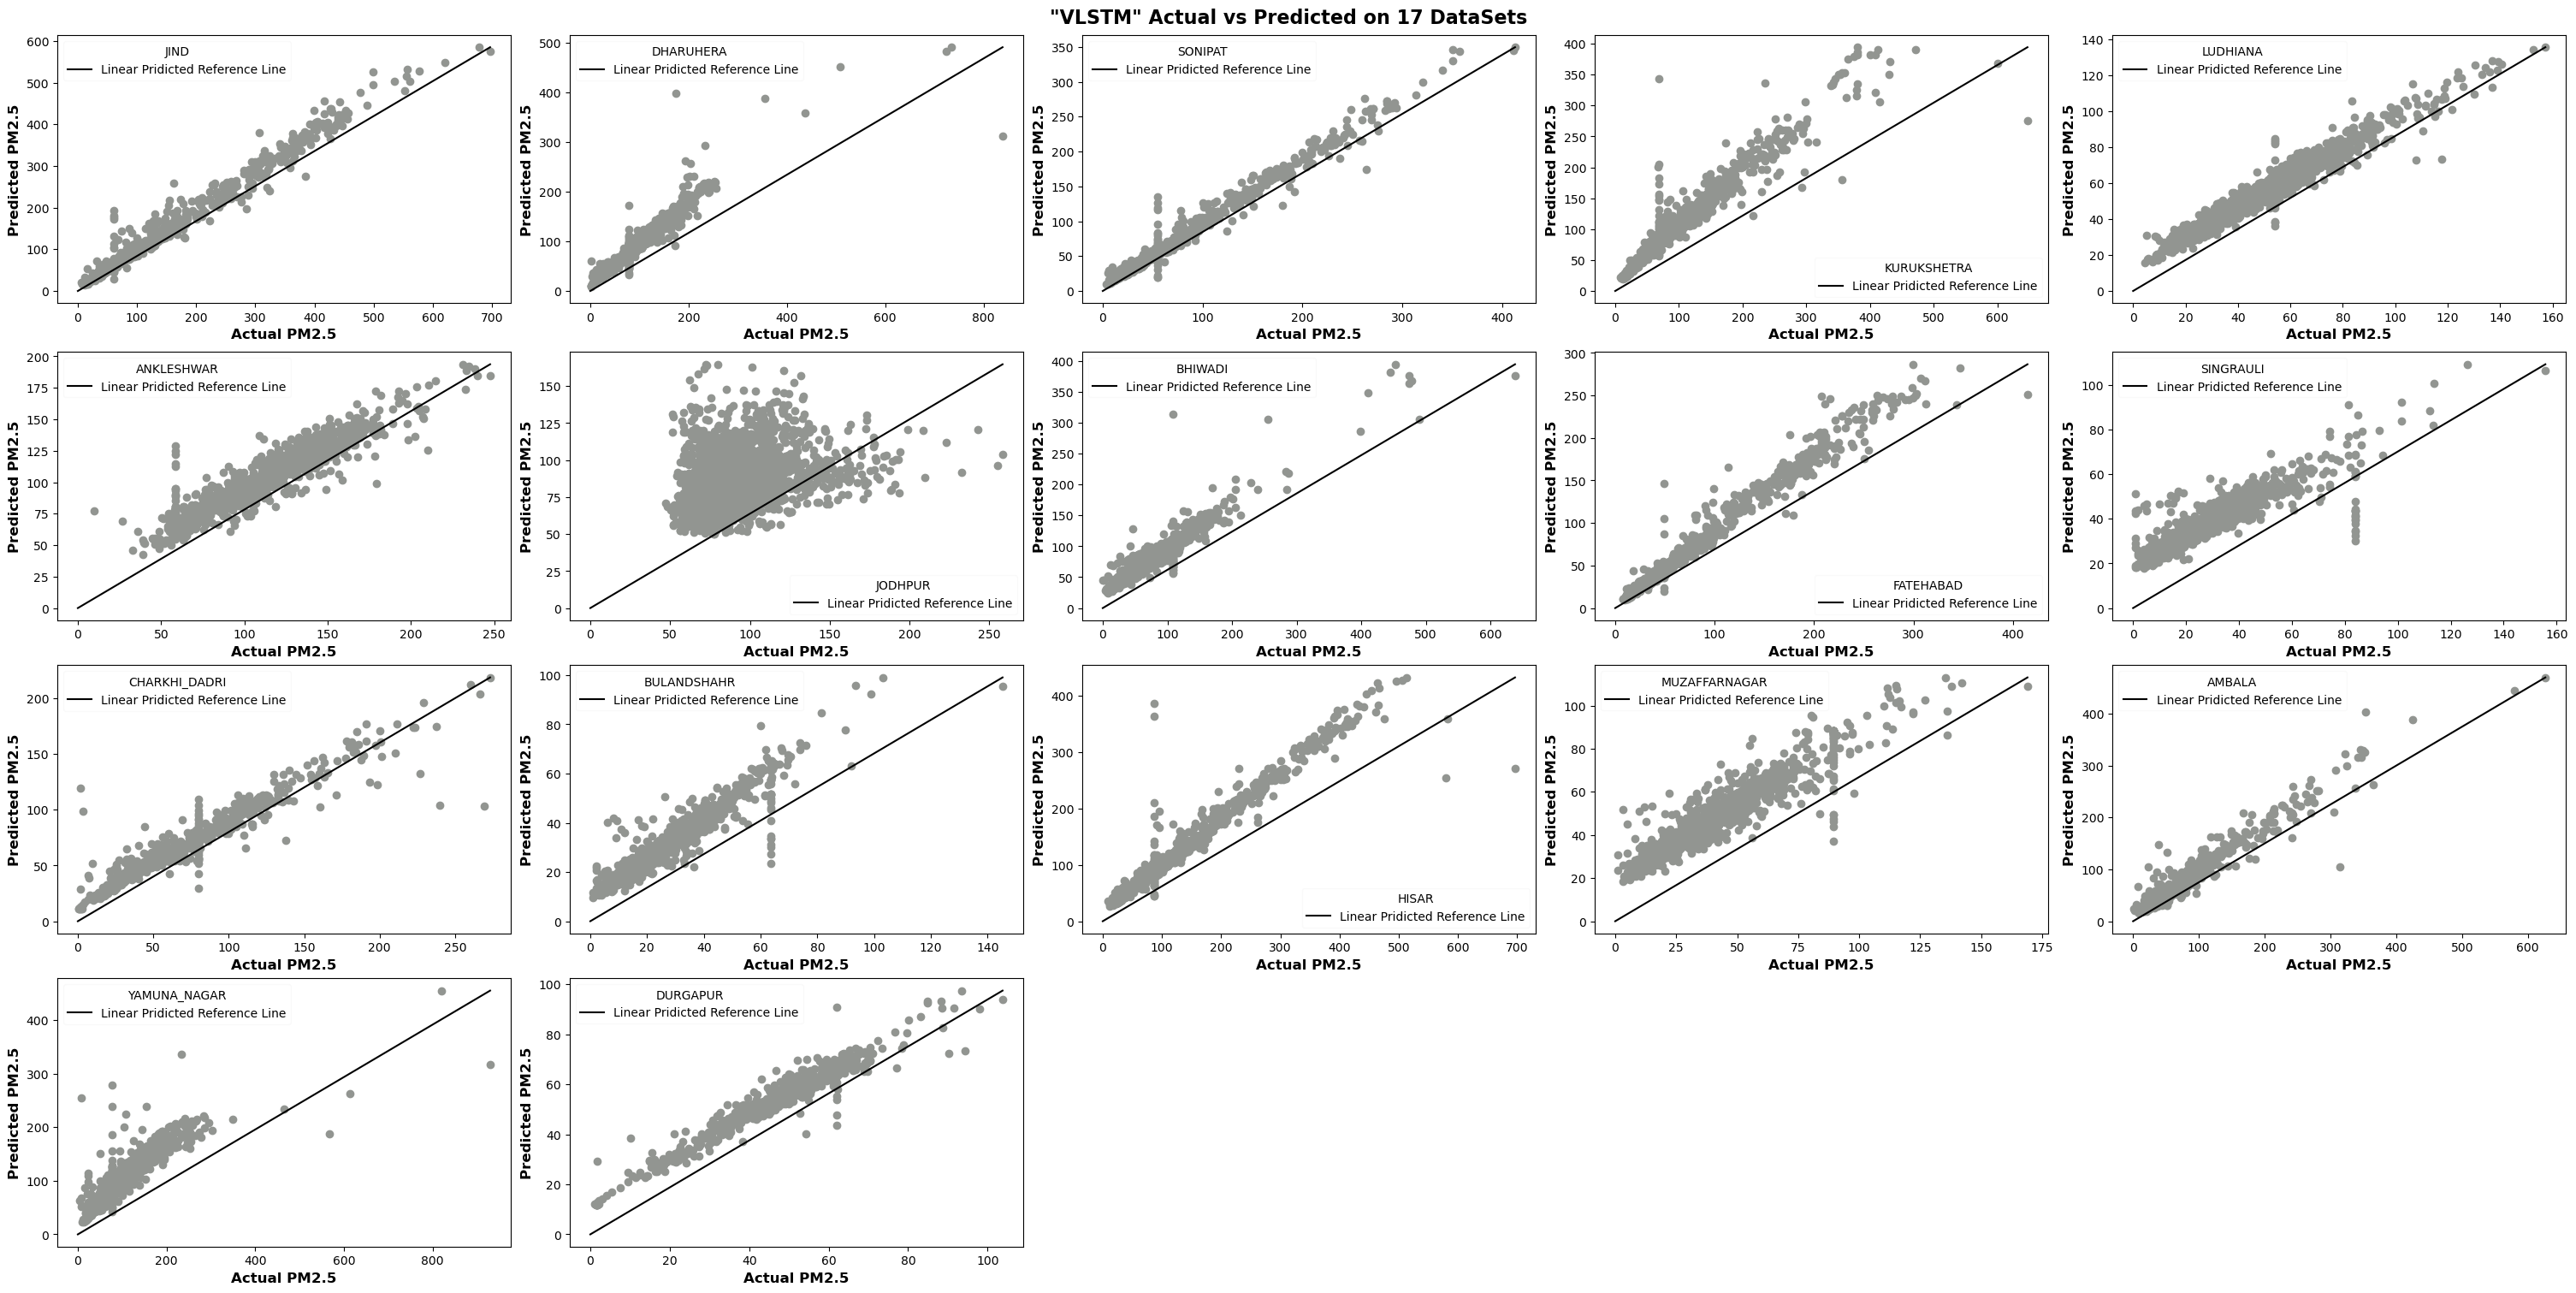
\includegraphics[scale=.18]{VLSTM}\\
% 	\scriptsize{FIGURE 5.4: Scattered plot of V-LSTM on 17 Indian Cities Dataset.}
% \end{frame}

\begin{frame}{Results and Analysis \tiny{Continue...}}
	\centering
	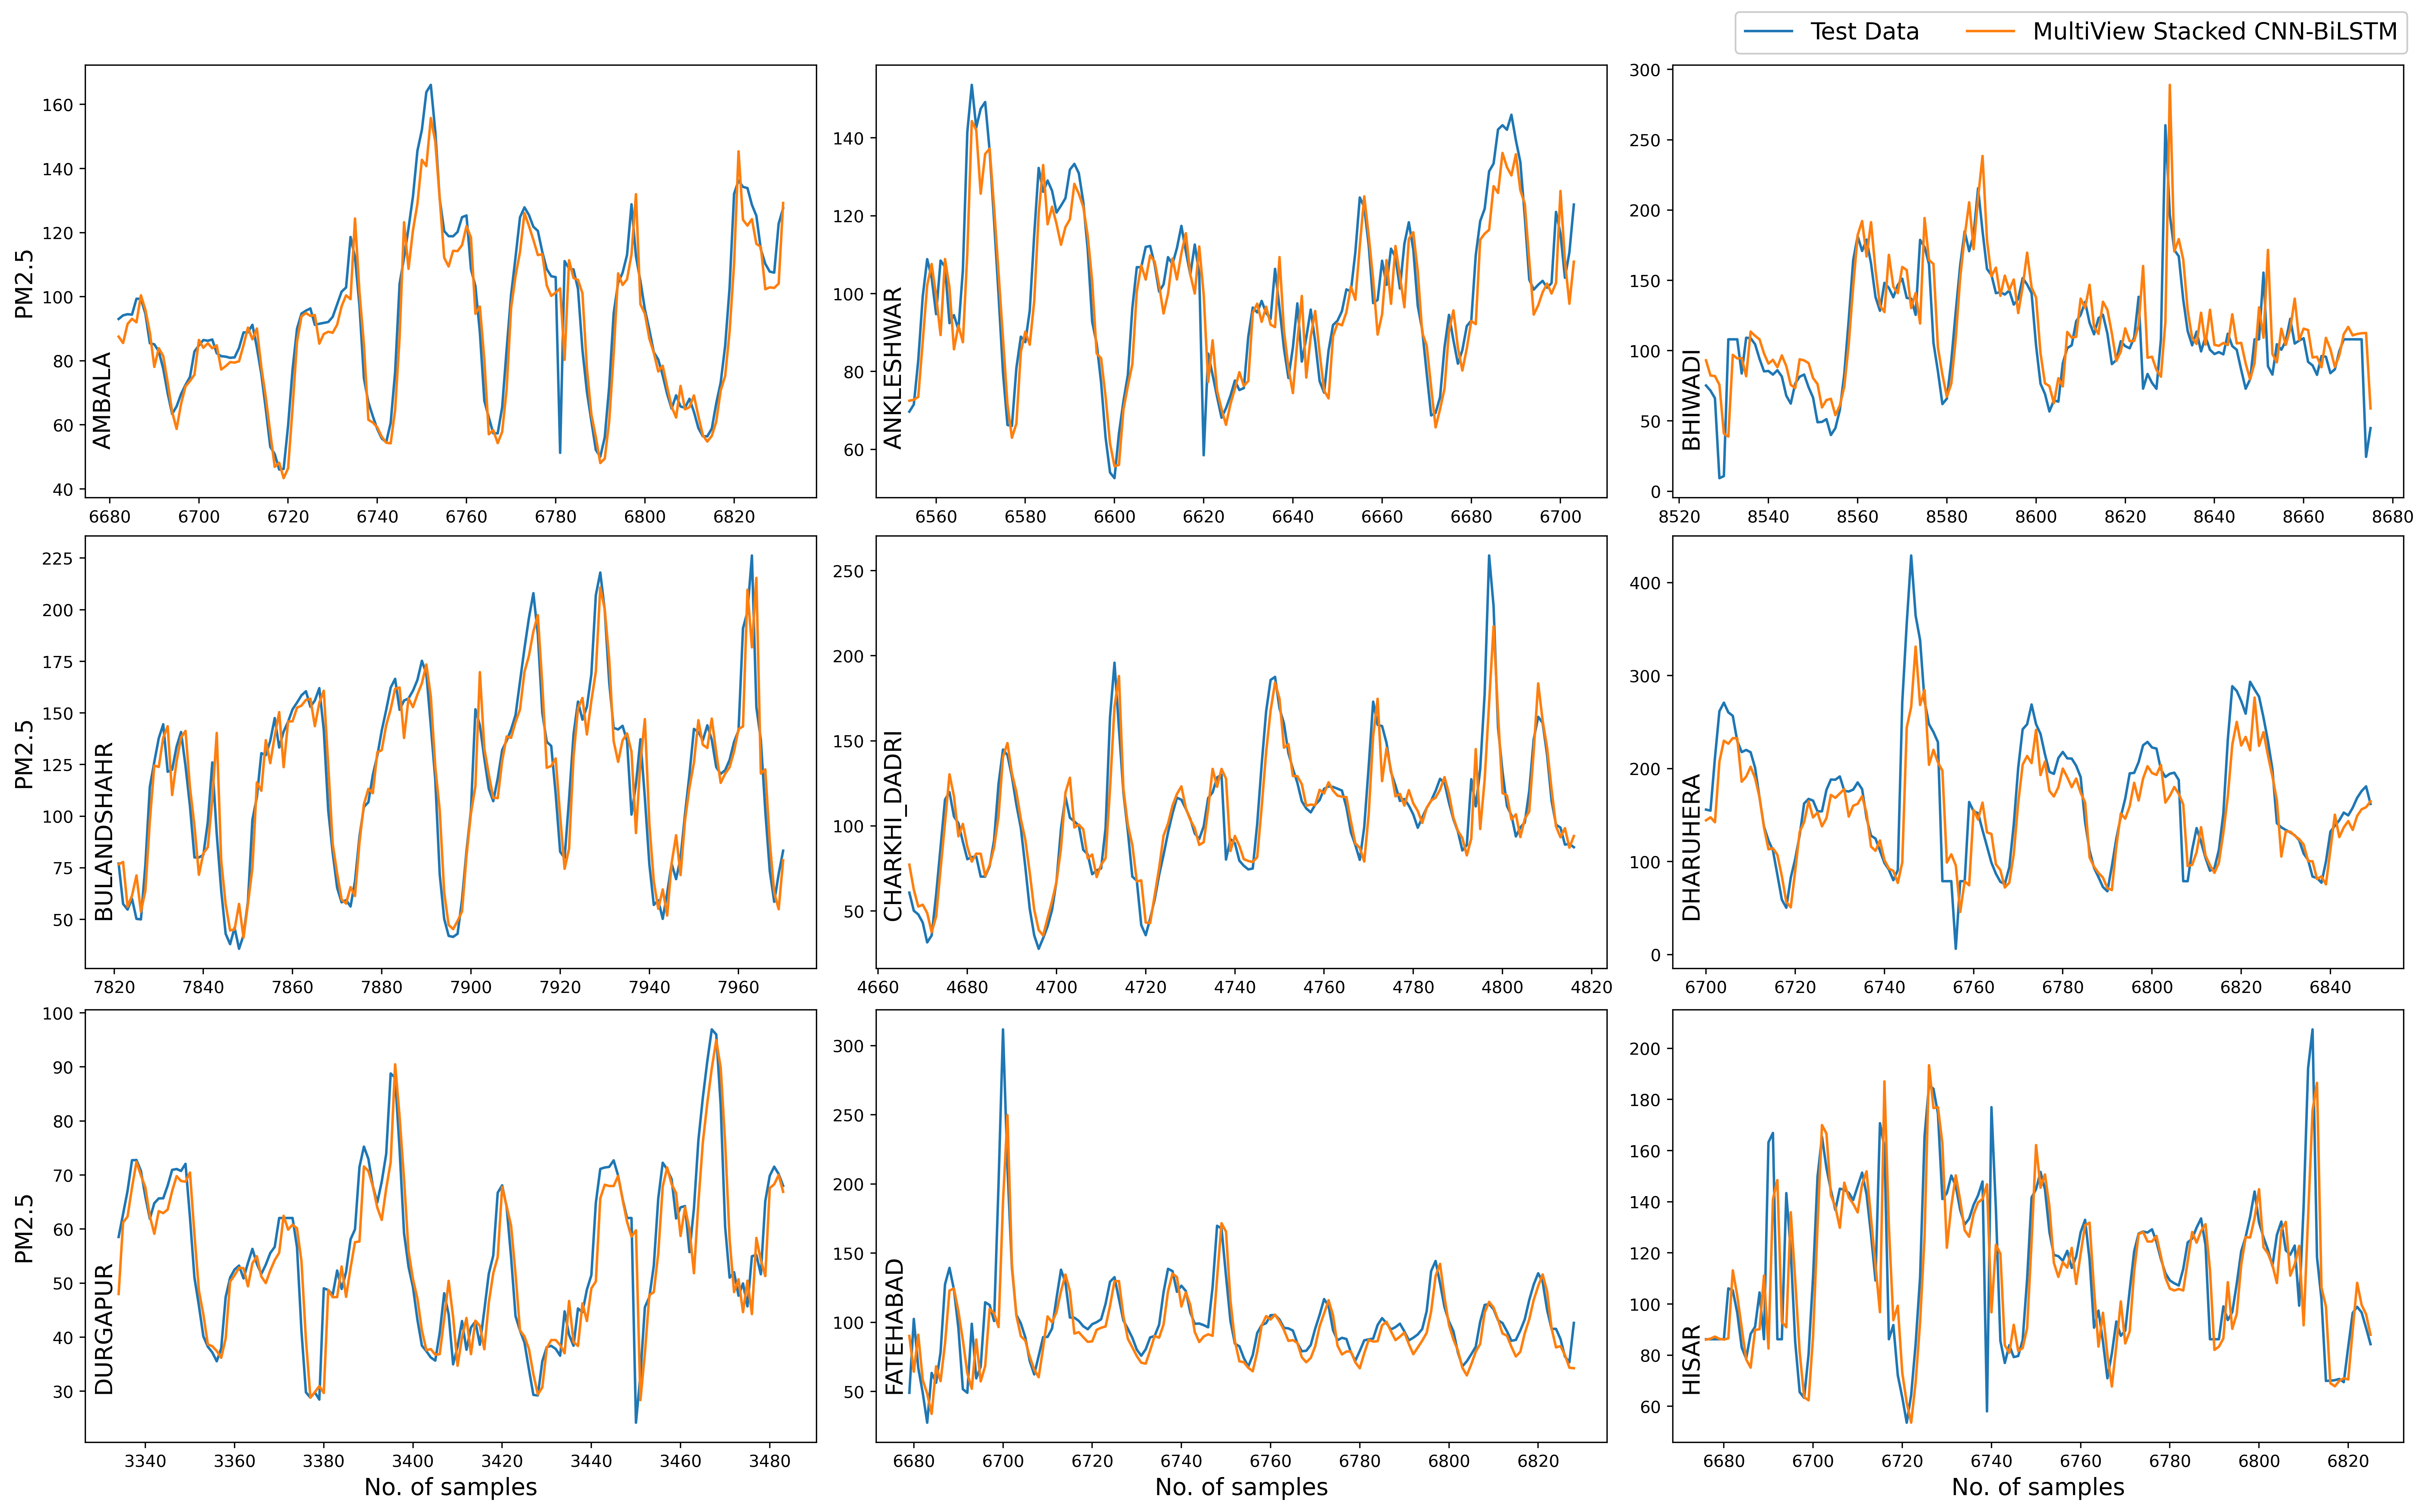
\includegraphics[scale=.218]{act vs pri}\\
	\scriptsize{FIGURE 5.1: $PM_{2.5}$ predictions of proposed models MvS CNN-BiLSTM}
\end{frame}


% \begin{frame}{Results and Analysis \tiny{Continue...}}
% 	\centering
% 	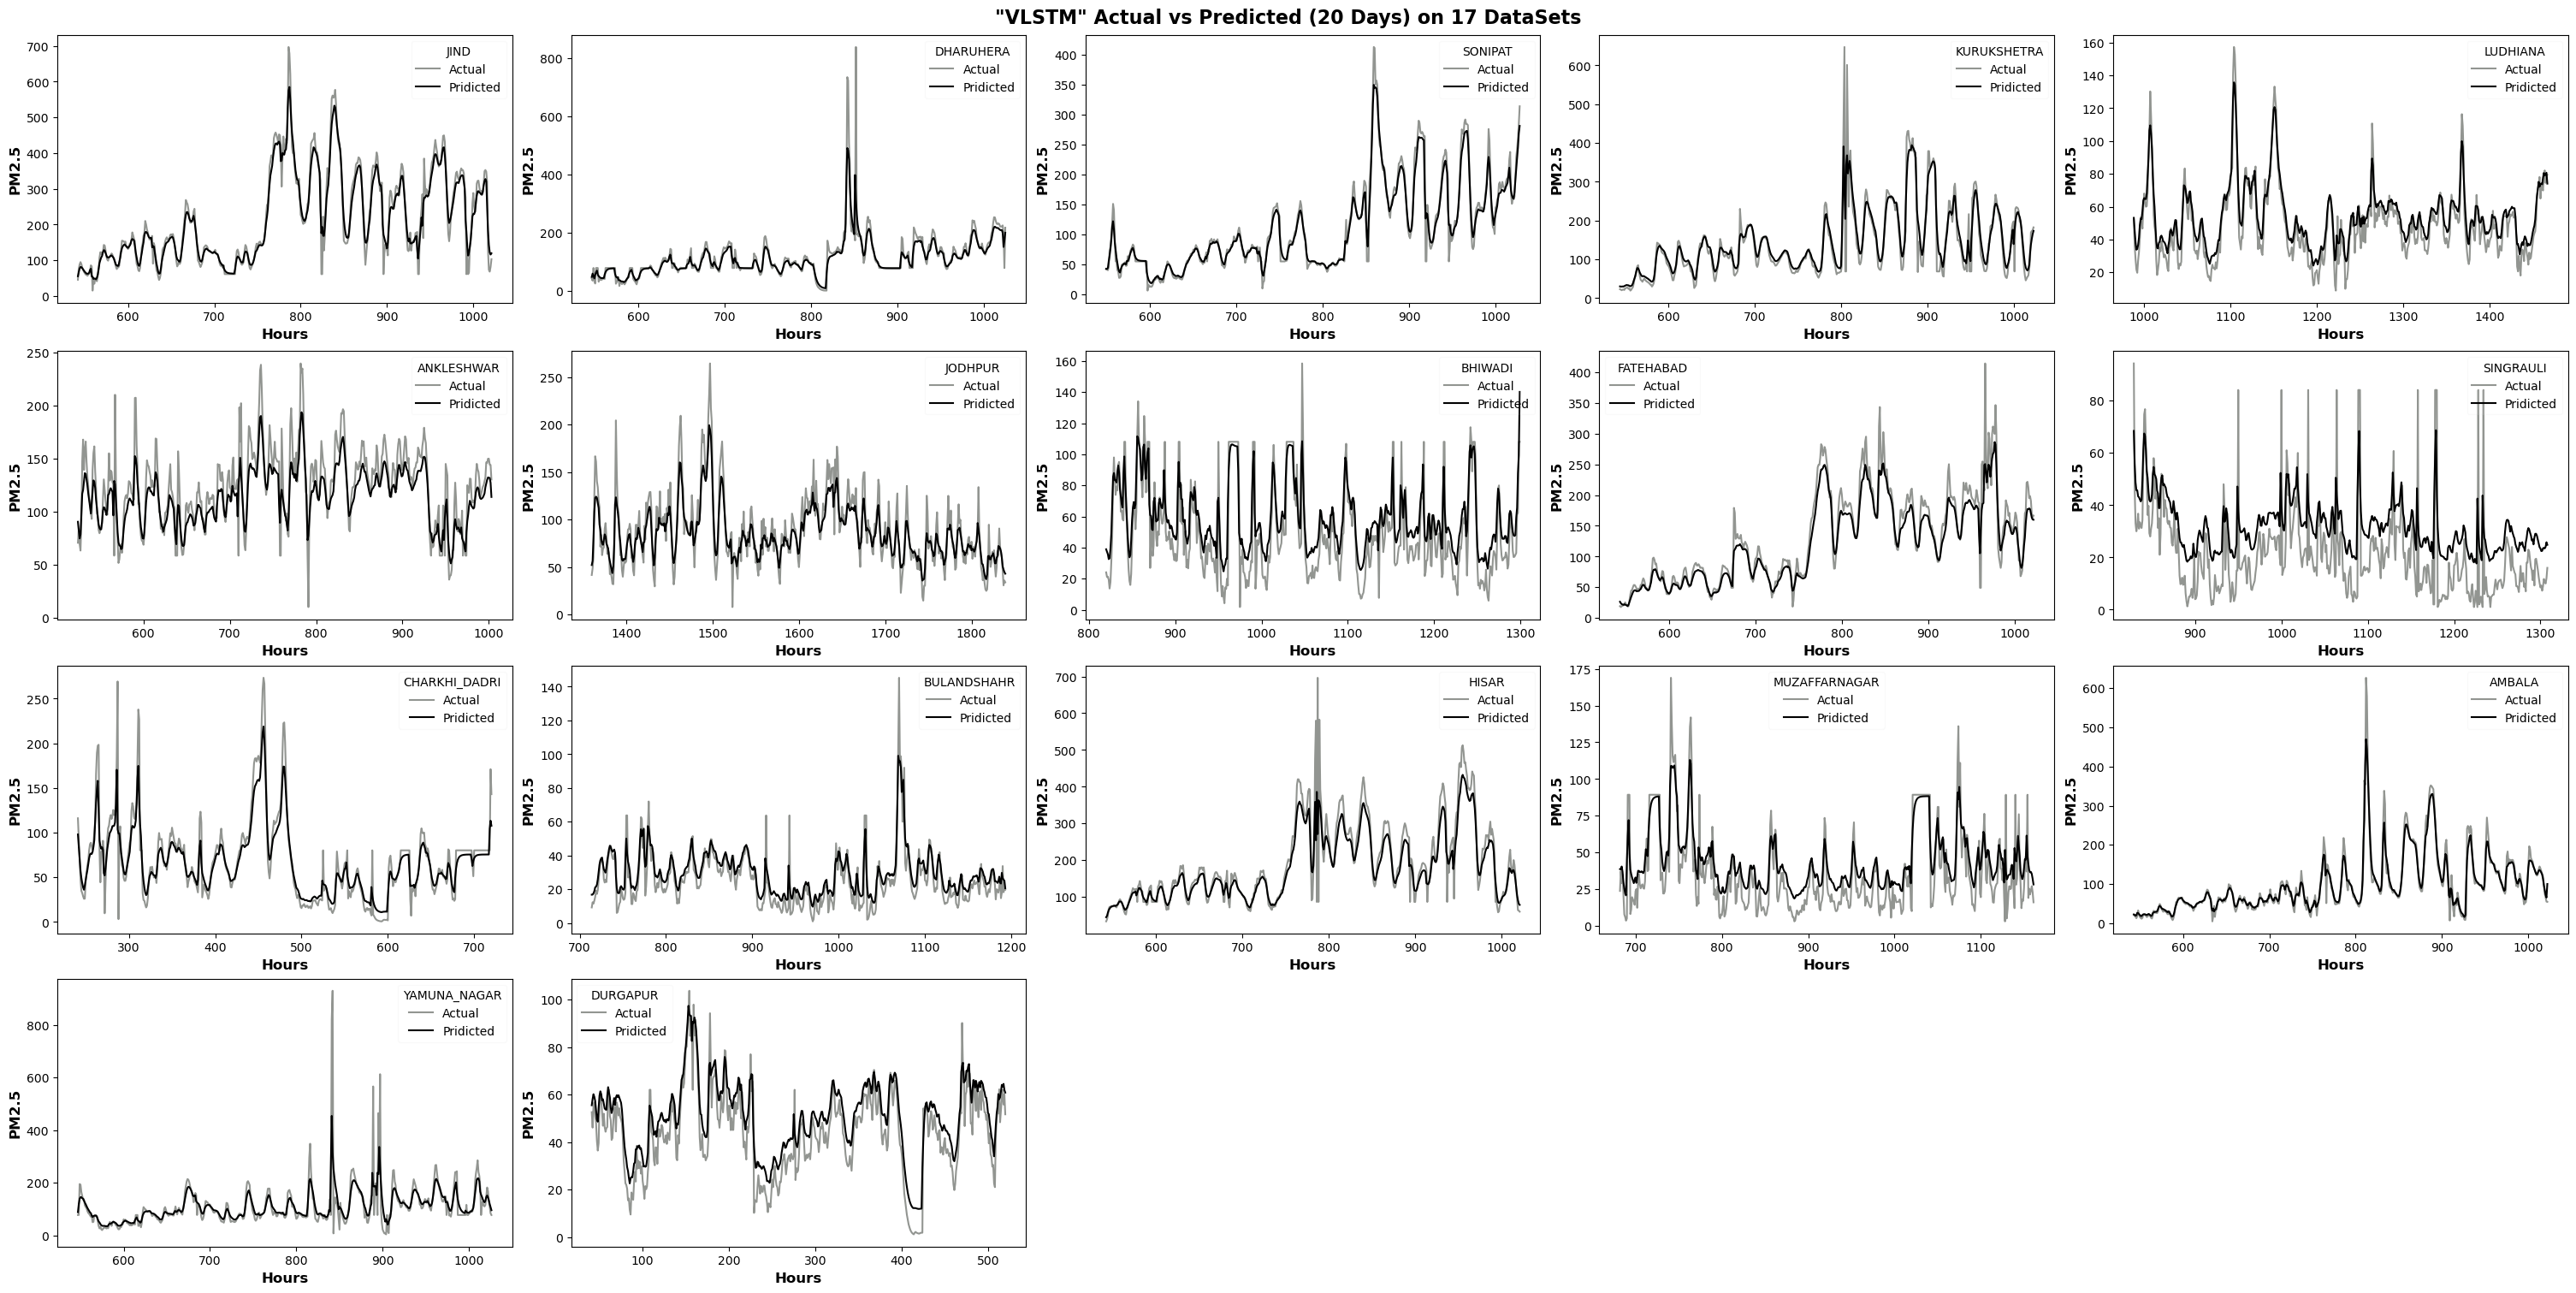
\includegraphics[scale=.18]{VLSTM(11)}\\
% 	\scriptsize{FIGURE 5.6: Actual vs Predicted of V-LSTM on 17 Indian Cities Dataset.}
% \end{frame}

\begin{frame}{Results and Analysis \tiny{Continue...}}
	\centering
	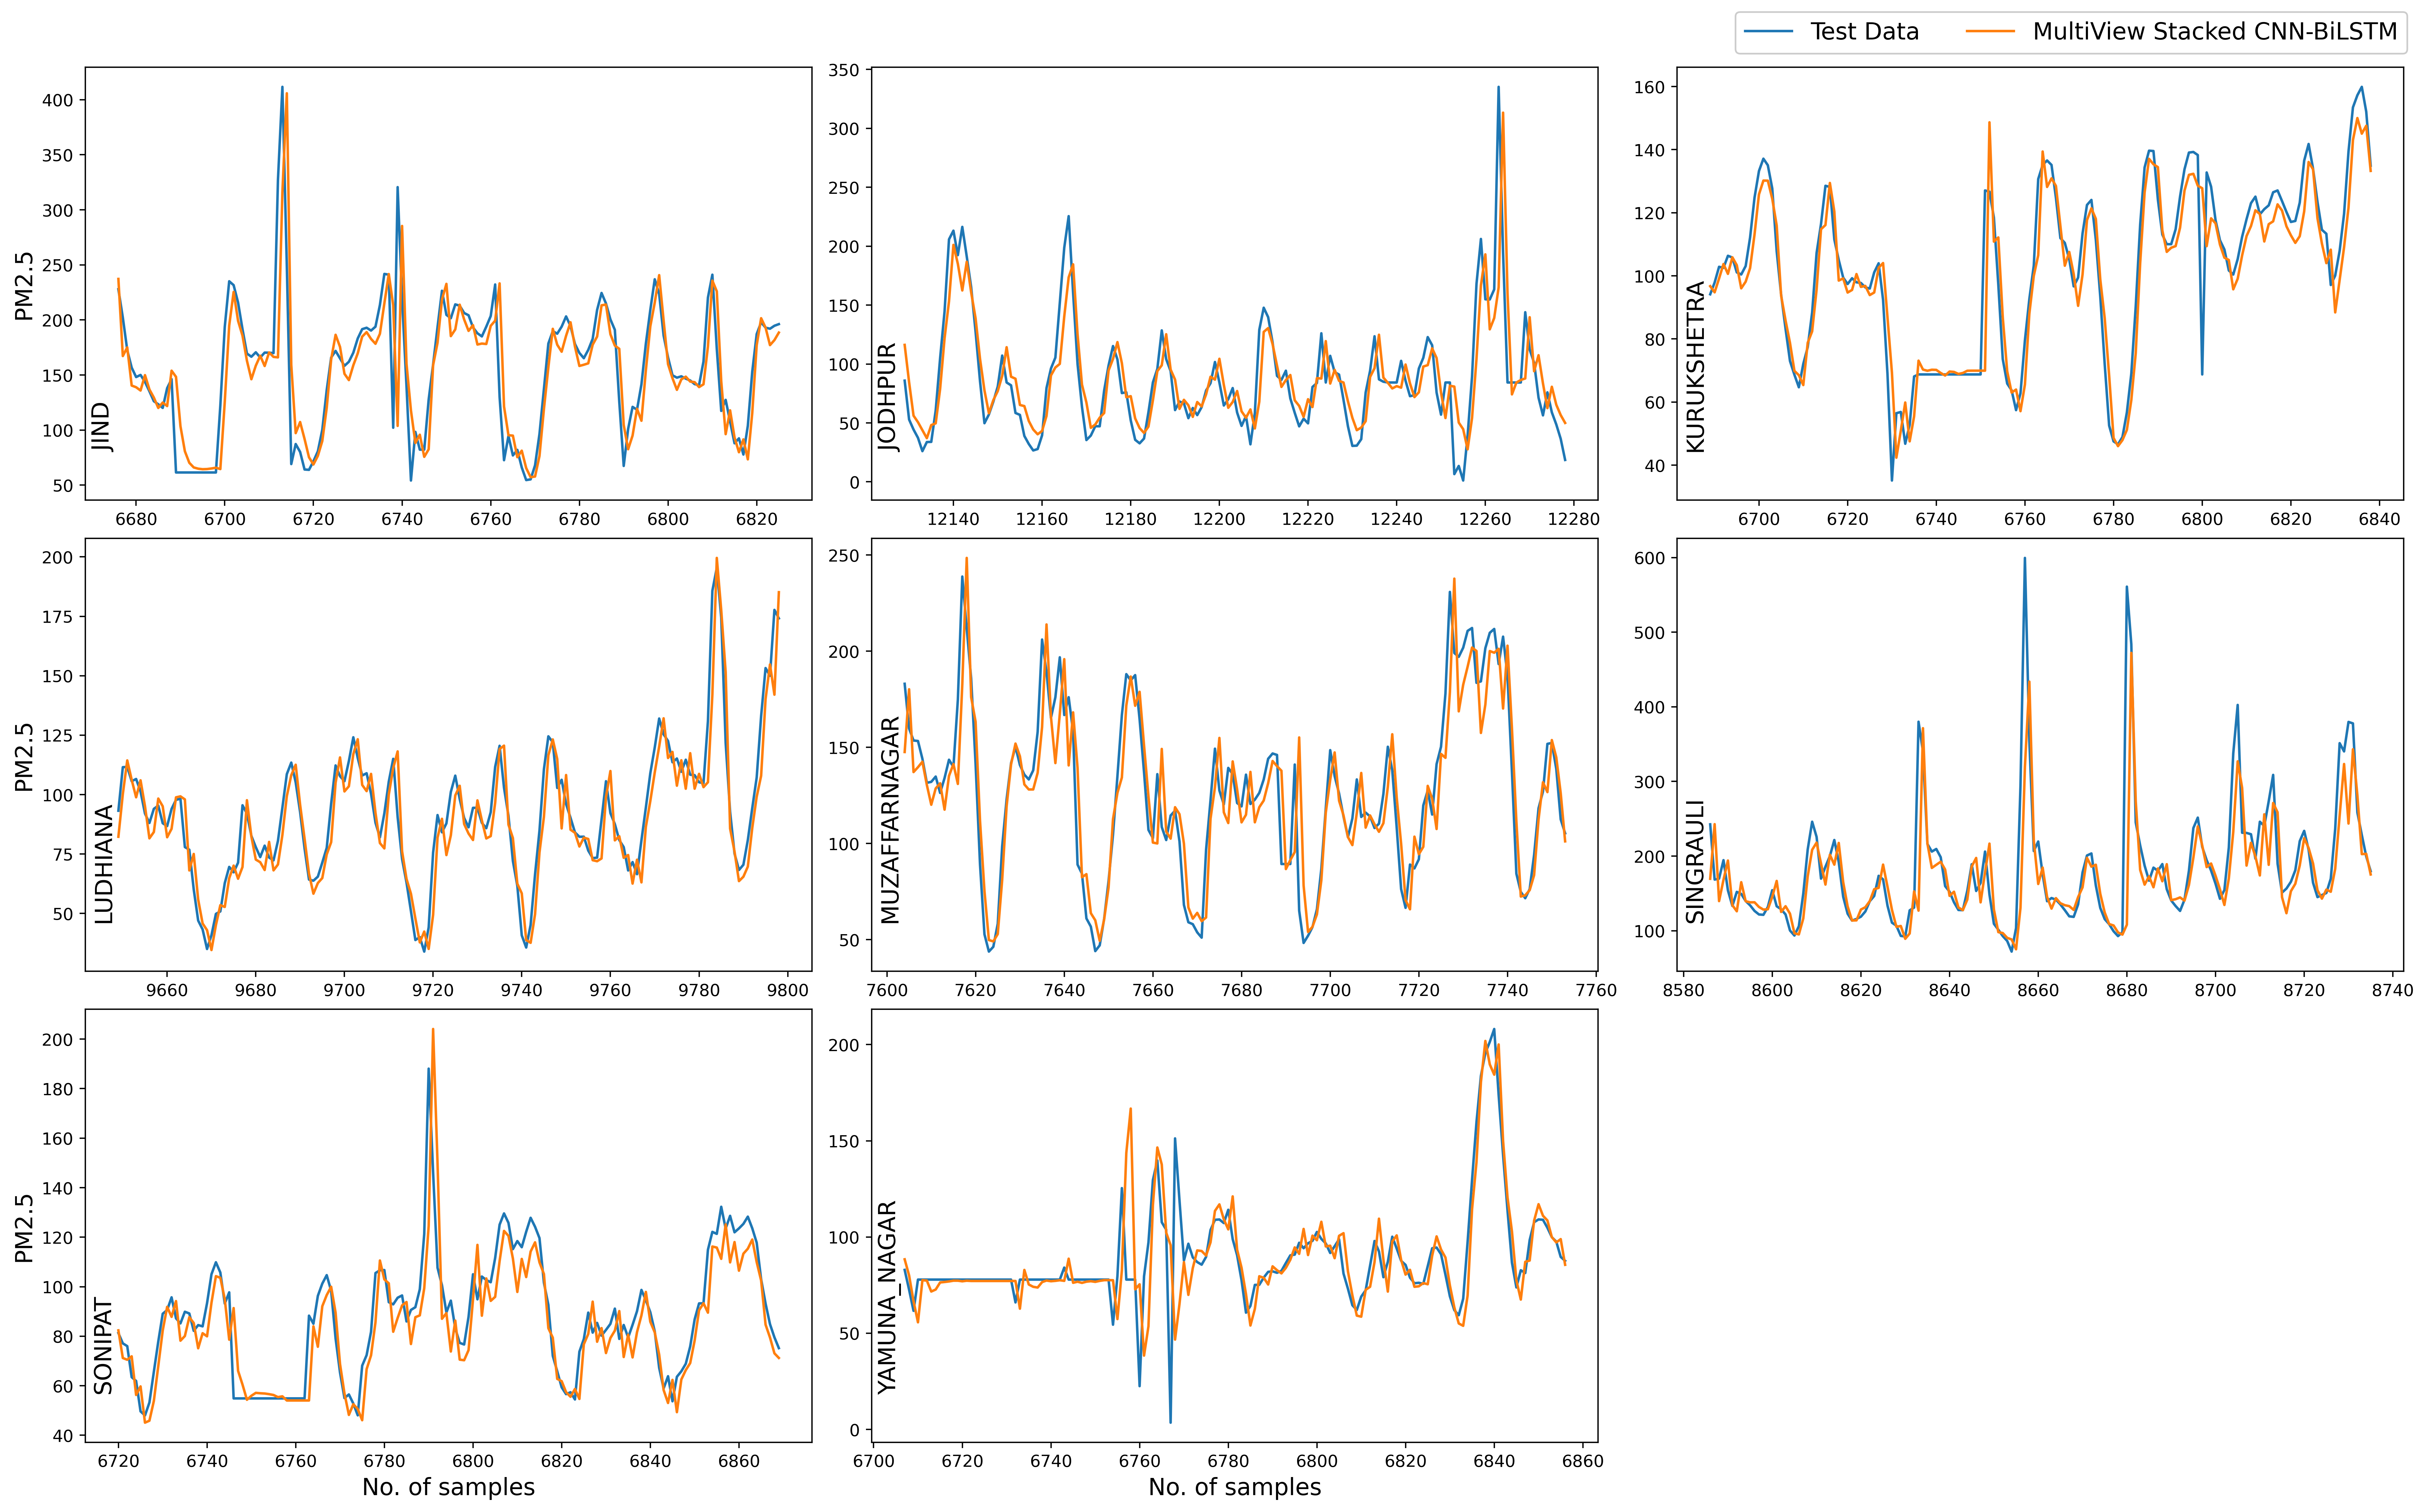
\includegraphics[scale=.218]{act vs pri1}\\
	\scriptsize{FIGURE 5.2: Continuation of $PM_{2.5}$ predictions of proposed models MvS CNN-BiLSTM}
\end{frame}


\begin{frame}{Results and Analysis \tiny{Continue...}}
	\centering
	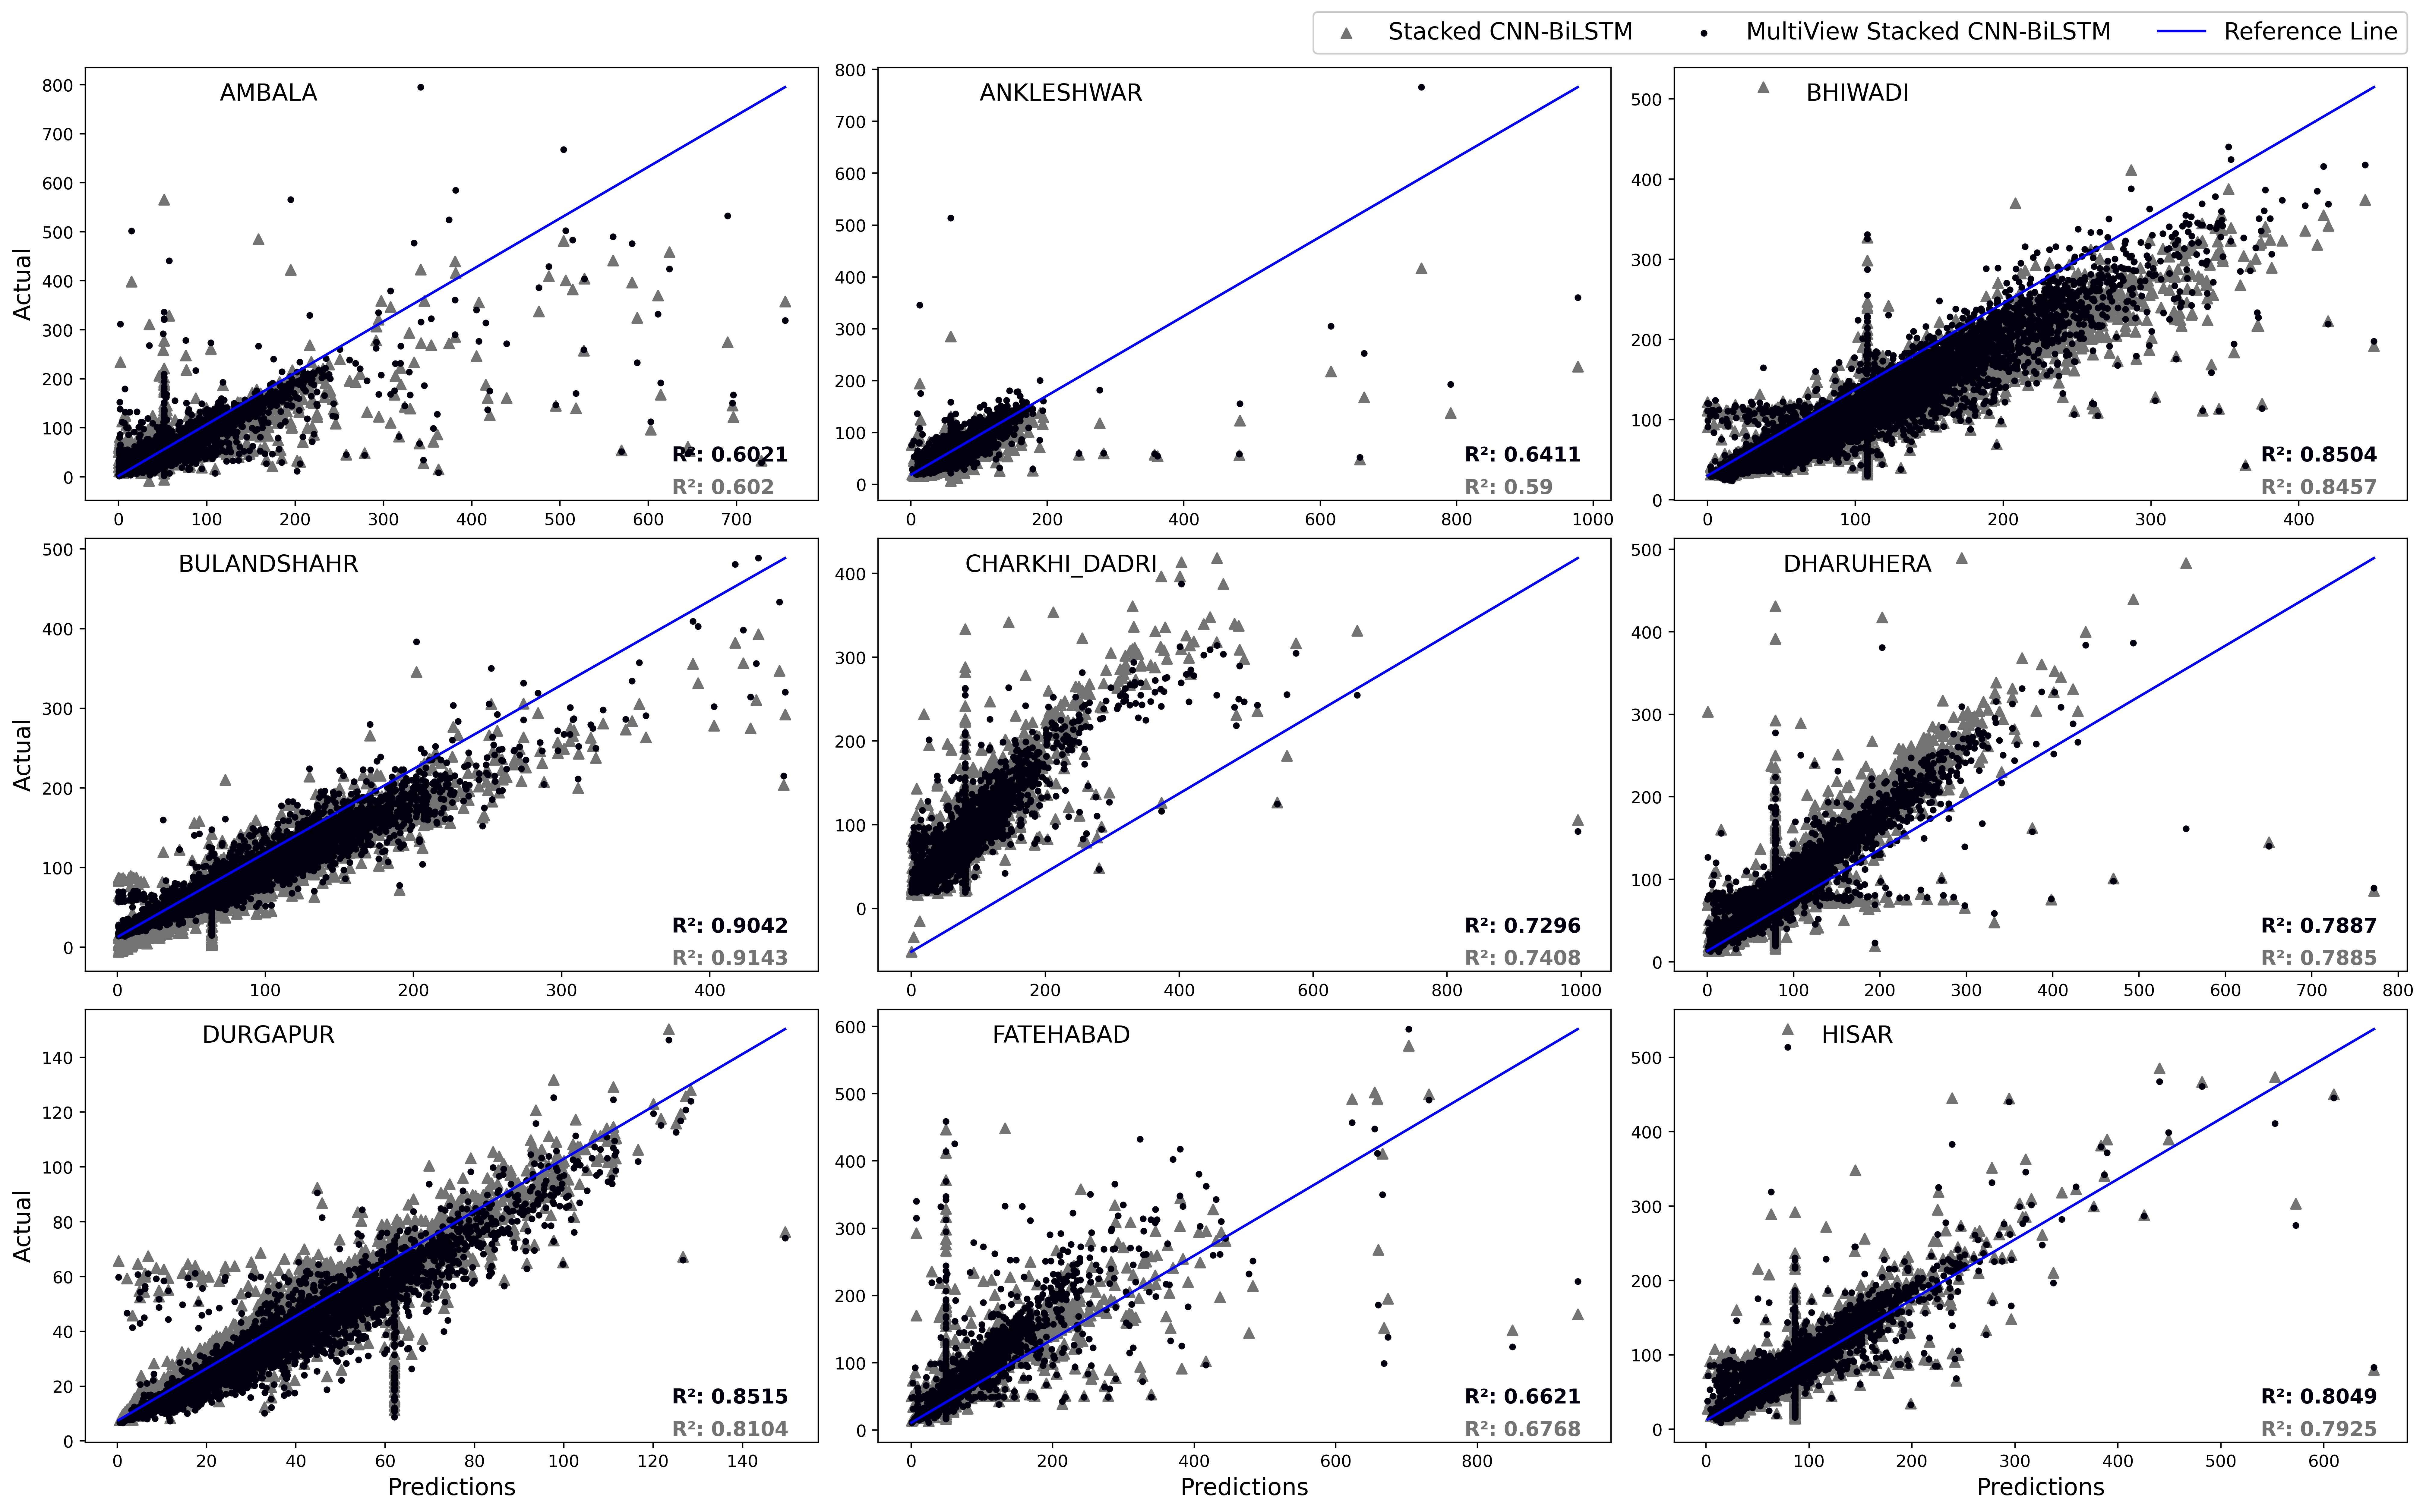
\includegraphics[scale=.218]{Scatter_plot}\\
	\scriptsize{FIGURE 5.3: Correlation of Actual values and Predictions of proposed models $($Stacked CNN-BiLSTM and MvS CNN-BiLSTM $)$ using Scatter plot.}
\end{frame}
\begin{frame}{Results and Analysis \tiny{Continue...}}
	\centering
	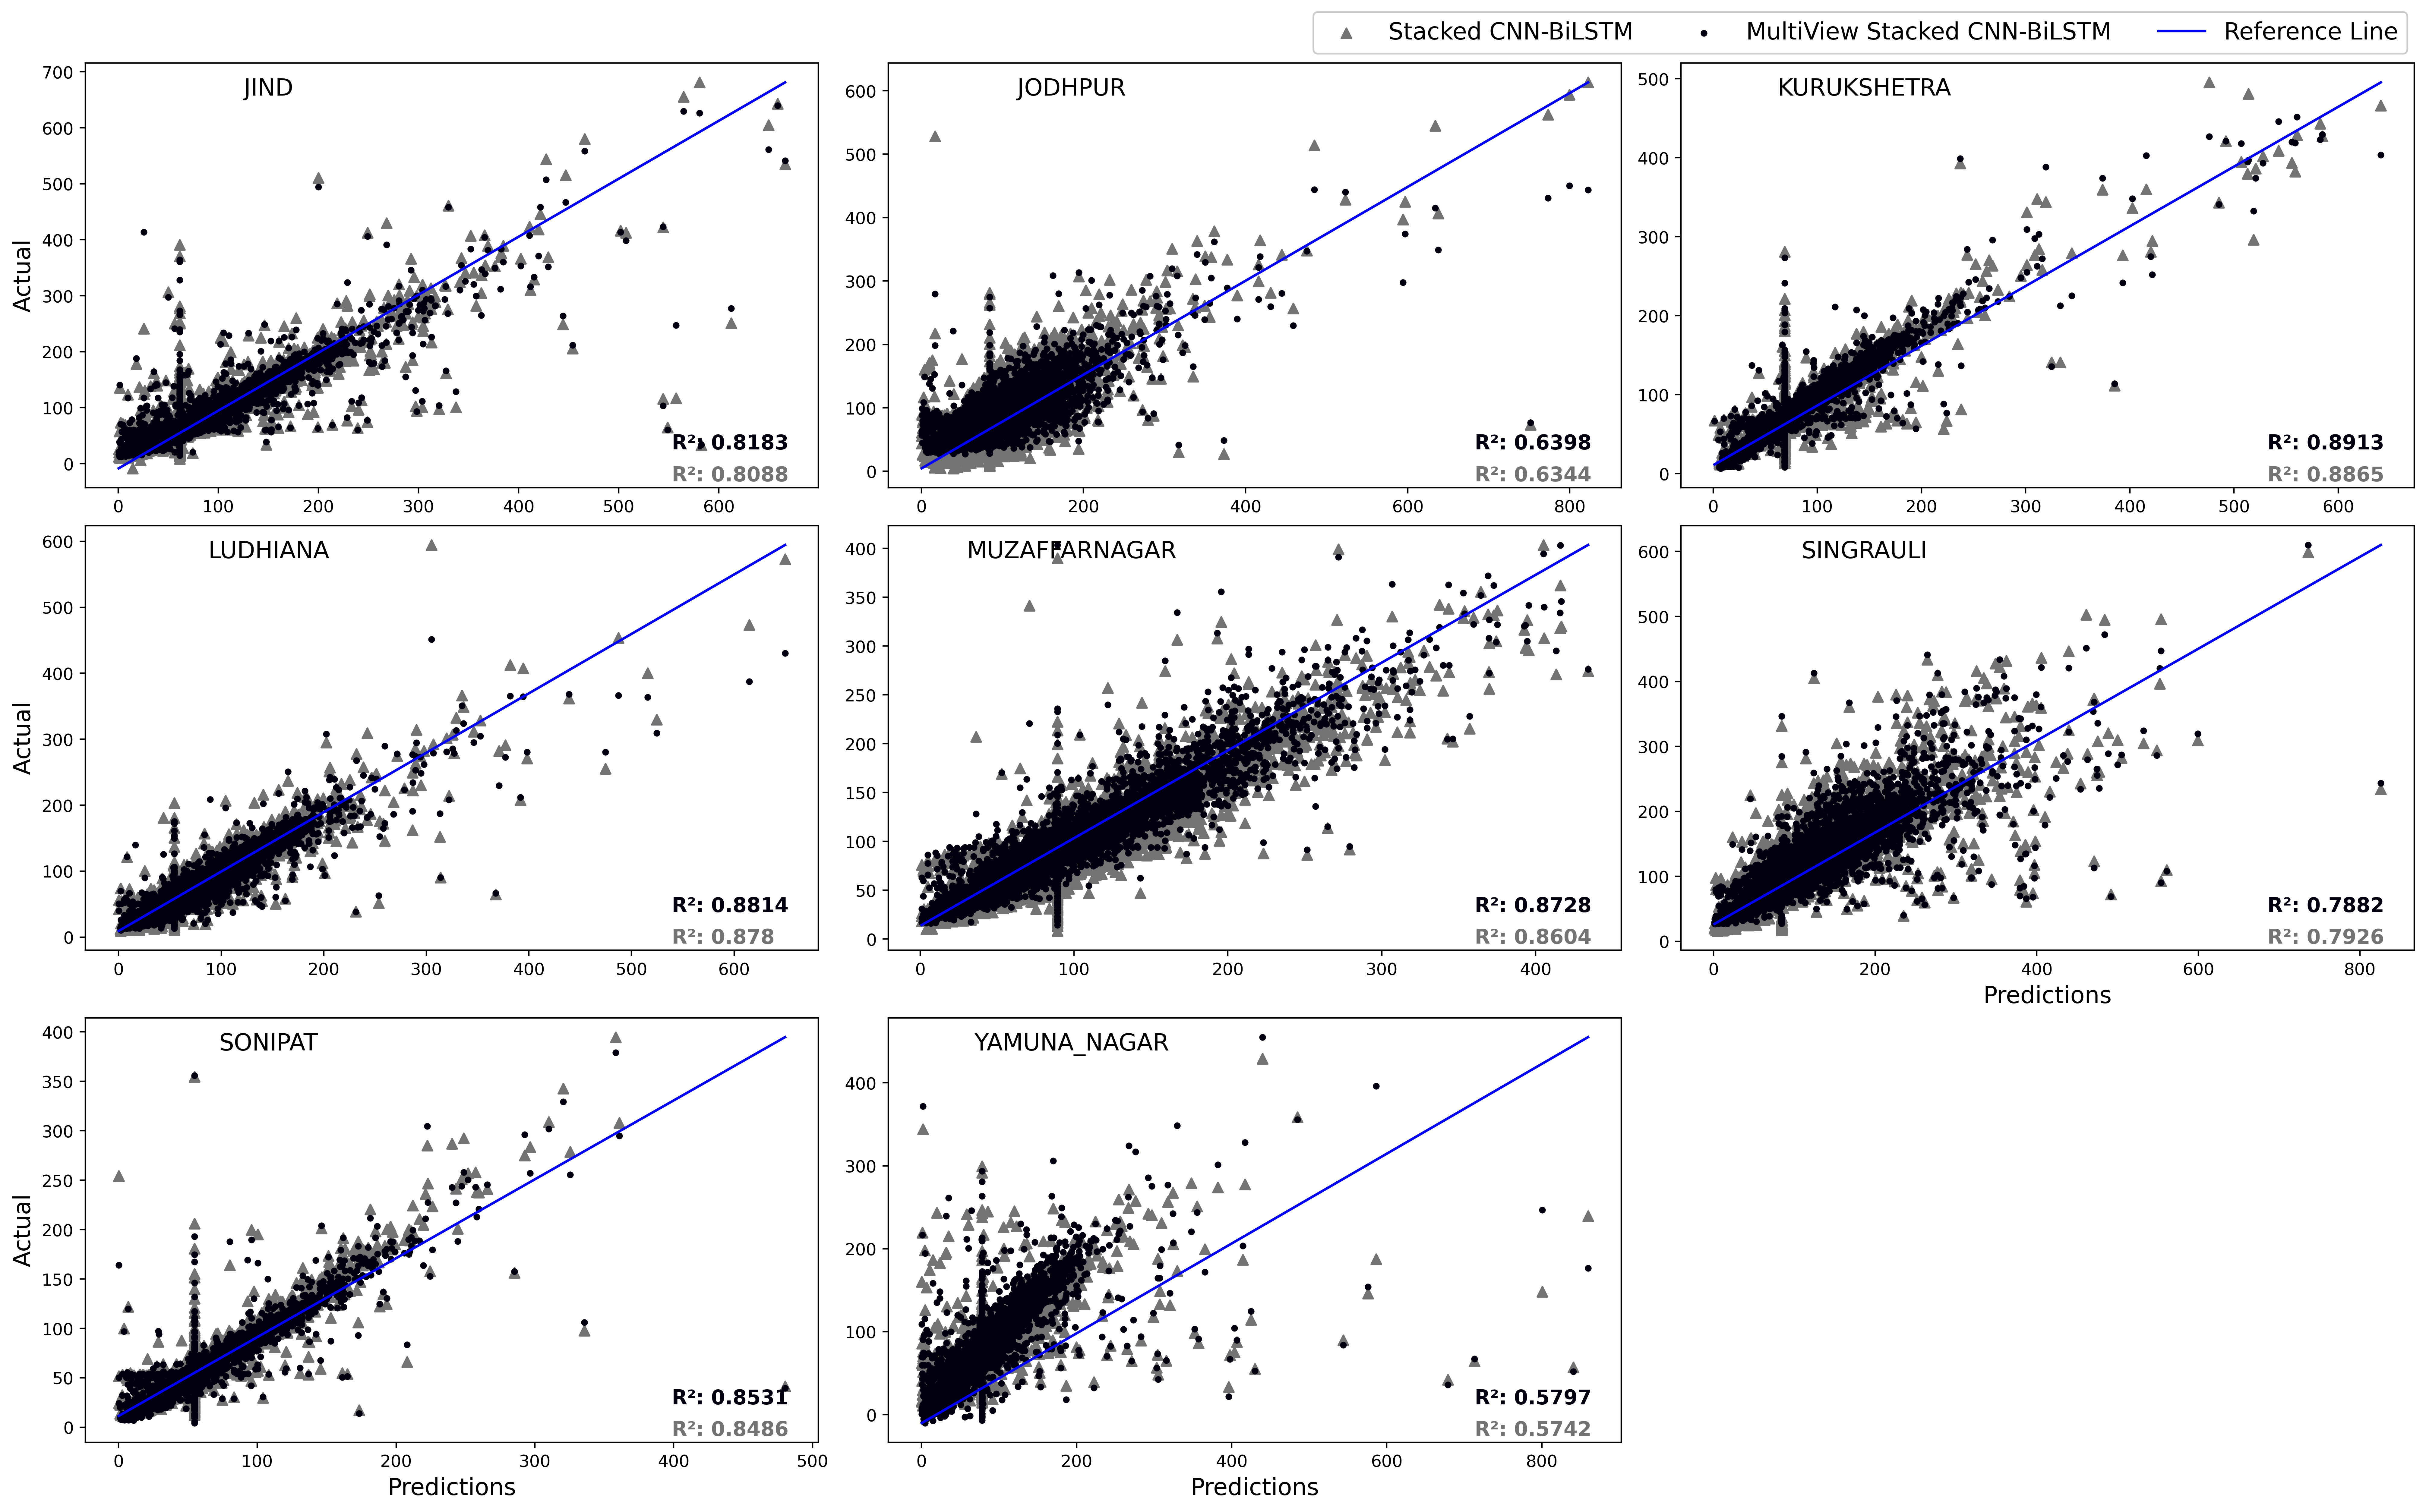
\includegraphics[scale=.218]{Scatter_plot1}\\
	\scriptsize{FIGURE 5.4: Continuation of correlation of Actual values and Predictions of proposed models $($Stacked CNN-BiLSTM and MvS CNN-BiLSTM $)$ using Scatter plot.}
\end{frame}

\begin{frame}{Results and Analysis \tiny{Continue...}}
\begin{table}
	\centering
	\scriptsize {TABLE 5.5: Overall average of RMSE and MAPE ranking of traditional models and proposed model (MvS CNN-BiLSTM).}
    \begin{tabular}[c]{ |p{0.19\linewidth} |p{0.16\linewidth}| p{0.16\linewidth} |p{0.16\linewidth}|  }
    \hline Algorithm&RMSE\_Ranking&MAPE\_Ranking&Average\_Ranking \\ \hline
    BiLSTM&3.7059&3.4706&3.58825\\
    CNN&4.8235&4.1765&4.5\\
    GRU&3.1765&3.7647&3.4706\\
    LSTM&3.8235&3.8824&3.85295\\
    RNN&3.7059&4.7059&4.2059\\
    \textbf{MvS CNN-BiLSTM}&\textbf{1.7647}&\textbf{1}&\textbf{1.38235} \\\hline
    \end{tabular}
    \end{table}
\end{frame}

\begin{frame}{Results and Analysis \tiny{Continue...}}
	\centering
	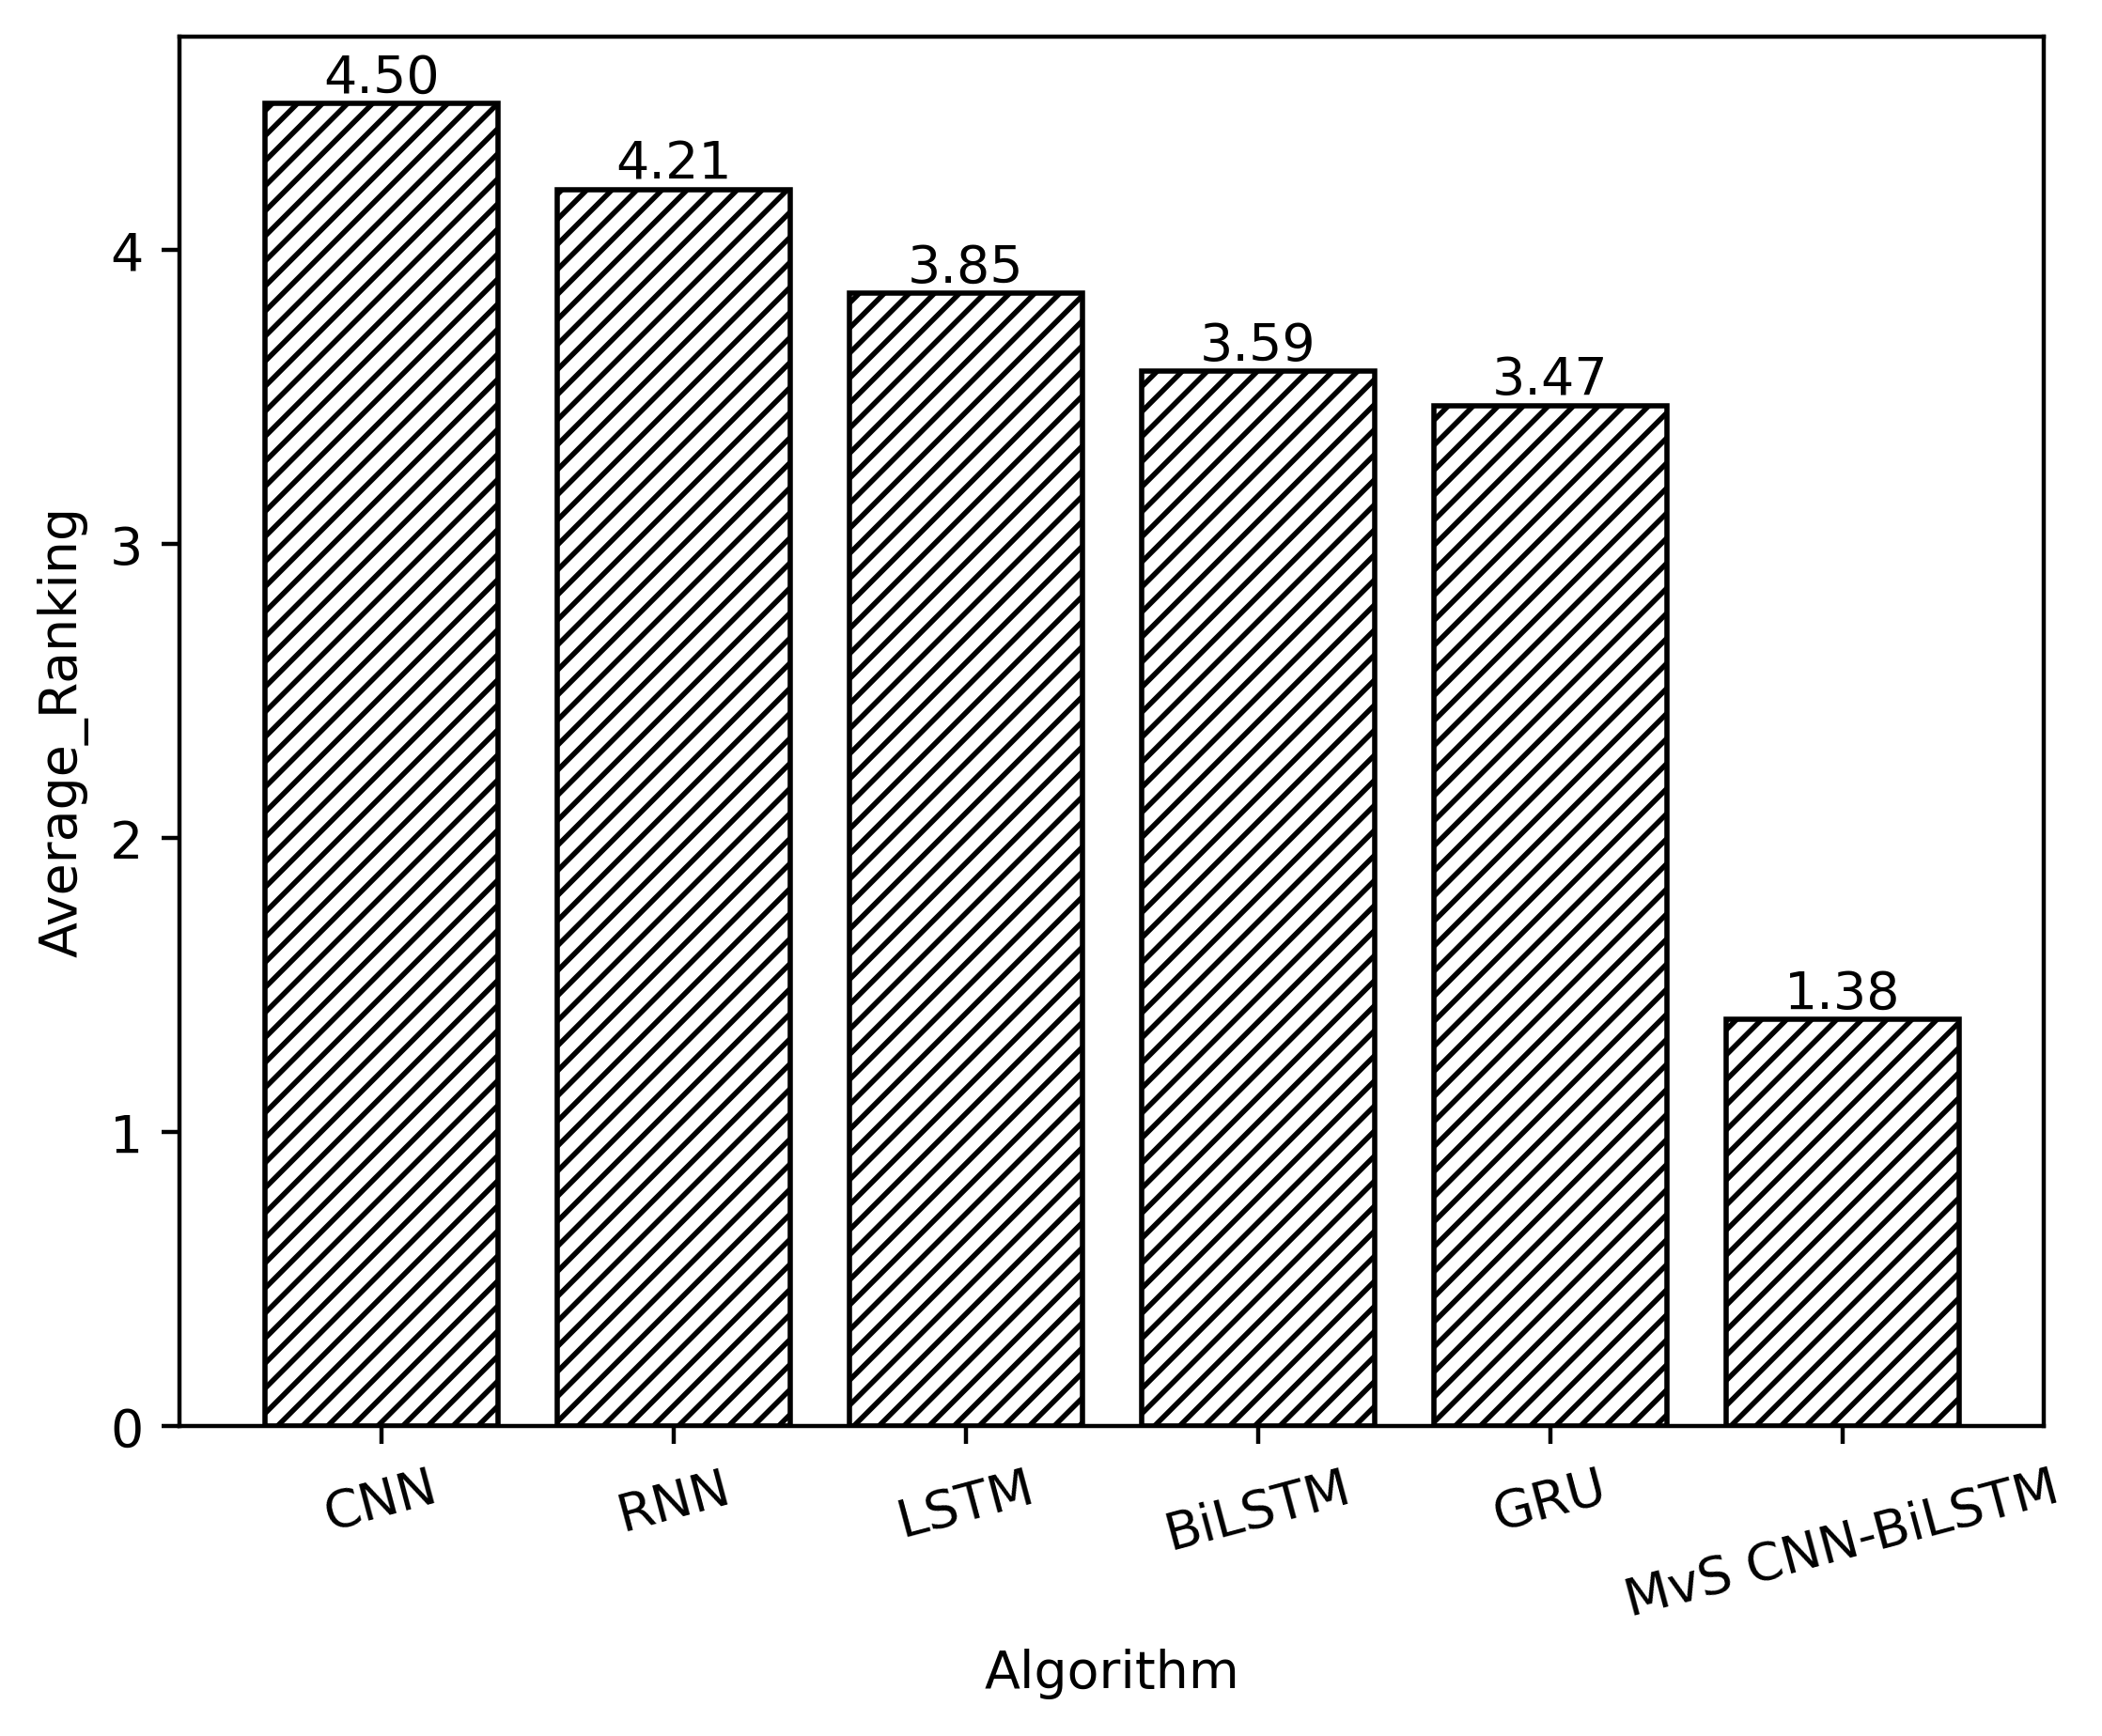
\includegraphics[scale=.5]{avg_Rank_plot}\\
	\scriptsize{FIGURE 5.5: Overall average Friedman ranking of traditional models and proposed MvS CNN-BiLSTM model.}
\end{frame}
%--------------------------------------------------------------------------
\section{Conclusions}
%--------------------------------------------------------------------------

\begin{frame}{Conclusions}
	\begin{block}{}
		\footnotesize {In this study, a hybrid MvS CNN-BiLSTM model has been proposed. The model utilises stacked 1D CNN \& BiLSTM as new architecture to view the univariate data $PM_{2.5}$ pollutant. Additionally, a novel multi-view approach has been proposed for univariate time series, which exploits the seasonal characteristics of the data to construct the views corresponding to the lowest lag. The seventeen datasets ($PM_{2.5}$) of highly polluted cities of India have been used to deploy the proposed MvS CNN-BiLSTM and stand-alone DL models. The evaluation of the models has been performed using RMSE and MAPE. The results have shown that the proposed model has improved the performed than corresponding stand-alone DL models over RMSE:  7.11\% (CNN), 5.08\% (RNN), 3.80\% (GRU), 5.57\% (LSTM) and 4.05\% (BiLSTM) and MAPE: 27.16\% (CNN), 28.52\% (RNN), 26.22\% (GRU), 27.22\% (LSTM), 23.11\% (BiLSTM). Moreover, the enhanced performance of the proposed model has also been validated using non-parametric statistical methods, i.e., Friedman ranking and Holm's procedure. The statistical analysis of results concludes that the proposed model performance is better and distinct from stand-alone DL models.}
	\end{block}
\end{frame}

\begin{frame}{Future Work}
	\begin{block}{}
		The proposed model has utilised two-stacked CNN-BiLSTM for this research, where multiple combinations of stand-alone DL models may be investigated along with the stacking of the hybrid for better performance. In a multi-view approach, apart from seasonal characteristics, trends and the remainder may be utilised to generate the views of the dataset, yielding enhanced performance. Moreover feature set partitioning method of multi-view learning may be utilised for multivariate time series data (single source or multi-source data).
	\end{block}
\end{frame}


%..........................................................................
%\section{}
%..........................................................................

%--------------------------------------------------------------------------
%\section{References}
%--------------------------------------------------------------------------

%\begin{frame}[t, allowframebreaks]{References}
%	
%\scriptsize
%\begin{thebibliography}{9}
%	\bibitem{allen13} Allen, Theresa M. and Pieter R. Cullis. Liposomal drug delivery systems: from concept to clinical applications, \emph{Adv. drug del. Rev.}, 65(2013)36--48.
%	
%	\bibitem{saffman} Saffman P. G. and Taylor G., The penetration of a fluid into a medium of Hele-Shaw c58ell containing a more viscous liquid, \emph{Proc. Soc. London, Ser A}, 245(1958)312-329.
%	
%	\bibitem{sopan13} Sunthar, P. and Phappal, S. M.,  Influence of micro-mixing on the size of liposomes self-assembled from miscible liquid phases. \emph{Chem. phys. lipids}, 172-173(2013)20-30.
%	
%\end{thebibliography}
\begin{frame}[t, allowframebreaks]{References}
\bibliographystyle{IEEEtran}
\bibliography{mybib}

\end{frame}


%--------------------------------------------------------------------------
%\section{Query}
%--------------------------------------------------------------------------

\begin{frame}[plain]{ }
	\centering
	\Huge {Thank You.}

\end{frame}
	
\end{document}
%===========================================================================================